\documentclass[twoside,12pt]{report}
\usepackage[T1]{fontenc}
\usepackage[utf8]{inputenc}
\usepackage[magyar]{babel}
\usepackage[margin=3cm]{geometry}
\usepackage[section]{placeins}
\usepackage{amsmath,amssymb,tikz,fancyhdr,commath,multirow,amsthm,gensymb,etoolbox,csquotes,float,outlines,mathtools,pgfplots,makecell,yhmath}
\setquotestyle[quotes]{german}
\usetikzlibrary{shapes,decorations.pathreplacing,arrows,fit}

\title{Tételek: Matematika}
\author{Horváth Dávid}
\graphicspath{{Figures/}}
\newcommand\getcurrentref[1]{%
	\ifnumequal{\value{#1}}{0}
	{Tartalomjegyzék}
	{\the\value{#1}. tétel}%
}
\newcommand\addvmargin[1]{
	\node[fit=(current bounding box),inner ysep=#1,inner xsep=0]{};
}
\makeatletter
\newcommand{\ray}{%
	\mathpalette {\overarrow@\rayfill@}}
\def\rayfill@{\arrowfill@{\mkern4mu\mapstochar\relbar}\relbar{\mkern 4.08mu}}%
\makeatother
\renewcommand{\vec}{\underline}
\fancyhead[LE,RO]{\getcurrentref{chapter}}
\fancyhead[RE,LO]{Horváth Dávid}
\newtheorem{theorem}{Tétel}[section]
\theoremstyle{definition}
\newtheorem{definition}[theorem]{Definíció}
\newtheorem{claim}{Állítás}[theorem]
\linespread{1.3}
\setlength{\parskip}{0em}
\begin{document}
\pagestyle{fancy}
\maketitle
\tableofcontents
\pagebreak
\chapter{Halmazok}
\section{Halmazok, halmazműveletek}
	A halmaz és a halmaz eleme alapfogalom, ezért nem definiáljuk, azonban úgy kell megadjuk, hogy mindenről egyértelműen eldönthető legyen, eleme vagy sem.
	
	A halmazokat nyomtatott nagybetűvel, a halmaz elemeit kisbetűvel jelöljük.
	
	\vspace{1 em}
	
	\noindent
	\textbf{Halmazok megadási módjai:}
	\begin{itemize}
		\item Elemek felsorolásával
			\subitem Pl.: A=\{0;2;4;6\}
		\item Elemeket egyértelműen meghatározó utasítással
			\subitem Pl.: B=\{páros számok\}
		\item Szimbólumokkal
			\subitem Pl.: A=\{$x|x^2>9$\}
		\item Venn-diagrammal
			\subitem 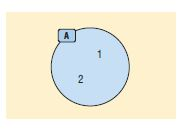
\includegraphics[]{Venn}
	\end{itemize}

	\begin{definition}
		Két halmaz egyenlő, ha ugyanazokat az elemeket tartalmazzák
	\end{definition}
	\begin{definition}
		Az elem nélküli halmazt üres halmaznak nevezzük.\\
		Jele:\{\}, vagy $\emptyset$
	\end{definition}
	\begin{definition}
		Az A halmaz részhalmaza a B halmaznak, ha A minden eleme a B halmaznak is eleme.\\
		Jele: $A\subseteq B$
	\end{definition}
	\begin{definition}
		Az A halmaz valódi részhalmaza a B halmaznak, ha A részhalmaza a B-nek, de nem
		egyenlő vele.\\
		Jele: $A\subset B$
	\end{definition}
	
	\noindent
	\textbf{Tulajdonságok:}
	\begin{itemize}
		\item $\emptyset\subseteq A$
		\item $A\subseteq A$
		\item $A\subseteq B \wedge B\subseteq A \implies A=B $
		\item $A\subseteq B \wedge B\subseteq C \implies A\subseteq C$
	\end{itemize}
	\begin{theorem}
		Az $n$ elemű halmaz összes részhalmazainak száma $2^n$.
	\end{theorem}
	\begin{proof}
		Az n elemű halmaznak $\binom{n}{k}$ darab k elemű részhalmaza van, mert így tudunk n elemből k elemet kiválasztani. Így az összes részhalmazok száma:
		\begin{equation}
			\sum_{k=0}^{n}\binom{n}{k}\label{eq:1}
		\end{equation}	
		A binomiális tétel miatt:
		\begin{equation}
			2^n=(1+1)^n=\sum_{k=0}^{n}\binom{n}{k}*1^k*1^{n-k}=\sum_{k=0}^n \binom{n}{k}\label{eq:2}
		\end{equation}
		Mivel \eqref{eq:1}=\eqref{eq:2}, ezért a részhalmazok száma $2^n$.
	\end{proof}
\section{Halmazműveletek}
	\begin{definition}
		Azt a halmazt, amelynek a vizsgált halmazok részhalmazai, alaphalmaznak vagy
		univerzumnak nevezzük.\\
		Jele: $U$ vagy $H$.
	\end{definition}
	\begin{definition}
		Egy A halmaz komplementer halmazának az alaphalmaz azon elemeinek halmazát
		nevezzük, amelyek az A halmaznak nem elemei.\\
		Jele: $\overline{A}$
	\end{definition}
	\begin{definition}
		Két vagy több halmaz uniója azon elemek halmaza, amelyek legalább az egyik halmaznak elemei.\\
		Jele: $\cup$
	\end{definition}
	\begin{definition}
		Két vagy több halmaz metszete azoknak az elemeknek a halmaza, amelyek mindegyik halmaznak elemei.\\
		Jele: $\cap$
	\end{definition}
	\begin{definition}
		A és B halmaz diszjunkt, ha $A\cap B=\emptyset$
	\end{definition}
	\begin{definition}
		Az A és B halmaz különbsége az A halmaz azon elemeinek halmaza, amelyek a B halmaznak nem elemei.\\
		Jele: $A\setminus B$
	\end{definition}
	\begin{definition}
		Az A és B halmaz szimmetrikus differenciája azon elemek halmaza, melyek csak az egyik halmaznak elemei.\\
		Jele: $A\ \Delta\ B=(A\setminus B)\cup(B\setminus A)=(A\cup B)\setminus(A\cap B)$
	\end{definition}
	\begin{definition}
		Az A és B halmaz Descartes-féle szorzata az a halmaz, amelynek elemei az összes
		olyan rendezett $(a; b)$ pár, amelynél $a\in A$ és $b\in B$.\\
		Jele: $A \times B$
	\end{definition}
	\noindent
	\subsection{Tulajdonságok:}
		\begin{itemize}
			\item Komplementer
				\begin{equation*}
					\overline{\overline{A}}=A
				\end{equation*}
			\item Unió
				\begin{align*}
					A\cup\emptyset&=A\\
					A\cup A&=A\\
					A\cup\overline{A}&=U\\
					A\cup U&=U\\
					A\cup B&=B\cup A\tag{Kommutatív}\\
					(A\cup B)\cup C&=A\cup(B\cup C)\tag{Asszociatív}\\
					A\cup(B\cap C)&=(A\cup B)\cap(A\cup C)\tag{Metszetre nézve disztributív}
				\end{align*}
			\item Metszet
				\begin{align*}
					A\cap\emptyset&=\emptyset\\
					A\cap A&=A\\
					A\cap \overline{A}&=\emptyset\\
					A\cap U&=A\\
					A\cap B&=B\cap A\tag{Kommutatív}\\
					(A\cap B)\cap C&=A\cap(B\cap C)\tag{Asszociatív}\\
					A\cap(B\cup C)&=(A\cap B)\cup(A\cap C)\tag{Unióra nézve disztributív}
				\end{align*}
			\item De-Morgan azonosságok
				\begin{align*}
					\overline{A\cup B}&=\overline{A}\cap\overline{B}\\
					\overline{A\cap B}&=\overline{A}\cup\overline{B}
				\end{align*}
		\end{itemize}
\section{Nevezetes ponthalmazok a síkban és a térben}
	\begin{definition}
		Azoknak a pontoknak a halmaza a síkon, amelyek a sík egy adott O pontjától adott
		r távolságra vannak, egy O középpontú, r sugarú kör.
	\end{definition}
	\begin{definition}
		Azoknak a pontoknak a halmaza a térben, amelyek a tér adott O pontjától adott r távolságra
		vannak, egy O középpontú, r sugarú gömb.
	\end{definition}
	\begin{definition}
		Adott egyenestől adott távolságra lévő pontok halmaza a síkon az egyenessel párhuzamos
		egyenespár.
	\end{definition}
	\begin{definition}
		Adott egyenestől adott távolságra lévő pontok halmaza a térben olyan hengerfelület,
		amelynek tengelye az adott egyenes.
	\end{definition}
	\begin{definition}
		Két ponttól egyenlő távolságra lévő pontok halmaza a síkban a két pontot összekötő szakasz felezőmerőleges	egyenese.
	\end{definition}
	\begin{definition}
		Két ponttól egyenlő távolságra lévő pontok halmaza a térben a két pontot összekötő szakasz felezőmerőleges síkja.
	\end{definition}
	\begin{definition}
		A középpárhuzamos a síkban két párhuzamos egyenestől egyenlő távolságra lévő pontok halmaza. Olyan egyenes, amely a két adott egyenessel párhuzamos és távolságukat felezi.
	\end{definition}
	\begin{definition}
		Két metsző egyenestől egyenlő távolságra lévő pontok halmaza az általuk bezárt szögek
		szögfelező egyenesei. Két ilyen egyenes van, ezek merőlegesek egymásra.
	\end{definition}
	\begin{theorem}
		Három adott ponttól egyenlő távolságra lévő pontok halmaza a síkon egy pont, ha a 3 pont
		nem esik egy egyenesre, vagy üres halmaz, ha a 3 pont egy egyenesre esik.
	\end{theorem}
	\begin{theorem}
		A háromszög három oldalfelező merőlegese egy pontban metszi egymást.
	\end{theorem}
	\begin{theorem}
		A háromszög oldalfelező merőlegeseinek metszéspontja a háromszög köré írt kör középpontja.	Ez a pont hegyesszögű háromszögnél a háromszögön belül, derékszögűnél az átfogó felezőpontjában, míg tompaszögűnél a háromszögön kívül található.
	\end{theorem}
	\begin{theorem}
		Három adott ponttól egyenlõ távolságra lévõ pontok halmaza a térben egy olyan egyenes,
		amely áthalad a három pont, mint háromszög köré írható kör középpontján, és merõleges
		a 3 pont síkjára, ha a 3 pont nem esik egy egyenesbe, vagy üres halmaz, ha a 3 pont egy
		egyenesbe esik.
	\end{theorem}
	\begin{theorem}
		Három egyenstől egyenlő távolságra lévő pontok halmaza a síkon:
		\begin{itemize}
			\item Üres halmaz, ha a három egyenes párhuzamos.
			\item Ha 2 egyenes párhuzamos, egy pedig metszi õket, akkor a 2 párhuzamos egyenes középpárhuzamosán két olyan pont, amelyek illeszkednek két metszõ egyenes szögfelezőire.
			\item Ha a 3 egyenes 3 különbözõ pontban metszi egymást, akkor szögfelezõ egyeneseik metszéspontjai. 4 ilyen pont van, az egyik a háromszög beírt körének, 3 pedig a háromszög hozzáírt köreinek középpontja.
			\item Ha a 3 egyenes egy pontban metszi egymást, akkor egyetlen pont, a 3 egyenes metszéspontja.
		\end{itemize}
	\end{theorem}
	\begin{definition}
		A látókörívek azon pontoknak a halmaza a síkon, amelyekből egy adott szakasz adott a szögben ($0\degree < \alpha < 180\degree$) látszik. Két, a szakasz egyenesére szimmetrikusan elhelyezkedő körív.
	\end{definition}
\section{Kúpszeletek}
	\begin{definition}
		Ha egy mindkét irányban végtelen egyenes körkúpfelületet, egy a csúcsán nem átmenő síkkal elmetszünk, akkor a keletkező ponthalmazt kúpszeletnek nevezzük.
	\end{definition}
	\begin{definition}
		Ha egy mindkét irányban végtelen egyenes körkúpfelületet, egy a tengelyére merőleges síkkal elmetszünk, akkor kört kapunk.
	\end{definition}
	\begin{definition}
		Ha egy mindkét irányban végtelen egyenes körkúpfelületet, egy olyan síkkal elmetszünk, amely a kúp egyik alkotójával sem párhuzamos, ellipszist kapunk.
	\end{definition}
	\begin{definition}
		Azoknak a pontoknak a halmaza a síkon, amelyeknek a sík két különböző adott pontjától
		mért távolságösszege az adott pontok távolságánál nagyobb állandó: ellipszis.
	\end{definition}
	A két adott pont az ellipszis fókuszpontjai, az őket összekötő szakasz az ellipszis nagytengelye. A nagytengely felezőmerőlegesének ellipszisen belüli része az ellipszis kistengelye.
	\begin{definition}
		Ha egy mindkét irányban végtelen egyenes körkúpfelületet, egy olyan síkkal elmetszünk, amely a kúp pontosan egy alkotójával párhuzamos, parabolát kapunk.
	\end{definition}
	\begin{definition}
		Egy egyenestől és egy rajta kívül lévő ponttól egyenlő távolságra lévő pontok halmaza
		a síkon a parabola.
	\end{definition}
	Az adott pont a parabola fókuszpontja, az adott egyenes a parabola vezéregyenese (direktrixe),
	a pont és az egyenes távolsága a parabola paramétere.
	\begin{definition}
		Ha egy mindkét irányban végtelen egyenes körkúpfelületet, egy olyan síkkal elmetszünk, amely a kúp pontosan két alkotójával párhuzamos, hiperbolát kapunk.
	\end{definition}
	\begin{definition}
		Azoknak a pontoknak a halmaza a síkon, amelyeknek a sík két különbözõ adott pontjától
		mért távolságkülönbségének abszolút értéke a két adott pont távolságánál kisebb állandó:
		hiperbola.
	\end{definition}
	A két pont a hiperbola fókuszpontjai, az őket összekötő egyenes és a hiperbola metszéspontjai közötti szakasz a hiperbola valós tengelye. A hiperbola másik szimmetriatengelye a valós tengely felezőmerőlegese. A hiperbola képzetes tengelye, ezen a szimmetriatengelyen az a szakasz, amelynek egyik végpontja a két szimmetriatengely metszéspontja, másik pedig az a pont, amely távolsága a valós tengely végpontjaitól a fókuszpontok távolságának fele.
\section{Alkalmazások}
	\begin{itemize}
		\item A függvényekkel kapcsolatban is használjuk a halmazokat (értelmezési tartomány, értékkészlet).
		\item Egyenletek értelmezési tartományának vizsgálatakor számhalmazok metszetét képezzük.
		\item Koordináta-geometriában a kör, a parabola, az ellipszis és a hiperbola egyenletének felírásakor az adott görbe definícióját használjuk fel.
	\end{itemize}
\section{Matematikatörténet}
	\begin{outline}
		\1 Cantor (19. század)
			\2 Halmazok számossága
				\3 Megegyezik, ha van bijekció
			\2 $|\mathbb{N}|=\aleph_0$ (megszámlálhatóan végtelen)
			\2 $|\mathbb{N}|=|\mathbb{Q}|$
			\2 $|\mathbb{N}|\ne|\mathbb{R}|$ (megszámlálhatatlanul végtelen/kontinuum)
		\1 Ernst Zermalo, Abraham Fraenkel (20. század)
			\2 ZF(C) axiomatikus rendszer halmazelméletre Russel paradoxon nélkül
			\2 C -> Banach-Tarski paradoxon
	\end{outline}
\chapter{Racionális és irracionális számok}
\section{Számhalmazok}
	\begin{definition}
		A természetes számok halmaza ($\mathbb{N}$) a pozitív egész számokból és a 0-ból áll.
		
		Zárt az összeadásra, és a szorzásra nézve, azonban a kivonásra és az osztásra nem. Pl.:
		\begin{equation*}
			3-x=5
		\end{equation*}
	\end{definition}
	\begin{definition}
		Az egész számok halmaza ($\mathbb{Z}$) a természetes számokból és azok ellentettjeiből áll.
		
		Zárt a kivonásra nézve is, azonban az osztásra nem. Pl.:
		\begin{equation*}
			2x+3=4
		\end{equation*}
	\end{definition}
	\begin{definition}
		A racionális számok halmaza ($\mathbb{Q}$) azokból a számokból áll, amelyek felírhatók két egész szám hányadosaként, azaz $\frac{a}{b}$ alakban, ahol $a,b\in\mathbb{Z}\wedge b\ne0$.
		
		Mind a négy alapműveletre nézve zárt, de létezik egyenlet, amelynek nincs megoldása a halmazon, pl.:
		\begin{equation*}
			2x^2-3=0
		\end{equation*}
	\end{definition}
	\begin{definition}
		Azokat a számokat, amelyek nem írhatók fel két egész szám hányadosaként, irracionális
		számoknak ($\mathbb{Q}$*) nevezzük.
		
		Az irracionális számok halmaza nem zárt a négy alapműveletre, tizedes tört alakjuk végtelen nem szakaszos tizedes tört.
	\end{definition}
	\begin{definition}
		A racionális és az irracionális számok halmaza diszjunkt halmazok, uniójuk a valós számok halmaza($\mathbb{R}$).
		
		A valós számok halmaza zárt a négy alapműveletre.
	\end{definition}
	\begin{theorem}
		$\sqrt{2}$ irracionális szám.
	\end{theorem}
	\begin{proof}
		A bizonyítás indirekt módon történik. Tegyük fel, hogy 
		\begin{equation}\label{eq:2.1}
		\sqrt{2}=\frac{a}{b}\qquad a\wedge b\in\mathbb{Z}\wedge b\ne0\wedge(a;b)=1
		\end{equation}
		Ebből következik, hogy:
		\begin{equation}
			2=\frac{a^2}{b^2}\implies a^2=2b^2
		\end{equation}
		Az egyenlet jobb oldalán szereplő szám prímtényezős felbontásában a 2 páros kitevőn szerepel, míg a bal oldalon levő szám prímtényezős felbontásában a 2 kitevője páratlan.
		
		Ez azonban lehetetlen, hiszen a számelmélet alaptétele szerint egy pozitív egész számnak
		nincs két lényegesen különböző felbontása. 
		
		Emiatt \eqref{eq:2.1} hamis, vagyis $\sqrt{2}$ irracionális.
	\end{proof}
\section{Műveletek a racionális számok halmazán}
	Egy közönséges tört értéke nem, csak az alakja változik, ha a számlálóját és a nevezőjét ugyanazzal a 0-tól különböző számmal szorozzuk (bővítés), vagy ugyanazzal a 0-tól különböző számmal osztjuk (egyszerűsítés).
	
	Ha a racionális számok közönséges tört alakúak, akkor a következő szabályokkal lehet elvégezni az alapműveleteket:
	\begin{itemize}
		\item Csak azonos nevezőjű törteket lehet összeadni, kivonni, ezért a törteket bővítjük egy közös többszörösű nevezőre:
		\begin{equation*}
			\frac{a}{b}\pm\frac{c}{d}=\frac{a*d}{b*d}\pm\frac{c*b}{d*b}=\frac{a*d\pm c*b}{b*d}\qquad \text{Ahol}\ b\wedge d\ne0
		\end{equation*}
		\item Törtet törttel úgy szorzunk, hogy a számlálót a számlálóval, nevezőt a nevezővel szorozzuk:
		\begin{equation*}
		\frac{a}{b}*\frac{c}{d}=\frac{a*c}{b*d}\qquad \text{Ahol}\ b\wedge d\ne0
		\end{equation*}
		\item Törtet törttel úgy osztunk, hogy a változatlan osztandót szorozzuk az osztó reciprokával:
		\begin{equation*}
		\frac{a}{b}:\frac{c}{d}=\frac{a}{b}*\frac{d}{c}=\frac{a*d}{b*c}\qquad \text{Ahol}\ b\wedge d\ne0
		\end{equation*}
	\end{itemize}
\section{Műveletek az irracionális számok halmazán}
	Az alapműveletek definiálhatók az irracionális számok körében úgy, hogy az eddigi azonosságok életben maradjanak. Mivel tizedestört alakjuk végtelen, nem periodikus, így azt csak közelítően tudjuk megadni. Ezért a pontos értékeket pl. hatvány, gyök, logaritmus alakban adjuk meg, ilyenkor	viszont a megfelelő műveleti szabályokkal dolgozunk.
\section{Műveleti tulajdonságok a valós számok halmazán}
	\begin{itemize}
		\item Az összeadás és a szorzás kommutatív
		\item Az összeadás és a szorzás asszociatív
		\item A szorzás az összeadásra nézve disztributív
	\end{itemize}
\section{Közönséges és tizedes törtek}
	Az $\frac{a}{b}$ hányados a következő alakokban fordulhat elő ($a,b\in\mathbb{Z},b\ne0, (a;b)=0$):
	\begin{itemize}
		\item Egész szám, ha $b\ \vline\ a$
		\item Véges tizedestört, ha b prímtényezõs felbontásában a 2 és az 5 számokon kívül nincs más prímszám
		\item Végtelen szakaszos tizedestört, ha b prímtényezõs felbontásában a 2 és az 5 számokon kívül	más prímszám is van.
	\end{itemize}
	A tizedestörtek formái lehetnek:
	\begin{itemize}
		\item véges tizedestörtek
		\item végtelen tizedestörtek, ezek lehetnek
			\begin{itemize}
				\item szakaszos tizedestörtek, ezek felírhatók közönséges tört alakban. Pl. végtelen mértani sor összegeként.
				\item nem szakaszos tizedestörtek, ezek nem írhatók át közönséges tört alakba
			\end{itemize}
	\end{itemize}
\section{Halmazok számossága}
	\begin{definition}
		Egy A halmaz számossága az A halmaz elemeinek számát jelenti. Jele: |A|. Egy
		halmaz számossága lehet véges vagy végtelen.
	\end{definition}
	\begin{definition}
		Egy halmaz véges halmaz, ha elemeinek számát egy természetes számmal megadhatjuk. Ellenkező esetben végtelen halmazról beszélünk. Végtelen halmazok számosságát $\aleph$-el jelöljük.
	\end{definition}
	\begin{definition}
		A pozitív természetes számokkal megegyező számosságú halmazokat megszámlálhatóan végtelen halmazoknak nevezzük. Jele:$\aleph_0$.
		
		Megszámlálhatóan végtelen számosságúak: egész számok, páros számok, négyzetszámok, racionális számok.
	\end{definition}
	\begin{theorem}
		A valós számok halmazának számossága nem egyezik meg a pozitív természetes számok halmazának számosságával.
	\end{theorem}
	\begin{proof}
		Tegyük fel, hogy a valós számok halmaza megszámlálhatóan végtelen számosságú, azaz sorba rendezhetőek. Ekkor a 0, és 1 közötti valós számok is sorba rendezhetőek. Bizonyításomban csak ezekkel a számokkal fogok foglalkozni, mivel ha nem rendezhetőek sorba, akkor a valós számok sem. Képezzünk egy számot a következő módon:
		\begin{itemize}
			\item Egészrésze 0
			\item Az első valós szám első tizedesjegyétől, a második második tizedesjegyétől, ... eggyel eltér
		\end{itemize}
		Ez a szám nem egyezik egyik sorba rendezett számmal sem, emiatt nem rendezhetőek sorba. Azaz a valós számok halmazának számossága nem egyezik meg a pozitív természetes számok halmazának számosságával.
	\end{proof}
	\begin{definition}
		A valós számok számosságával megegyező számosságú halmazokat nem megszámlálhatóan
		végtelen vagy kontinuum számosságú halmazoknak nevezzük. $\aleph_\mathbb{R}=2^{\aleph_0}$
		
		Pl.: irracionális számok halmaza, számegyenes pontjainak halmaza, intervallum pontjainak halmaza.
	\end{definition}
	\begin{definition}
		$A$ halmaz hatványhalmaza az $A$ összes részhalmazát tartalmazó halmaz. Jele: $P(A)$.
	\end{definition}
	\begin{theorem}[Cantor-tétele]
		$A$ halmaz hatványhalmazának számossága nagyobb $A$ számosságánál: $|A|<|P(A)|$
	\end{theorem}
	\begin{theorem}
		Nem bizonyítható, hogy:
		\begin{equation*}
			\exists B\ |A|<|B|<|P(A)|
		\end{equation*}
	\end{theorem}
	\begin{theorem}
		Nem bizonyítható, hogy:
		\begin{equation*}
			\nexists B\ |A|<|B|<|P(A)|
		\end{equation*}
	\end{theorem}
\section{Alkalmazások}
	\begin{itemize}
		\item Racionális számok: arányok, arányosság, hasonlóság
		\item Irracionális számok: szabályos háromszög magassága, négyzet átlója, kör kerülete, területe.
	\end{itemize}
\section{Matematikatörténet}
\begin{outline}
	\1 Cantor (19. század)
		\2 Halmazok számossága
			\3 Megegyezik, ha van bijekció
		\2 $|\mathbb{N}|=\aleph_0$ (megszámlálhatóan végtelen)
		\2 $|\mathbb{N}|=|\mathbb{Q}|$
		\2 $|\mathbb{N}|\ne|\mathbb{R}|$ (megszámlálhatatlanul végtelen/kontinuum)
	\1 Ernst Zermalo, Abraham Fraenkel (20. század)
		\2 ZF(C) axiomatikus rendszer halmazelméletre Russel paradoxon nélkül
		\2 C -> Banach-Tarski paradoxon
	\1 Gödel (1930-as évek)
		\2[]
		\begin{theorem}[Nemteljességi tétel]
			Minden ellentmondásmentes, a természetes számok elméletét tartalmazó, formális elméletben megfogalmazható olyan állítás, amely az elmélettől független, ha az elmélet által leírható tételek rekurzívan megszámlálható halmazt alkotnak.
		\end{theorem}
		\2[] 
		\begin{definition}
			Létezik olyan algoritmus, amely kimenete a halmaz elemei. Amennyiben szükséges az algoritmus végtelen ideig futhat.
		\end{definition}
	\1 Giuseppe Peano (XIX. század)
		\2 Axiomatikus rendszer természetes számokra
	\1 Presburger (XX. század)
		\2 Formális elmélet természetes számokra csak összeadással, szorzás nélkül
		\2 Teljes, ellentmondásmentes
\end{outline}
\chapter{Oszthatóság}
\section{Oszthatóság}
	\begin{definition}
		Egy $a$ egész szám osztója egy $b$ egész számnak, ha található olyan $c$ egész szám,
		amelyre $a*c=b$. Jelölése: $a\vert b$. Ebben az esetben az is igaz, hogy $b$ osztható $a$-val és $c$-vel. Ekkor azt is mondhatjuk, hogy $b$ többszöröse $a$-nak.
	\end{definition}
	\begin{itemize}
		\item A 0 minden nemnulla egész számnak többszöröse, azaz a 0 minden nemnulla egész számmal osztható. Ez azt is jelenti, hogy a 0 páros. A 0-nak egyetlen többszöröse van a 0.
		\item A 0 nem osztója egyetlen nemnulla egész számnak sem.
	\end{itemize}
	\begin{theorem}[Oszthatósági tételek]
		Ha $a,b,c\in\mathbb{Z}$
		\begin{itemize}
			\item $1\vert a$
			\item $a\vert a$
			\item $a\vert b\wedge b\vert c\implies a\vert c$
			\item $a\vert b\implies a\vert(b*c)$
			\item $a\vert b\wedge a\vert c\implies a\vert (b\pm c)$
			\item $a\vert b\wedge a\vert (b+c)\implies a\vert c$
		\end{itemize}
	\end{theorem}
	Az oszthatóságot eddig az egész számokra értelmeztük, a továbbiakban leszűkítjük a természetes számokra.
	\begin{theorem}
		Ha $a, b\in \mathbb{Z}^+$, $a\vert b\wedge b\vert a\implies a=b$
	\end{theorem}
	\noindent
	\subsection{Oszthatósági szabályok}
	Egy $n$ egész szám osztható
	\begin{itemize}
		\item 2-vel, ha n utolsó jegye 0,2,4,6, vagy 8.
		\item 3-mal, ha számjegyeinek összege osztható 3-mal
		\item 4-gyel, ha a két utolsó jegybõl képzett szám osztható 4-gyel.
		\item 5-tel, ha utolsó jegye 0, vagy 5.
		\item 6-tal, ha 2-vel és 3-mal osztható.
		\item 7-tel, ha $10x+y$ alakú, és $x-2y$ osztható 7-tel, ahol $x,y\in\mathbb{N}$
		\item 8-cal, ha a három utolsó jegybõl képzett szám osztható 8-cal.
		\item 9-cel, ha számjegyeinek összege osztható 9-cel.
		\item 10-zel, ha utolsó jegye 0.
	\end{itemize}
\section{Prímszám, összetett szám, számelmélet alaptétele, osztók száma}
	\begin{definition}
		Azokat a pozitív egész számokat, amelyeknek pontosan két pozitív osztója van, prímszámoknak nevezzük.
	\end{definition}
	\begin{theorem}
		Végtelen sok prímszám van.
	\end{theorem}
	\begin{proof}
		Indirekt módon: Tegyük fel, hogy n db prímszám van, az i-ediket jelölje: $p_i$. Képezzük az $A=\prod_{i=1}^{n} (p_i)+1$ számot.
		
		Ennek a felsorolt prímek egyike sem osztója. Két lehetőség van, vagy A prím, vagy létezik olyan prím, amit nem soroltunk fel. Mindkét esetben ellentmondásra jutottunk, tehát végtelen sok prímszám van.
	\end{proof}
	\begin{definition}
		Azokat az 1-nél nagyobb számokat, amelyek nem prímszámok, összetett számoknak
		nevezzük.
	\end{definition}
	\begin{theorem}[Számelmélet alaptétele]
		Bármely összetett szám felírható prímszámok szorzataként, és ez a felbontás a tényezők sorrendjétől eltekintve egyértelmű.
	\end{theorem}
	Kanonikus alak: $n=\prod_{i=1}^{k}p_i^{\alpha_i}$, ahol $p_i$ prímszám, $\alpha_i$ nemnegatív egész szám. Ekkor az n szám prímosztói: $p_1,p_2,...,p_k$.
	\begin{theorem}
		$n=\prod_{i=1}^{k}p_i^{\alpha_i}$ osztóinak száma: $\prod_{i=1}^{k}(\alpha_i+1)$
	\end{theorem}
	\begin{definition}
		Két vagy több pozitív egész szám legnagyobb közös osztója a közös osztók közül a legnagyobb. Jele: $(a; b)$.
	\end{definition}
	Előállítása: a számok prímtényezős alakjában, a közös prímtényezőket a hozzájuk tartozó legkisebb kitevővel vesszük és összeszorozzuk.
	\begin{definition}
		Ha két pozitív egész szám legnagyobb közös osztója 1, akkor a két szám relatív prím.
	\end{definition}
	\begin{definition}
		Két vagy több pozitív egész szám legkisebb közös többszöröse a közös többszörösök
		közül a legkisebb. Jele: $[a; b]$.
	\end{definition}
	Előállítása: felírjuk a számok prímtényezős alakját, az összes prímtényezőt	a hozzájuk tartozó legnagyobb kitevővel vesszük és összeszorozzuk.
	\begin{equation*}
		(a;b)*[a;b]=a*b
	\end{equation*}
\section{Számrendszerek}
	\begin{definition}
		Az a alapú számrendszer helyi értékei: $a^k$, ahol $k\in\mathbb{N}$. Az a alapú számrendszerben a-féle számjegy van: $0,1,...,a-1$, ha a>10, betűket használunk számjegyként.
	\end{definition}
	A helyi értékes ábrázolás azt jelenti, hogy a számjegyek értékén kívül a leírásuk helye is értékkel bír. Általában 10-es számrendszerben dolgozunk, a helyi értékek 10 természetes kitevőjű hatványai, a számok leírására 10 számjegyre van szükség. Az informatikában gyakran használják a 2-es, vagyis bináris, és a 16-os, azaz hexadecimális számrendszert.
	\subsection{Áttérés 10-es számrendszerből más alapúba}
	A számot osztjuk az új számrendszer alapszámával, majd az így kapott hányadost újra mindaddig, míg 0 hányadost nem kapunk. Az osztásoknál kapott maradékok lesznek az új szám alaki értékei az egyesektől kezdve.
	\subsection{Áttérés más alapúból 10-es számrendszerbe}
	A megfelelő helyi értékeknek és a hozzájuk tartozó alaki értékeknek a szorzatösszege adja a 10-es számrendszerbeli értéket.
\section{Alkalmazások}
	\begin{itemize}
		\item Legnagyobb közös osztó: törtek egyszerűsítése
		\item Legkisebb közös többszörös: törtek közös nevezőre hozása
	\end{itemize}
\section{Matematikatörténet}
	\begin{outline}
		\1 Jacques Hadamard: XIX. század:
			\2 $\pi(n)$: n-nél kisebb prímek száma
			\2 $\pi(n)\sim \int_{2}^{n} \frac{dx}{\ln x}$
			\begin{equation*}
				\lim\limits_{n\to\infty} \frac{\pi(n)}{\int_{2}^{n} \frac{dx}{\ln x}}=1
			\end{equation*}
		\1 A 2-es alapú számrendszert XVII. században Leibniz ismertette.
			\2 Általános használata XX. században, számítógépek megjelenésével terjedt el
		\1 Goldbach: XVIII. század Eulernek írt levélben:
			\2 Erős: Minden kettőnél nagyobb páros szám felírható két prímszám összegeként
				\3 Megoldatlan
			\2 Gyenge: Minden 5-nél nagyobb egész szám felírható három prímszám összegeként
				\3 Erősből következik
				\3 Harald Helfgott 2013-ban bizonyította
	\end{outline}
\chapter{Logika}
\section{A matematikai logika fogalma}
	A matematikai logika a gondolkodás matematikai formában kifejezhető, matematikai eszközökkel	vizsgálható összefüggéseinek, törvényeinek feltárásával foglalkozik. Fõ feladata a következtetések helyességének vizsgálata.
\section{Logikai műveletek}
	\begin{definition}[Állítás/kijelentés]
		Olyan kijelentő mondat, amelyről egyértelműen el lehet dönteni, hogy igaz vagy hamis.
	\end{definition}
	\begin{definition}
		Az igaz és a hamis a kijelentés logikai értéke.
	\end{definition}
	Ha az A állítás igaz, a B állítás hamis, akkor $|A|=i$ és $|B|=h$. Az igaz értéket szokták 1-gyel, a hamisat 0-val jelölni.
	\begin{definition}
		A kijelentéseket összekapcsolhatjuk. Azokat a kijelentéseket, amelyeket más kijelentésekből lehet előállítani, összetett kijelentéseknek nevezzük.
	\end{definition}
	\begin{definition}
		Ha az összetett kijelentések logikai értéke csak az őt alkotó állítások logikai értékétől és az előállítás módjától függ, akkor logikai műveletekről beszélünk.
	\end{definition}
	Logikai műveleteket igazságtábla segítségével végezhetünk el.
	\begin{definition}
		Az állítás tagadása egyváltozós művelet. Egy A kijelentés negációja	az a kijelentés, amely akkor igaz, ha A hamis és akkor hamis, ha A igaz. Jele: $\overline{A}$  vagy $\neg A$.
	\end{definition}
	\begin{theorem}[Kettős tagadás törvénye]
		Egy állítás tagadásának tagadása az állítás: $\neg\neg A=A$.
	\end{theorem}
	\begin{theorem}[Ellentmondásmentesség elve]
		Egy állítás és tagadása nem lehet egyszerre igaz.
	\end{theorem}
	\begin{theorem}[A harmadik kizárásának elve]
		Egy állítás és tagadása nem lehet egyszerre hamis.
	\end{theorem}
	\begin{definition}
		Két, A-tól és B-tõl függő állítás akkor egyenlő, ha A és B minden lehetséges logikai
		értékére a két állítás igazságértéke egyenlő.
	\end{definition}
	\begin{definition}[Diszjunkció (megengedő vagy)]
		Két kijelentés diszjunkciója pontosan akkor igaz, ha legalább az egyik kijelentés igaz, különben hamis. Jele: $A \vee B$.
	\end{definition}
	\begin{outline}
		\1 Tulajdonságok
			\2[] 
			\begin{align*}
				A\vee A&=A\\
				A\vee \neg A&=i\\
				A\vee B&=B\vee A\tag{Kommutatív}\\
				(A\vee B)\vee C&=A\vee(B\vee C)\tag{Asszociatív}
			\end{align*}
	\end{outline}
	\begin{definition}[Konjunkció (és)]
		Két kijelentés konjunkciója pontosan akkor igaz, ha mindkét kijelentés igaz, különben hamis. Jele: $A\wedge B$.
	\end{definition}
	\begin{outline}
		\1 Tulajdonságok
			\2[] 
			\begin{align*}
				A\wedge A&=A\\
				A\wedge \neg A&=h\\
				A\wedge B&=B\wedge A\tag{Kommutatív}\\
				(A\wedge B)\wedge C&=A\wedge(B\wedge C)\tag{Asszociatív}\\
				A\wedge(B\vee C)&=(A\wedge B)\vee(A\wedge C)\tag{Diszjunkcióra nézve disztributív}\\
				A\vee(B\wedge C)&=(A\vee B)\wedge(A\vee C)\tag{Konjunkcióra nézve disztributív}\\
				\neg(A\vee B)&=(\neg A)\wedge(\neg B),\quad \neg(A\wedge B)=(\neg A)\vee(\neg B)\tag{De Morgan azonosságok}
			\end{align*}
	\end{outline}
	\begin{definition}[Antivalencia (kizáró vagy)]
		Két kijelentés antivalenciája pontosan akkor igaz, ha pontosan az egyik kijelentés igaz, különben hamis. Jele: $A\oplus B$.
	\end{definition}
	\begin{outline}
		\1 Tulajdonságok
			\2[] 
			\begin{align*}
				A\oplus A&=h\\
				A\oplus \neg A&=i\\
				A\oplus B&=B\oplus A\tag{Kommutatív}\\
				(A\oplus B)\oplus C&=A\oplus(B\oplus C)\tag{Asszociatív}
			\end{align*}
	\end{outline}
	\begin{definition}[Implikáció (következtetés)]
		A \enquote{ha A, akkor B} kapcsolatnak megfelelő logikai művelet. Logikai értéke pontosan akkor hamis, ha A igaz és B hamis, különben igaz. Az A állítást feltételnek, B-t következménynek nevezzük. Jele: $A\rightarrow B$
	\end{definition}
	\begin{outline}
		\1 Tulajdonságok
			\2[] 
			\begin{align*}
				A\rightarrow A&=i\\
				A\rightarrow \neg A&=\neg A\\
				A\rightarrow B&\ne B\rightarrow A\tag{Nem kommutatív}\\
				(A\rightarrow B)\rightarrow C&\ne A\rightarrow(B\rightarrow C)\tag{Nem asszociatív}
			\end{align*}
	\end{outline}
	\begin{definition}[Ekvivalencia]
		Az \enquote{A akkor és csak akkor B} kapcsolatnak megfelelő logikai művelet. Logikai értéke pontosan akkor igaz, ha A és B logikai értéke azonos, különben hamis. Jele: $A\leftrightarrow B$
	\end{definition}
	Ha $A\leftrightarrow B$ igaz, akkor A és B állítások ekvivalensek egymással.
	\begin{outline}
		\1 Tulajdonságok
			\2[] 
			\begin{align*}
				A\leftrightarrow A&=i\\
				A\leftrightarrow \neg A&=h\\
				A\leftrightarrow B&=B\leftrightarrow A\tag{Kommutatív}\\
				(A\leftrightarrow B)\leftrightarrow C&=A\leftrightarrow(B\leftrightarrow C) \tag{Asszociatív}
			\end{align*}
	\end{outline}
	\begin{theorem}
		Tetszőleges A és B kijelentésektre $A\rightarrow B=\neg A\vee B$.
	\end{theorem}
	\begin{proof}
		Igazságtáblázattal:
		\begin{table}[H]
			\begin{tabular}{|c|c|c|c|c|c|}
				\hline
				A&B&$A\rightarrow B$&$B\rightarrow A$&$(A\rightarrow B)\wedge(B\rightarrow A)$&$A\leftrightarrow B$\\\hline
				i&i&i&i&i&i\\\hline
				i&h&h&i&h&h\\\hline
				h&i&i&h&h&h\\\hline
				h&h&i&i&i&i\\\hline
			\end{tabular}
		\end{table}
		Az ötödik oszlop igazságértékei megegyeznek az ekvivalencia igazságértékeivel, tehát az
		egyenlőség A és B minden lehetséges logikai értékére fennáll, azaz azonosság.
	\end{proof}
\section{Állítás és megfordítása, szükséges és elégséges feltétel}
	\begin{outline}
		\1 $A\rightarrow B=i$
			\2 A állítás B-nek elégséges feltétele
			\2 B állítás A-nak szükséges feltétele
			\2 Ha A igazságáról B igazságára következtetünk: helyes következtetés
		\1 $A\rightarrow B=h$
			\2 Elég egy példa A=h, B=i
			\2 Ha A igazságáról B igazságára következtetünk: helytelen következtetés
		\1 $A\rightarrow B=i \wedge B\rightarrow A=i$
			\2 A állítás B-nek szükséges és elégséges feltétele
			\2 $A\Leftrightarrow B$
			\2 A és B ekvivalensek
		\1 Feltételek, következmények megcserélése: állítás megfordítása ($B\rightarrow A$)
			\2 Állítás, és megfordítása igaz: két állítás ekvivalens
				\3 Pl.: Thalész-tétel, Pitagorasz tétel
	\end{outline}
	\begin{theorem}[Thalész-tétel]
		Ha egy kör átmérőjének két végpontját összekötjük a kör bármely más
		pontjával, akkor derékszögű háromszöget kapunk.
	\end{theorem}
	\begin{theorem}[Thalész-tétel megfordítása]
		Ha egy háromszög derékszögű, akkor köré írható körének középpontja az átfogó felezőpontja.
	\end{theorem}
	\begin{theorem}[Pithagorasz-tétel]
		Ha egy háromszög derékszögű, akkor a befogók négyzetének összege egyenlő az átfogó négyzetével.
	\end{theorem}
	\begin{theorem}[Pithagorasz-tétel megfordítása]
		Ha egy háromszög két oldalhosszának négyzetének összege egyenlő a harmadik oldal négyzetével, akkor a háromszög derékszögű.
	\end{theorem}
\section{Alkalmazások}
	\begin{itemize}
		\item Matematikai definíciók, tételek pontos kimondása, tételek bizonyítása
		\item Bizonyítási módszerek kidolgozása (direkt, indirekt, skatulya elv, teljes indukció)
		\item Kombinatorika, valószínűségszámítás használja a logikai műveleteket és azok tulajdonságait.
	\end{itemize}
\section{Matematikatörténet}
	\begin{outline}
		\1 Boole (XIX. század)
			\2 Kijelentések szerkezetének szimbólumokkal, műveletekkel való leírása
			\2 Boole-algebra
		\1 de Morgan (XIX. század)
			\2 De Morgan azonosságok
		\1 Gödel (1930-as évek)
			\2[]
			\begin{theorem}[Nemteljességi tétel]
				Minden ellentmondásmentes, a természetes számok elméletét tartalmazó, formális elméletben megfogalmazható olyan állítás, amely az elmélettől független, ha az elmélet által leírható tételek rekurzívan megszámlálható halmazt alkotnak.
			\end{theorem}
			\2[] 
			\begin{definition}
				Létezik olyan algoritmus, amely kimenete a halmaz elemei. Amennyiben szükséges az algoritmus végtelen ideig futhat.
			\end{definition}
		\1 Giuseppe Peano (XIX. század)
			\2 Axiomatikus rendszer természetes számokra
		\1 Presburger (XX. század)
			\2 Formális elmélet természetes számokra csak összeadással, szorzás nélkül
			\2 Teljes, ellentmondásmentes
		\1 Ernst Zermalo, Abraham Fraenkel (20. század)
			\2 ZF(C) axiomatikus rendszer halmazelméletre Russel paradoxon nélkül
			\2 C -> Banach-Tarski paradoxon
		\1 Euklidesz (Kr. e. 300 körül)
			\2 Elemek című műve: geometriai axiómák, belőlük bizonyított tételek, szerkesztési módok
			\2 Szerepelnek olyan tételek is, melyek nem következnek az axiómákból
			\2 Pl.:  $ABC$ háromszög, $l$ egyenes $P$-n keresztül, $ABC$ egyik oldalán. Létezik $Q$ a háromszög másik oldalán, $l$ átmegy $Q$-n.
				\3 Pasch fedezte fel XIX. században
		\1 Hilbert (XIX. század)
			\2 20 axióma geometriára
	\end{outline}
\chapter{Hatványozás, gyökvonás}
\section{Pozitív egész kitevőjű hatványok}
	\begin{definition}
		Ha $a$ tetszőleges valós szám és $n$ 1-nél nagyobb természetes szám, akkor $a^n$ hatvány
		azt az n tényezős szorzatot jelenti, amelynek minden tényezője a. Ha n=1, $a^1=a$.
	\end{definition}
	Az $a$ számot a hatvány alapjának, az $n$ számot a hatvány kitevőjének nevezzük.
	\begin{theorem}
		Azonos alapú hatványokat úgy is szorozhatunk, hogy a közös alapot a kitevők összegére
		emeljük: 
		\begin{equation*}
			a^m*a^n=a^{m+n}
		\end{equation*}
	\end{theorem}
	\begin{theorem}
		Azonos alapú hatványokat úgy is oszthatunk, hogy a közös alapot a kitevők különbségére
		emeljük: 
		\begin{equation*}
			\frac{a^m}{a^n}=a^{m-n}\text{, ha } a\ne0, m>n
		\end{equation*}.
	\end{theorem}
	\begin{theorem}
		Szorzatot tényezőnként is hatványozhatunk: 
		\begin{equation*}
			(a*b)^n=a^n*b^n
		\end{equation*}
	\end{theorem}
	\begin{theorem}
		Azonos kitevő hatványokat úgy is szorozhatunk, hogy az alapok szorzatát a közös kitevőre emeljük.
	\end{theorem}
	\begin{theorem}
		Törtet úgy is hatványozhatunk, hogy a számlálót és a nevezőt külön-külön hatványozzuk
		és a kapott hatványoknak a kívánt sorrendben a hányadosát vesszük. 
		\begin{equation*}
			\left(\frac{a}{b}\right)^n=\frac{a^n}{b^n}\text{, ha }b\ne0
		\end{equation*}
	\end{theorem}
	\begin{theorem}
		Azonos kitevőjű hatványokat úgy is oszthatunk, hogy az alapok hányadosát a közös kitevőre emeljük.
	\end{theorem}
	\begin{theorem}
		Hatványt úgy is hatványozhatunk, hogy az alapot a kitevõk szorzatára emeljük:
		\begin{equation*}
			\left(a^n\right)^m=a^{n*m}
		\end{equation*}
	\end{theorem}
\section{A hatványozás kiterjesztése}
	\begin{definition}[Permanencia-elv]
		A hatványozás fogalmát úgy terjesztjük ki, hogy az eddigi azonosságok továbbra is teljesüljenek.
	\end{definition}
	\begin{definition}
		Tetszőleges $a\ne0$ valós számra $a^0=1$.
	\end{definition}
	$0^0$-t nem értelmezzük, mert:
	\begin{itemize}
		\item 0 kéne, hogy legyen, mivel 0 minden pozitív egész kitevő hatványa 0
		\item 1 kéne, hogy legyen, mivel minden egyéb szám nulladik hatványa 1
	\end{itemize}
	\begin{definition}
		Tetszőleges $a\ne0$ valós szám és $n$ pozitív egész szám esetén $a^{-n}=\frac{1}{a^n}$
	\end{definition}
	\begin{definition}
		Az $a$ pozitív valós szám $\frac{p}{q}$-adik hatványa az a pozitív valós szám, amelynek q-adik hatványa $a^p$, azaz $\left(a^{\frac{p}{q}}\right)^q=a^p$.
	\end{definition}
	Ebből következik, hogy $a^\frac{p}{q}=\sqrt[q]{a^p}$
	\begin{theorem}
		\begin{equation*}
			a^{\frac{p}{q}}*a^\frac{m}{n}=a^{\frac{p}{q}+\frac{m}{n}},\quad a>0,\ p;m\in\mathbb{Z},\ q;n\in\mathbb{Z}^+\setminus\{0\}
		\end{equation*}
	\end{theorem}
	\begin{proof}
		\begin{align*}
			a^\frac{p}{q}*a^\frac{m}{n}=\sqrt[q]{a^p}*\sqrt[n]{a^m}=\sqrt[q*n]{a^{p*n}*a^{n*q}}=\sqrt[q*n]{a^{p*n+m*q}}=a^\frac{p*n+m*q}{q*n}=a^{\frac{p}{q}+\frac{m}{n}}
		\end{align*}
	\end{proof}
	\begin{definition}
		Az $a$ pozitív valós szám $\alpha$ irracionális kitevőjű hatványa, $a^\alpha$ a következő határérték: $\lim\limits_{n\rightarrow\infty} a^{r_n}$, ahol {$r_n$} egy olyan számsorozat, mely racionális számokból áll, és $\lim\limits_{n\rightarrow\infty}r_n=\alpha$.
	\end{definition}
\section{Az n-edik gyök fogalma}
	\begin{definition}
		Egy $a$ valós szám $(2k+1)$-edik $(k\in\mathbb{N}^+)$ gyökén azt a valós számot értjük, amelynek $(2k + 1)$-edik hatványa $a$. 
		\begin{equation*}
		\left(\sqrt[2k+1]{a}\right)^{2k+1}=a\text{, ahol }k\in\mathbb{N}^+
		\end{equation*}
	\end{definition}
	\begin{definition}
		Egy nemnegatív $a$ valós szám $2k$-adik $(k\in\mathbb{N}^+)$ gyökén azt a nemnegatív valós számot értjük, amelynek $2k$-adik hatványa $a$.
		\begin{equation*}
			\left(\sqrt[k]{a}\right)^k=a\text{, ahol } a\ge0,\ \sqrt[2k]{a}\ge0,\ k\in\mathbb{Z}^+
		\end{equation*}
	\end{definition}
	\begin{definition}
		Egy nemnegatív valós $a$ szám négyzetgyökén azt a nemnegatív valós számot értjük,
		amelynek négyzete $a$.
		\begin{equation*}
			\left(\sqrt{a}\right)^2=a\text{, ahol } a\ge0,\ \sqrt{a}\ge0
		\end{equation*}
	\end{definition}
	A definíciókból következően:
	\begin{equation*}
		\sqrt[n]{a^n}=
		\begin{cases}
			|a|, & \text{ha $n$ páros}\\
			a, & \text{ha $n$ páratlan}
		\end{cases}
	\end{equation*}
\section{A négyzetgyök azonosságai}
	\begin{theorem}
		$\sqrt{a*b}=\sqrt{a}*\sqrt{b}$, ha a,b nemnegatív valós számok. Szorzat négyzetgyöke egyenlő a tényezők négyzetgyökének szorzatával. Tehát szorzatból tényezőnként vonhatunk gyököt.
	\end{theorem}
	\begin{theorem}
		$\sqrt{\frac{a}{b}}=\frac{\sqrt{a}}{\sqrt{b}}$, ha a, b nemnegatív valós számok, $b\ne0$. Tört négyzetgyöke egyenlő a számláló és a nevező négyzetgyökének hányadosával.
	\end{theorem}
	\begin{theorem}
		$\sqrt{a^k}=\left(\sqrt{a}\right)^k$, ha $k$ egész, $a>0$ valós szám. A hatványozás és a gyökvonás sorrendje felcserélhető egymással pozitív alap esetén.
	\end{theorem}
\section{Hatványfüggvények és azok tulajdonságai}
	\begin{definition}[Hatványfüggvény]
		Az $f:\mathbb{R}\longrightarrow\mathbb{R},\ f(x)=x^n$ függvényt, ahol $n\in\mathbb{N}^+$, hatványfüggvénynek nevezzük. Értelmezhető az $n=0$ esetre is, de ettől most eltekintünk.
	\end{definition}
	\noindent
	\begin{table}[H]
		\centering
		\begin{tabular}{|m{4cm}||>{\centering\arraybackslash} m{5cm}|>{\centering\arraybackslash} m{5cm}|}
			\hline
			Kitevő&Páros&Páratlan\\\hline
			Ábrázolás&\begin{tikzpicture}[baseline=70]
			\begin{axis}[axis y line=center,
			axis x line=middle,width=6cm,ticks=none]
			\addplot+[mark=none] {x*x};
			\addvmargin{1mm}
			\end{axis}
			\end{tikzpicture}&
			\begin{tikzpicture}[baseline=70]
			\begin{axis}[axis y line=center,
			axis x line=middle,width=6cm,ticks=none]
			\addplot+[mark=none] {x*x*x};
			\end{axis}
			\addvmargin{1mm}
			\end{tikzpicture}\\\hline
			Értelmezési tartománya&$\mathbb{R}$&$\mathbb{R}$\\\hline
			Értékkészlete&$\mathbb{R}^+\cup\{0\}$&$\mathbb{R}$\\\hline
			Montonitása&ha $x<0$, szigorúan monoton csökken, ha $x>0$, szigorúan monoton nő&szigorúan monoton nő\\\hline
			Szélsőértéke&abszolút minimum: hely: $x=0$, érték: $f(x)=0$&nincs\\\hline
			Görbülete&konvex&ha $x<0$, akkor konkáv, ha $x>0$, akkor konvex\\\hline
			Zérushelye&x=0&x=0\\\hline
			Paritása&páros&páratlan\\\hline
			Korlátosság&alulról korlátos&nem korlátos\\\hline
			Invertálhatóság&\makecell{invertálható, ha $x\ge0$, \\ $f^{-1}:\left(\mathbb{R}^+\cup\{0\}\right)\longrightarrow\mathbb{R},$\\
				$\ f^{-1}(x)=\sqrt[n]{x}$} &\makecell{invertálható, \\ $f^{-1}:\left(\mathbb{R}^+\cup\{0\}\right)\longrightarrow\mathbb{R},$\\
				$\ f^{-1}(x)=\sqrt[n]{x}$}\\\hline
		\end{tabular}
	\end{table}
	Ha n=1, akkor a függvény nem konvex, és nem konkáv. Folytonosak, minden pontban differenciálhatóak, minden korlátos intervallumon integrálhatóak.
\section{Négyzetgyökfüggvény és tulajdonságai}
	\begin{definition}
		Az $f:\left(\mathbb{R}^+\cup{0}\right)\longrightarrow\mathbb{R},\ f(x)=\sqrt{x}$ függvényt négyzetgyökfüggvénynek nevezzük.
	\end{definition}
	\begin{outline}
		\1 Jellemzés
			\2 \begin{tikzpicture}[baseline=70]
			\begin{axis}[axis y line=center,
			axis x line=middle,width=10cm,ticks=none,domain=0:10,samples=1000]
			\addplot+[mark=none] {sqrt(x)};
			\end{axis}
			\end{tikzpicture}
			\2 Értelmezési tartomány: $\mathbb{R}^+\cup\{0\}$
			\2 Értékkészlet: $\mathbb{R}^+\cup\{0\}$
			\2 Szigorúan monoton nő
			\2 Abszolút minimum helye: $x=0$, értéke: $f(x)=0$
			\2 Konkáv
			\2 Zérushely: $x=0$
			\2 Nem páros, nem páratlan
			\2 Alulról korlátos
			\2 Invertálható, inverze: $f:\mathbb{R}\longrightarrow\mathbb{R},\ f(x)=x^2$
	\end{outline}
\section{Alkalmazások}
	\begin{outline}
		\1 Hatványozás
			\2 Normálalak: egyszerűbb kis, nagy számokkal való számolás
			\2 Számrendszerek felépítése hatványozáson alapul
			\2 Ismétléses variációk száma: $n^k$
			\2 Négyzetes úttörvény: $s=\frac{a}{2}*t^2$
			\2 Binomiális eloszlás
		\1 Gyökvonás
			\2 Magasabb fokú egyenletek megoldása
			\2 $l$ hosszú fonálinga lengésideje: $T=2\pi\sqrt{\frac{l}{g}}$
			\2 $h$ magasságból szabadon eső test sebessége: $v=\sqrt{2gh}$
			\2 Kamatos kamatnál a kamattényező kiszámítása
			\2 Harmonikus rezgőmozgás körfrekvenciájának kiszámítása
	\end{outline}
\section{Matematikatörténet}
	\begin{outline}
		\1 Oresmicus (XIV. század)
			\2 Foglalkozott először törtkitevőjű hatványokkal
		\1 Stifel (XV-XVI. század)
			\2 Nulladik és negatív egész kitevőjű hatványok
	\end{outline}
\chapter{Logaritmus}
\section{Logaritmus definíciója}
	\begin{definition}
		$\log_a b$ (a alapú logaritmus b) az az egyetlen valós kitevő, melyre $a$-t emelve $b$-t kapunk: $a^{\log_a b}=b$ ($a>0,\ b>0,\ a\ne0$). Elnevezések: $a$ = logaritmus alapja, $b$ = hatványérték.
	\end{definition}
	Ha az alap 10, akkor $a$ jelölés: lg$x$, ha $e$, akkor ln$x$.
\section{Logaritmus azonosságai}
	\begin{theorem}
		Szorzat logaritmusa egyenlő a tényezők logaritmusának összegével:
		\begin{equation*}
			\log_a(x*y)=\log_ax+\log_ay\text{, ahol }x,y>0,\ a>0,\ a\ne1
		\end{equation*}
	\end{theorem}
	\begin{theorem}
		Tört logaritmusa megegyezik a számláló és a nevező logaritmusának különbségével:
		\begin{equation*}
			\log_a\left(\frac{x}{y}\right)=\log_ax-\log_ay\text{, ahol }x,y>0,\ a>0,\ a\ne1
		\end{equation*}
	\end{theorem}
	\begin{theorem}
		Hatvány logaritmusa az alap logaritmusának és a kitevőnek a szorzata:
		\begin{equation*}
			\log_a x^k=k*\log_ax\text{, ahol }x>0,\ a>0,\ a\ne1,\ k\in\mathbb{R}
		\end{equation*}
	\end{theorem}
	\begin{theorem}[Áttérés más alapú logaritmusra]
		\begin{equation*}
			\log_ab=\frac{\log_cb}{\log_ca}\text{, ahol }a,b,c>0,\ a,c\ne1
		\end{equation*}
	\end{theorem}
	\begin{proof}
		A logaritmus definíciója miatt: $b=a^{\log_ab}$. Ezzel:
		\begin{equation*}
			\log_cb=\log_c\left(a^{\log_ab}\right)=\log_ab*\log_ca
		\end{equation*}
		Ezt $\log_ca$-val osztva, mivel az a feltételek miatt nem lehet nulla:
		\begin{equation*}
			\log_ab=\frac{\log_cb}{\log_ca}
		\end{equation*}
	\end{proof}
\section{Exponenciális függvény}
	\begin{definition}
		Az $f:\mathbb{R}\longrightarrow\mathbb{R},\ f(x)=a^x(a>0)$ függvényt exponenciális függvénynek nevezzük. $a$=1 esetén az exponenciális függvény konstans: $f(x)=1^x=1$.
	\end{definition}
	\begin{figure}[H]
		\centering
		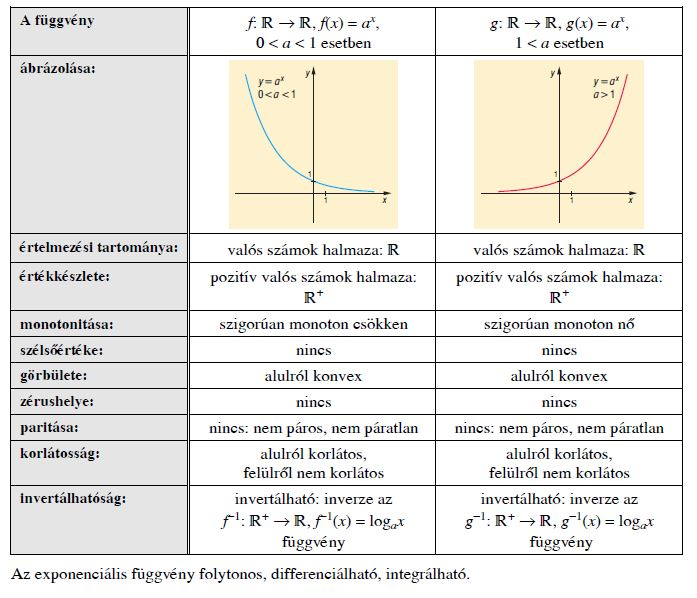
\includegraphics[width=\linewidth]{Exp}
	\end{figure}
\section{Logaritmusfüggvény}
	\begin{definition}
		Az $f:\mathbb{R}^+\longrightarrow\mathbb{R},\ f(x)=\log_ax,\ (a>0,\ a\ne1)$ függvényt logaritmusfüggvénynek nevezzük.
	\end{definition}
	\begin{figure}[H]
		\centering
		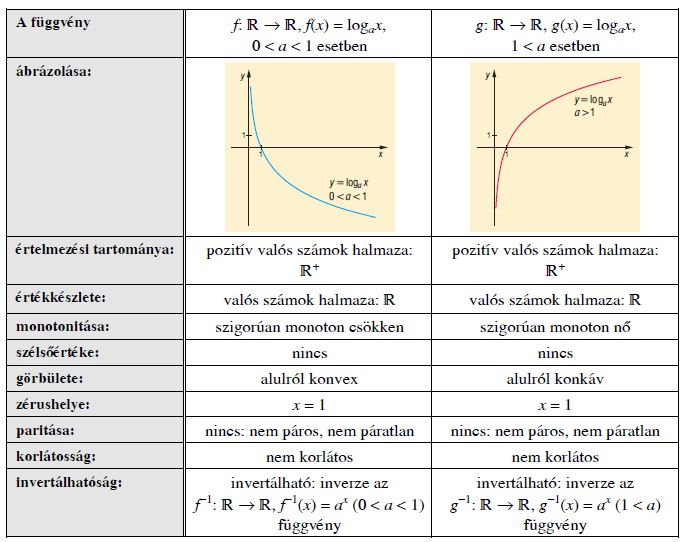
\includegraphics[width=\linewidth]{LogFv.JPG}
	\end{figure}
	Folytonos, differenciálható, integrálható
\section{Alkalmazások}
	\begin{itemize}
		\item Exponenciális egyenletek megoldása
		\item A levegő szerűsége a magassággal exponenciálisan csökken
		\item A Richter-skála logaritmus alapú
		\item Exponenciális függvény írja le a radioaktív izotópok bomlását
	\end{itemize}
\section{Matematikatörténet}
	\begin{outline}
		\1 Napier (XVI-XVII. század)
			\2 Logaritmus: matematikai számítások megkönnyítése
			\2 Csillagászati számításoknál volt hasznos
		\1 Bürgi (XVI-XVII. század)
			\2 Első logaritmustáblázat
	\end{outline}
\chapter{Egyenlet-megoldási módszerek}
\section{Egyenlet}
	\begin{definition}
		Az egyenlet bármely két egyenlőségjellel összekötött kifejezés. A kifejezésben szereplő
		változók az ismeretlenek.
	\end{definition}
	\begin{definition}
		Az alaphalmaz az ismeretlenek azon értékeinek halmaza, ahol az egyenletet vizsgáljuk,
		ahol a megoldásokat keressük.
	\end{definition}
	\begin{definition}
		Az egyenlet értelmezési tartománya az alaphalmaznak az a legbővebb részhalmaza,
		ahol az egyenletben szereplő kifejezések értelmezhetőek.
	\end{definition}
	\begin{definition}
		Az egyenletet igazzá tevő értékek az egyenlet megoldásai vagy gyökei.
	\end{definition}
	\begin{definition}
		Az alaphalmaz azon elemeinek halmaza, amelyekre az egyenlet igaz, az egyenlet megoldáshalmaza.
	\end{definition}
	\begin{definition}
		Az azonosság olyan egyenlet, amelynek a megoldáshalmaza megegyezik az egyenlet
		értelmezési tartományával.
	\end{definition}
\pagebreak
\section{Egyenlet-megoldási módszerek}
	\begin{outline}[enumerate]
		\1 Mérlegelv
			\2 Két oldal egyforma változtatása
			\2 Megoldáshalmaz nem változik, ha
				\3 az egyenlet mindkét oldalához ugyanazt a számot hozzáadjuk, vagy mindkét oldalából kivonjuk
				\3 az egyenlet mindkét oldalát ugyanazzal a 0-tól különböző számmal szorozzuk, osztjuk
		\1 Grafikus megoldás
			\2 Két oldal ábrázolása
			\2 Közös pont abszcisszája: megoldás
			\2 Hátrány: leolvasás pontatlan lehet
		\1 Szorzattá alakítás
			\2 Egyik oldal->szorzat
			\2 Másik oldal: 0
			\2 Szorzat=0<=>Valamelyik tényező=0
			\2 Pl.:$(x-2)x^2-(x-2)*x=0\implies(x-2)*2x=0$
		\1 Értelmezési tartomány vizsgálata
			\2 Ha $|D|=1$
				\3 Elem ellenőrzése
			\2 Ha $D=0$
				\3 Nincs megoldás
			\2 Pl.: $\sqrt{x-1}-\sqrt{1-x}=0$
				\3 $D={1}$
				\3 1 valóban megoldás
		\1 Értékkészlet vizsgálata
			\2 Két oldal értékkészletének metszetéből kerülhetnek ki a gyökök
			\2 Pl.:	$\frac{16}{3}x^4+\frac{1}{6x^2}=\sin(\pi x)$
				\3 $x\ne0$
				\3 Baloldal: deriválás
					\4 Minimum: $\pm\frac{1}{2}$-nél 1
				\3 Jobboldal: $\le1$
				\3 Bal és jobboldal = 1
				\3 Baloldal=$\pm\frac{1}{2}$
				\3 Jobboldalba helyettesítve csak a pozitív jó
		\1 Új ismeretlen bevezetése
			\2 Pl.: tg$^4(x)-5$tg$^2(x)+4=0\implies a^2-5a+4=0$
	\end{outline}
\section{Ekvivalencia}
	\begin{definition}
		Két egyenlet ekvivalens, ha alaphalmazuk és megoldáshalmazuk is azonos
	\end{definition}
	\begin{definition}
		Ekvivalens átalakítás olyan átalakítás, amit egyenletek megoldása közben végzünk, és az eredetivel ekvivalens egyenletet kapunk.
	\end{definition}
	\begin{outline}
		\1 Ekvivalens: mérlegelv
		\1 Nem ekvivalens: Négyzetre emelés
			\2 Szűkebb értelmezési tartomány: gyökvesztés lehet
			\2 Tágabb értelmezési tartomány: gyöknyerés lehet
	\end{outline}
\section{Gyökvesztés}
	Ismeretlent tartalmazó kifejezéssel való osztás. Például:
	\begin{align*}
		x^3+2x^2+x&=0\tag{Osztás nullával}\\
		x^2+2x+1&=0\\
		x=-1
	\end{align*}
	Helyesen:
	\begin{align*}
		x^3+2x^2+x&=0\\
		x*(x^2+2x)&=0\\
		x&=0\text{, vagy }\\
		x^2+2x=0&\implies x=-1
	\end{align*}
\section{Hamis gyök}
	Négyzetre emelés, például:
	\begin{align*}
		\sqrt{7-x}&=1-x\tag{Négyzetre emelés}\\
		7-x&=x^2-2x+1\\
		x=3&\vee x=-2
	\end{align*}
	Az $x=3$ nem megoldása az eredeti egyenletnek. Kiküszöbölhető közbülső feltétellel: $1-x\ge0$.
\section{Másodfokú egyismeretlenes egyenlet}
	\begin{definition}
		Másodfokú egyismeretlenes egyenlet $ax^2+bx+c=0$ alakra hozható, ahol $a,b,c\in\mathbb{R}$
	\end{definition}
	\begin{theorem}
		$ax^2+bx+c=0$ gyökei: $x_{1,2}=\frac{-b\pm\sqrt{b^2-4ac}}{2a}$, ahol $b^2-4ac\ge0$
	\end{theorem}
	\begin{proof}
		\begin{align*}
			ax^2+bx+c&=0\tag{$*4a$}\\
			4a^2x^2+4abx+4ac&=0\tag{Teljes négyzetté alakítás}\\
			(2ax+b)^2-b^2+4ac&=0\tag{$+b^2-4ac$}\\
			(2ax+b)^2&=b^2-4ac
		\end{align*}
		Mivel a baloldalon négyzetszám van, ami nem lehet negatív, $b^2-4ac$ sem lehet az, ha az lenne, a valós számok körében nincs megoldás. Ha $b^2-4ac\ge0$:
		\begin{align*}
			|2ax+b|&=\sqrt{b^2-4ac}\\
			2ax+b&=\pm\sqrt{b^2-4ac}\\
			2ax&=-b\pm\sqrt{b^2-4ac}\\
			x_{1,2}&=\frac{-b\pm\sqrt{b^2-4ac}}{2a}
		\end{align*}
	\end{proof}
	\begin{definition}
		Az $ax^2+bx+c=0$ másodfokú egyenlet diszkriminánsa $D=b^2-4ac$
	\end{definition}
	\begin{equation*}
	\text{Gyökök száma}=
	\begin{cases*}
		\text{Két különböző valós gyök}, & \text{ha} D>0\\
		\text{Kétszeres gyök}, &\text{ha} D=0\\
		\text{Nincs valós gyök},&\text{ha} D<0
	\end{cases*}
	\end{equation*}
	\begin{theorem}
		A másodfokú egyenlet $ax^2+bx+c=0$ gyöktényezős alakja, ha a diszkrimináns nemnegatív, és a két gyök $x_1$, $x_2$:
		\begin{equation*}
			a*(x-x_1)*(x-x_2)=0
		\end{equation*}
	\end{theorem}
	\begin{theorem}[Vi\`ete-formulák]
		$ax^2+bx+c$ alakú másodfokú egyenlet gyökei, és együtthatói közti összefüggések:
		\begin{align*}
			x_1+x_2&=-\frac{b}{a}\\
			x_1*x_2&=\frac{c}{a}
		\end{align*}
	\end{theorem}
\section{Alkalmazások}
	\begin{itemize}
		\item Egyenes, kör, parabola adott abszcisszájú vagy ordinátájú pontjának meghatározása
		\item Koszinusztételből oldalak kiszámítása
	\end{itemize}
	\begin{outline}
		\1 Vi\`ete ugrás (1988. IMO 6. feladat)
			\2  Indirekt bizonyítás
			\2 Legyen $a,b\in\mathbb{N}^+$, $(ab+1)|\left(a^2+b^2\right)$. Bizonyítsuk, hogy $\frac{a^2+b^2}{ab+1}$ teljes négyzet.
			\2 Indirekt bizonyítás
			\2 Legyen $k\in\mathbb{Z}^+$ úgy, hogy nem teljes négyzet. Tegyük fel, hogy: $\exists (a,\ b)\ k=\frac{a^2+b^2}{ab+1}$.
			\2 Legyenek $(A,\ B)\in\mathbb{Z}^+$, amikre: $k=\frac{A^2+B^2}{AB+1}$ úgy, hogy $A+B$ minimális. Az általánosság megszorítása nélkül feltehetjük, hogy $A\ge B$.
			\2 $A$ helyére $x$-et írva:
			\begin{align*}
				k&=\frac{x^2+B^2}{xB+1}\\
				kxB+k&=x^2+B^2\\
				x^2-(kB)x+(B^2-k)&=0
			\end{align*}
			\2 Tudjuk, hogy az egyik gyök: $x_1=A$. A másik gyökre igaz, hogy:
			\begin{equation*}
				x_2=kB-A\wedge x_2=\frac{B^2-k}{A}
			\end{equation*}
			\2 Első kifejezés miatt: $x_2\in\mathbb{Z}$. A másodikból: $x_2\ne0$, mert $k$ nem teljes négyzet
			\2 $\frac{x_2^2+B^2}{x_2B+1}=k>0\implies x_2>0$, mert a számláló, és a tört értéke pozitív, így a nevezőnek is pozitívnak kell lennie: $x_2B+1>0\implies x_2B>-1$. Mivel $B$ pozitív egész, $x_2$ nem lehet negatív.
			\2[] 
			\begin{align*}
				A&\ge B\tag{Mivel mindkét oldal pozitív}\\
				A^2&\ge B^2\\
				A^2-k&\ge B^2-k\tag{Mivel $A>0$}\\
				A-\frac{k}{A}&\ge \frac{B^2-k}{A}\\
				\frac{B^2-k}{A}&\le A-\frac{k}{A}<A\\
				x_2&<A\\
				x_2+B&<A+B
			\end{align*}
			\2 Ez azonban ellentmond $(A,\ B)$ minimalitásának
	\end{outline}
\section{Matematikatörténet}
	\begin{outline}
		\1 Vi\`ete (XVI. század)
			\2 Másodfokú egyenlet gyökök és együtthatók közti összefüggések
		\1 Cardano (XVI. század)
			\2 Harmadfokú egyenlet megoldóképlete
				\3 Casus irreducibilis, ha 3 különböző valós gyök van
			\2 Negyedfokú egyenlet visszavezetése harmadfokúra
		\1 Abel (XIX. század)
			\2 Negyedfokúnál magasabb fokú egyenletekre nincs általános megoldóképlet
	\end{outline}
\chapter{Statisztika}
\section{Adatsokaságok jellemzői}
	A statisztika feladatai közé tartozik, hogy bizonyos egyedek meghatározott tulajdonságairól
	tájékozódjék, majd a szerzett (általában számszerű) adatokat feldolgozza, elemzi.
	\begin{definition}
		Az	elemzéshez összegyűjtött adatok halmazát adatsokaságnak, mintának, a meghatározott tulajdonságot ismérvnek, változónak nevezzük.
	\end{definition}
	\begin{definition}
		A sokaság elemeinek az ismérv szerinti tulajdonságát statisztikai adatnak, az adatsokaság elemeinek számát a sokaság méretének nevezzük.
	\end{definition}
\section{A leíró statisztika jellemzői}
	\begin{outline}
		\1 Tömegesen előforduló jelenségek(ből nyert adatok) vizsgálata
		\1 Adatok összegyűjtése
			\2 Ha vizsgálandó egyedek száma nagy
			\2 Adatsokaság részhalmazát vizsgáljuk
				\3 Mintavétel
				\3 Mintából következtetés a sokaságra
			\2 Reprezentatív mintavétel:
				\3 Tulajdonság előfordulása mintában közelíti a sokaságban való előfordulást
			\2 Véletlenszerű mintavétel:
				\3 Minden elem ugyanakkora valószínűséggel->minta
	\end{outline}
	\begin{definition}
		Az egyes adatok előfordulásának a száma a gyakoriság.
	\end{definition}
	\begin{definition}[Relatív gyakoriság]
		A gyakoriság osztva az adatok számával
	\end{definition}
	\begin{outline}
		\1 Adatok megadása: lehet táblázat
			\2 Nagyobb adathalmazok tömör ábrázolása
			\2 Gyakorisági táblázat: Lehetséges adatok, hozzá tartozó gyakoriságok
		\1 Osztályok
			\2 Nagy méretű adatsokaság, vagy sok különböző érték közel azonos gyakorisággal
			\2 Egymáshoz közeli értékek összevonása
			\2 Diszjunktak, hézagmentesek
	\end{outline}
\section{Diagramok}
	\begin{outline}
		\1 Adatok grafikus megjelenítése
		\1 Oszlopdiagram:
			\2 Adatok egymáshoz való viszonya
			\2 Nem célszerű, ha
				\3 Van 1-2 kiugró érték
				\3 Adatok közötti eltérés nagyon kicsi
			\2 Víszintes tengely: adatfajtáknak megfelelő intervallumok
				\3 Ezek fölé téglalapok
				\3 Területük arányos gyakorisággal
		\1 Hisztogram
			\2 Gyakorisági eloszlás oszlopdiagramon
			\2 Oszlopok hézagmentesen
		\1 Sávdiagram
			\2 Fordított oszlopdiagram
		\1 Kördiagram
			\2 Részadatok egészhez való viszonya
			\2 Alkalmas \%-os adatok ábrázolására
				\3 360\degree: 100\%
			\2 Nem célszerű, ha sok az adat
		\1 Vonaldiagram
			\2 Koordináta-rendszerben pontként
			\2 Töröttvonal köti össze
			\2 Időbeli változás
			\2 Gyakoriságok vonaldiagramja: gyakorisági poligon.
	\end{outline}
\section{Statisztikai mutatók}
	\subsection{Középértékek}
	\begin{outline}
		\1 Adatsokaságokat csak leegyszerűsítve lehet jellemezni
			\2 Középértékek: egy számmal írnak le egy adathalmazt
			\2 Előny: valamilyen tulajdonság jó megjelenítése
			\2 Hátrány: nem nyújtanak képet egyes adatokról
	\end{outline}
\pagebreak
	\begin{outline}
		\1[] \begin{definition}[Módusz]
				Egy adatsokaságban a leggyakrabban előforduló adat.
			\end{definition}
			\2 Ha 1 db van: egymóduszú adatsokaság
				\3 Különben többmóduszú
			\2 Előny: Könnyű meghatározni
			\2 Hátrány: Csak akkor használható jellemzés, ha a többi adathoz képest sokszor fordul elő
		\1[] \begin{definition}[Átlag (számtani közép)]
				Az adatok összegének és az adatok számának hányadosa, jele: $\overline{x}$.
			\end{definition}
			\2 $\sum$Nagyobb adatoktól vett eltérések$=\sum$Kisebb adatoktól vett eltérések
			\2 Hátrány: egy kiugró adat eltorzíthatja
		\1[] \begin{definition}[Medián]
			Páratlan számú adat esetén nagyság szerinti sorrendben a középső adat. Páros számú adat esetén a két középső adat átlaga
		\end{definition}
			\2 Összes adat fele $\le$ Medián
			\2 Összes adat fele $\ge$ Medián
			\2 Adatoktól mért távolságok összege minimális
			\2 Előny: valóban középérték
				\3 Ugyanannyi adat nagyobb, mint amennyi kisebb
	\end{outline}
	\subsection{Szóródás jellemzői}
	\begin{outline}
		\1[] \begin{definition}[Terjedelem]
				Legnagyobb és legkisebb adat különbsége
			\end{definition}
			\2 Minél kisebb, annál jobban jellemzi a mintát
		\1[] \begin{definition}[Variancia (szórásnégyzet)]
				Adatok átlagtól való eltérések négyzetének átlaga
			\end{definition}
		\1[] \begin{definition}[Szórás]
				Szórásnégyzet négyzetgyöke:
				\begin{equation*}
					\sigma=\sqrt{\frac{\sum_{i=1}^{n}\left(x_i-\overline{x}\right)^2}{n}}
				\end{equation*}
			\end{definition}
			\2 Megmutatja, adatok mennyire térnek el az átlagtól
			\2 Minél kisebb, átlag annál jobban jellemez
		\1[] 
		\begin{theorem}[Bessel korrekció]
			Ha $s^2$ a minta varianciája, akkor az adatsokaság varianciáját jobban jellemzi: $s^2*\frac{n}{n-1}$.
		\end{theorem}
	\end{outline}
\section{Pozitív számok nevezetes közepei}
	\begin{definition}
		$a_1,a_2,\dots,a_n$ nemnegatív számok
		\begin{itemize}
			\item Aritmetikai (számtani) közepe: 
			\begin{equation*}
				A=\frac{\sum_{i=1}^n a_i}{n}
			\end{equation*}
			\item Geometriai (mértani) közepe:
			\begin{equation*}
				G=\sqrt[n]{\prod_{i=1}^n a_i}
			\end{equation*}
			\item Kvadratikus (négyzetes) közepe:
			\begin{equation*}
				Q=\sqrt{\frac{\sum_{i=1}^na_i^2}{n}}
			\end{equation*}
			\item Harmonikus közepe:
			\begin{equation*}
				H=\frac{n}{\sum_{i=1}\frac{1}{a_i}},\text{ ha } a_i>0
			\end{equation*}
		\end{itemize}
	\end{definition}
	\begin{theorem}[Közepek közötti összefüggés]
		\begin{equation*}
		H\le G\le A\le Q
		\end{equation*}
		Egyenlőség csak akkor áll fenn, ha $\forall i,j\ a_i=a_j$
	\end{theorem}
	\begin{theorem}
		Két nemnegatív valós szám esetén $\sqrt{a*b}\le \frac{a+b}{2}$
	\end{theorem}
	\begin{proof}
		Mivel az egyenlőtlenség mindkét oldala nemnegatív, a négyzetre emelés ekvivalens átalakítás.
		\begin{gather*}
			\sqrt{ab}\le\frac{a+b}{2}\Leftrightarrow ab\le\frac{a^2+2ab+b^2}{4}\Leftrightarrow 
			4ab\le a^2+2ab+b^2\Leftrightarrow 0\le a^2-2ab+b^2\Leftrightarrow\\
			\Leftrightarrow 0\le (a-b)^2
		\end{gather*}
		Az utolsó egyenlőtlenség igaz, és mivel mindig ekvivalens átalakításokat végeztünk, az eredeti is igaz.
	\end{proof}
\section{Nevezetes közepek alkalmazása szélsőérték-feladatokban}
	\subsection{Összeg állandósága esetén szorzat maximalizálása.}
	Azon téglatestek közül, amelyek éleinek összege 60 cm, melyiknek a térfogata maximális?
	
	Legyenek a téglatest élei: $a,\ b$ és $c$. Ekkor a térfogata: $V=a*b*c$, az élek összege: $4*(a+b+c)=60$. Ebből $a+b+c=15$. A számtani és mértani közép közötti egyenlőtlenségből:
	\begin{gather*}
		\frac{a+b+c}{3}\ge\sqrt[3]{abc}\implies \left(\frac{a+b+c}{3}\right)^3\ge abc\implies \left(\frac{15}{3}\right)^3\ge abc\implies 5^3\ge abc\implies\\
		\implies 125\ge V
	\end{gather*}
	Mivel egyenlőség csak $a=b=c$ esetén teljesül, így a térfogat az 5 cm élű kocka esetén maximális.
	\subsection{Szorzat állandósága esetén összeg minimalizálása}
	Azon téglalapok közül, amelyeknek a területe $100 cm^2$, melyiknek a kerülete minimális?
	Legyenek a téglalap oldalai $a$ és $b$. Ekkor a területe: $T=ab=100$, kerülete: \\
	$K=2(a+b)$, amiből $\frac{K}{4}=\frac{a+b}{2}$. A számtani és mértani közép közti egyenlőtlenséget kihasználva:
	\begin{equation*}
		\frac{a+b}{2}\ge\sqrt{ab}\implies\frac{K}{4}\ge\sqrt{100}\implies\frac{K}{4}\ge 100\implies K\ge 40
	\end{equation*}
	Mivel egyenlőség csak $a=b$ esetén teljesül, így kerület a 10 cm oldalú négyzet esetén minimális.
\section{Alkalmazások}
	\begin{outline}
		\1 Statisztika
			\2 Közvélemény-kutatások
			\2 Gazdasági mutatók
		\1 Nevezetes közepek
			\2 Négyzetes közép: statisztikai szórás kiszámítása
			\2 Harmonikus közép: átlagsebesség meghatározása
	\end{outline}
\section{Matematikatörténet}
	\begin{outline}
		\1 William Sealy Gosset (Student, XIX-XX. század)
			\2 $t$ eloszlás
			\2 Fizikai mérések véletlen hibájának becslése
			\2 Konfidenciaintervallum: $t^*\frac{s}{\sqrt{n}}$
		\1 Friedrich Bessel (XVIII-XIX. század)
			\2 Bessel korrekció
	\end{outline}
\chapter{Számsorozatok}
\section{Számsorozat}
	\begin{definition}
		A számsorozat olyan függvény, amelynek értelmezési tartománya a pozitív egész számok
		halmaza, értékkészlete pedig valamilyen számhalmaz. Az $a_1,\dots,\ a_n$ tagokból álló sorozatot \{$a_n$\}-nel vagy ($a_n$)-nel jelöljük. A sorozat n-edik tagja: $a_n$.
	\end{definition}
	\begin{outline}
		\1 Megadásuk
			\2 Függvényszerűen: $f:\mathbb{N}^+\longrightarrow\mathbb{R},\ x\mapsto x^2$
			\2 Az n-edik általános tagot előállító formulával: $\{a_n\}=3*2^n$
			\2 Az elemeit egyértelműen meghatározó utasítással: $\{a_n\}=\{2^n \text{ utolsó számjegye}\}$
			\2 A sorozat tagjaival: $3,\ 6,\ 9,\dots$
			\2 Rekurzívan: $a_1=1,\ a_2=2,\ a_n=a_{n-1}+a_{n-2},$ ha $n\ge3$
	\end{outline}
\section{Sorozatok tulajdonságai}
	\begin{definition}
		Az $\{a_n\}$ sorozat szigorúan monoton növekvő, ha $\forall n\in\mathbb{Z}^+\ a_n<a_{n+1}$.
	\end{definition}
	\begin{definition}
		Az $\{a_n\}$ sorozat szigorúan monoton csökkenő, ha $\forall n\in\mathbb{Z}^+\ a_n>a_{n+1}$.
	\end{definition}
	\begin{outline}
		\1 Ha csak monotonitás: megengedett egyenlőség is
		\1 Keresése:
			\2 $a_{n+1}-a_n$
			\2 $\frac{a_{n+1}}{a_n}$
				\3 Minden tag pozitív
	\end{outline}
	\begin{definition}
		Egy $\{a_n\}$ sorozatnak $K$ felső korlátja, ha $\forall n\in\mathbb{N}^+\ a_n\le K$. Ilyenkor a sorozatot felülről korlátosnak nevezzük.
	\end{definition}
	\begin{definition}
		Egy $\{a_n\}$ sorozatnak $k$ alsó korlátja, ha $\forall n\in\mathbb{N}^+\ a_n\ge k$. Ilyenkor a sorozatot alulról korlátosnak nevezzük.
	\end{definition}
	\begin{definition}
		Egy sorozat korlátos, ha alulról és felülről is korlátos.
	\end{definition}
	\begin{definition}
		Felülről korlátos sorozat legkisebb felső korlátját a sorozat felső határának (szuprémum, $\sup$), alulról korlátos sorozat legnagyobb alsó korlátját a sorozat alsó határának nevezzük (infimum, $\inf$).
	\end{definition}
	\begin{theorem}
		Felülről korlátos sorozatnak van felső határa, alulról korlátos sorozatnak van alsó határa.
	\end{theorem}
	\begin{theorem}
		Végtelen sok egymásba skatulyázott, zárt intervallumnak van közös pontja. Ha az intervallumok hossza 0-hoz tart, akkor pontosan egy közös pont van.
	\end{theorem}
	\begin{definition}
		Az \{$a_n$\} sorozat konvergens és határértéke az $A$ szám, ha
		\begin{equation*}
			\forall\epsilon>0\ \exists N\in\mathbb{Z}^+\ n>N\implies|a_n-A|<\epsilon
		\end{equation*}
		Jelölése: $\lim\limits_{n\rightarrow\infty}a_n=A$, vagy $a_n\rightarrow A$.
	\end{definition}
	\begin{definition}
		Az olyan sorozatokat, amelyeknek nincs határértéke, divergens sorozatoknak nevezzük.
	\end{definition}
	\begin{theorem}[]
		Konvergens sorozatok tulajdonságai:
		\begin{itemize}
			\item Csak egy határértéke van
			\item Korlátos
			\item Ha monoton és korlátos, akkor konvergens. Határérték növekedés esetén felső, csökkenés esetén alsó határ
			\item Rendőr-elv: $\left(\left(\left(\forall n\in\mathbb{N}^+\ a_n\le b_n\le c_n\right)\wedge a_n\rightarrow A\right)\wedge c_n\rightarrow A\right)\implies b_n\rightarrow A$
		\end{itemize}
	\end{theorem}
\section{Műveletek konvergens sorozatokkal}
	\begin{outline}
		\1 $\{a_n\},\ \{b_n\}$ konvergens, és $a_n\rightarrow A, b_n\rightarrow B$
			\2 $a_n\pm b_n\rightarrow A\pm B$
			\2 $a_n*b_n\rightarrow A*B$
			\2 $c*a_n\rightarrow c*A$, ahol $c\in\mathbb{R}$
			\2 $\frac{a_n}{b_n}\rightarrow\frac{A}{B}$, ahol $b_n\ne0,\ B\ne0$
	\end{outline}
\section{Számtani sorozat}
	\begin{definition}
		Azt a számsorozatot, amelyben a második tagtól kezdve bármely tag és a közvetlenül
		előtte álló tag különbsége állandó, számtani sorozatnak nevezzük. Ez a különbség a differencia, jele $d$.
		\begin{equation*}
		\begin{cases*}
			\text{Szigorúan monoton nő, és alulról korlátos ha} & d>0\\
			\text{Konstans, ha} & d=0\\
			\text{Szigorúan monoton csökken, és felülről korlátos, ha} & d<0
		\end{cases*}
		\end{equation*}
	\end{definition}
	\begin{theorem}
		Ha egy számtani sorozat első tagja $a_1$, differenciája $d$, akkor n-edik tagja $a_n=a_1+(n-1)*d$.
	\end{theorem}
	\begin{theorem}
		A számtani sorozat első n tagjának összege ($S_n$) az első és az n-edik tag számtani közepének n-szeresével egyenlő: $S_n=\frac{a_1+a_n}{2}*n$
	\end{theorem}
	\begin{proof}
		Az összeget felírjuk az 1., majd az n-edik tagtól kiindulva:
		\begin{align*}
			S_n&=a_1+\dots+a_k+\dots+a_n=a_1+\dots+(a_1+(k-1)d)+\dots+(a_1+(n-1)d)\\
			S_n&=a_n+\dots+a_{n-k+1}+\dots+a_1=(a_1+(n-1)d)+\dots+(a_1+(n-k)d)+\dots+a_1\\
		\end{align*}
		A kettőt összeadva:
		\begin{align*}
			2S_n&=2a_1+(n-1)d+\dots+2a_1(n-1)d+\dots+2a_1+(n-1)d=n*(2a_1+(n-1)d)\\
			S_n&=\frac{2a_1+(n-1)d}{2}*n=\frac{a_1+a_n}{2}*d\qedhere
		\end{align*}
	\end{proof}
	\begin{theorem}
		$S_n$ másik alakja:
		\begin{equation*}
			S_n=\frac{2a_1+(n-1)d}{2}*n
		\end{equation*}
	\end{theorem}
	\begin{theorem}
		Tetszőleges elem a tőle szimmetrikusan elhelyezkedőknek a számtani közepe:
		\begin{equation*}
			a_n=\frac{a_{n-k}+a_{n+k}}{2}
		\end{equation*}
	\end{theorem}
\section{Alkalmazások}
	\begin{itemize}
		\item Irracionális kitevőjű hatvány fogalma sorozat határértékével.
		\item Speciális függvények közelítése polinomokkal, pl.:
		\begin{align*}
			\sin(x)&=x-\frac{x^3}{3!}+\frac{x^5}{5!}-\dots=\sum_{n=0}^{\infty} \left(\frac{(-1)^n*x^{2n-1}}{(2n-1)!}\right)\\
			\cos(x)&=1-\frac{x^2}{2!}+\frac{x^4}{4!}-\dots=\sum_{n=0}^{\infty} \left(\frac{(-1)^n*x^{2n}}{(2n)!}\right)\\
		\end{align*}
	\end{itemize}
\section{Matematikatörténet}
	\begin{outline}
		\1 Euler (XVIII. század)
			\2 $\lim\limits_{n\to\infty} \left(1+\frac{1}{n}\right)^n=e$ határérték bevezetése
		\1 Cauchy (XVIII-XIX. század)
			\2 Analízis alapvető fogalmainak (konvergencia, sorozat, határérték) szilárd alapokra fektetése
	\end{outline}
\chapter{Mértani sorozat}
\section{Mértani sorozat}
	\begin{definition}
		A számsorozat olyan függvény, amelynek értelmezési tartománya a pozitív egész számok
		halmaza, értékkészlete pedig valamilyen számhalmaz. Az $a_1,\dots,\ a_n$ tagokból álló sorozatot \{$a_n$\}-nel vagy ($a_n$)-nel jelöljük. A sorozat n-edik tagja: $a_n$.
	\end{definition}
	\begin{definition}
		Azt a számsorozatot, amelyben a második tagtól kezdve bármely tag és a közvetlenül
		előtte álló tag hányadosa állandó, mértani sorozatnak nevezzük. Ez a hányados a kvóciens,
		jele $q$. A definíció kizárja, hogy a sorozat bármely eleme 0 legyen, továbbá a kvóciens sem lehet 0.
	\end{definition}
	\begin{theorem}
		Ha egy mértani sorozat első tagja $a_1$, hányadosa $q$, akkor n-edik tagja $a_n=a_1*q^{n-1}$
	\end{theorem}
	\begin{theorem}
		A mértani sorozat első n tagjának összege:
			\begin{equation*}
			S_n=
			\begin{cases*}
			n*a_1,& ha $q=1$\\
			a_1*\frac{q^n-1}{q-1},& ha $q\neq 1$
			\end{cases*}
		\end{equation*}
	\end{theorem}
	\begin{proof}
		Ha $q=1$, akkor a sorozat minden tagja $a_1$, így: $S_n=\sum_{i=1}^{n} a_1=n*a_1$. Ha $q\ne1$, akkor:
		\begin{align*}
			S_n&=a_1+a_1q+\dots+a_1q^{k-1}+\dots+a_1q^{n-1}\\
			q*S_n&=a_1q+a_1q^2+\dots+a_1q^{k}+\dots+a_1q^n\\
			S_n*q-S_n&=a_1*q^n-a_1\tag{Két egyenletet kivonva egymásból}\\
			S_n(q-1&=a_1*(q^n-1)\\
			S_n&=a_1*\frac{q^n-1}{q-1}\tag{Mindkét oldal osztva $q-1\ne0$-val}
		\end{align*}
	\end{proof}
	\begin{theorem}
		Bármely elem négyzete egyenlő a tőle szimmetrikusan elhelyezkedő tagok szorzatával:
		\begin{equation*}
			a_n^2=a_{n-k}*a_{n+k}
		\end{equation*}
	\end{theorem}
	\begin{theorem}
		Pozitív tagú sorozatnál bármely elem a tőle szimmetrikusan elhelyezkedő elemek mértani
		közepe:
		\begin{equation*}
			a_n=\sqrt{a_{n-k}*a_{n+k}}\text{, ha }\forall n\in\mathbb{N}^+\ a_n>0
		\end{equation*}
	\end{theorem}
	\begin{theorem}[Mértani sorozat konvergenciája]
		\begin{equation*}
			\begin{cases*}
				a_n\longrightarrow a_1,& ha $q=1$\\
				a_n\longrightarrow 0,& ha $|q|<1$\\
				\{a_n\}\text{ divergens},& ha $q=-1\vee|q|>1$
			\end{cases*}
		\end{equation*}
	\end{theorem}
\section{Végtelen mértani sor}
	\begin{definition}
		Legyen $\{a_n\}$ egy számsorozat A $\sum_{i=1}^\infty a_i$ összeget végtelen sornak nevezzük.
	\end{definition}
	\begin{definition}
		Ha a $\sum_{i=1}^\infty a_i$ végtelen sorban \{$a_i$\} sorozat egy mértani sorozat, akkor a végtelen sort mértani sornak nevezzük.
	\end{definition}
	\begin{definition}
		A sor összegén a $\lim\limits_{n\to\infty} S_n=\lim\limits_{n\to\infty} \sum_{i=1}^n a_i$ határértéket értjük, amennyiben létezik.
	\end{definition}
	\begin{theorem}
		Ha egy mértani sorban $|q|<1$, akkor a mértani sor konvergens, és összege $S=\frac{a_1}{1-q}$, ha $|q|\ge1$, akkor nem konvergens.
	\end{theorem}
\section{Kamatszámítás}
	\begin{outline}
		\1 Kamat: tőke használatáért járó díj
			\2 Tőke: Kölcsönadott, letétbe helyezett pénz
			\2 Nagysága: tőke százalékában (kamatláb)
			\2 Kamattényező: 
				\3 Értéknövekedés: $q=1+\frac{p}{100}$
				\3 Értékcsökkenés: $q=1-\frac{p}{100}$
		\1 Kamatos kamat: Kamatozás után, kamat+tőke kamatozik
			\2 Mértani sorozat
				\3 Van nulladik tag (a)
			\2 $a$ összeg $p\%$-ot kamatozik évente, akkor az $n$-edik év végére az összeg:\\ $a_n=a*\left(1+\frac{p}{100}\right)^n$
			\2 Éves kamatláb $p\%$, akkor
				\3 Havi: $\sqrt[12]{1+\frac{p}{100}}$
				\3 Napi: $\sqrt[365]{1+\frac{p}{100}}$
	\end{outline}
\section{Gyűjtőjáradék}
	\begin{outline}
		\1 Alapösszeget időközönként azonos összeggel növelünk, a teljes összeg kamatozik
		\1 Minden év elején $a$ összeget teszünk be, ez $p\%$-al kamatozik.
			\2 $q=1+\frac{p}{100}$
			\2 n-edik év végén: mértani sorozat első n elemének összege, ahol $a_1=aq$. $S_n=a*q\frac{q^n-1}{q-1}$
	\end{outline}
\section{Törlesztőrészlet}
	\begin{outline}
		\1 Hitelt egyenlő időközönként ugyanakkora összeggel fizetünk vissza, mindig a fennálló tartozásra fizetjük a kamatos kamatot
		\1 $n$ évre $S_n$ nagyságú hitelt évi $p\%$-os kamatra veszünk fel, minden évben $a$ összeget törlesztünk.
			\2 $n$-edik év végén befizetések kamatokkal megnövelt értéke egyenlő a kölcsön $n$ év alatt $p\%$-os kamatozással megnőtt értékével. Ha $q=1+\frac{p}{100}$, akkor $S_n*q^n=a*\frac{q^n-1}{q-1}$.
	\end{outline}
\section{Exponenciális folyamatok}
	\begin{outline}
		\1 Időben növekedés: $N_t=N_0*e^{\lambda t}$, csökkenés: $N_t=N_0*e^{-\lambda t}$.
			\2 $N_0$ - kezdeti mennyiség, $N_t$ - t időpontbeli mennyiség, $\lambda$ - folyamatra jellemző paraméter
		\1 Minél nagyobbak, annál gyorsabban növekednek. Változást exponenciális függvény írja le.
		\1 Föld túlnépesedése
			\2 Matematikai modell: 1837 óta minden évben 1,1\%-al nő: $N_t=1*1,011^t$.
				\3 Kb. 63 évente duplázódik
			\2 Ugyanannyi időközönként egyre nagyobb számmal nő népesség
			\2 Rendelkezésre álló erőforrások nem tudnak lépést tartani
			\2 Vagy életfeltételek romlása, vagy népesség növekedése csökken
		\1 Diszkrét exponenciális növekedés: kamatos kamat
		\1 Diszkrét exponenciális csökkenés: tárgyak értékcsökkenése
			\2 Évi $p\%$-os: $a_n=a*\left(1-\frac{p}{100}\right)^n$
		\1 Térbeli: sugárzások elnyelődése homogén közegben
	\end{outline}
\section{Alkalmazások}
	\begin{outline}
		\1 Végtelen szakaszos tizedestörtek közönséges tört alakra hozása: konvergens mértani sor tulajdonságai
		\1 Exponenciális függvény:
			\2 Radioaktív izotópok bomlási egyenletei
			\2 Oldódás folyamata
			\2 Kondenzátor feltöltődésének, kisülésének folyamata
	\end{outline}
\section{Matematikatörténet}
	\begin{outline}
		\1 Beidomandi (1300-as évek)
			\2 Mértani sorozat összegképlete
		\1 Koch (XIX-XX. század)
			\2 Koch-görbe: Szabályos háromszög oldalainak harmadolása, középső harmad fölé kifele szabályos háromszög. Ezen háromszögön újból harmadolás. Kerület, terület kiszámítása mértani sor összegeként:
				\3 $K=\infty$
				\3 $T=\frac{2a^2\sqrt{3}}{5}$
			\2[] \begin{figure}[H]
				\centering
				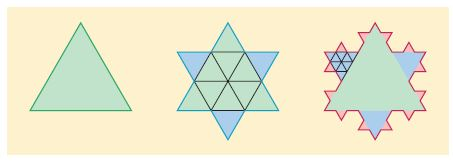
\includegraphics[width=0.8\linewidth]{Koch}
			\end{figure}
	\end{outline}
\chapter{Deriválás}
\section{Függvény fogalma, értelmezési tartomány, értékkészlet}
	\begin{definition}
		Legyen $A$ és $B$ két nem üres halmaz. Azt mondjuk, hogy megadunk egy $A$ halmazon értelmezett $B$-beli értéket felvevő függvényt, ha $A$ minden eleméhez hozzárendeljük $B$ egy elemét. Jele: $f:\ A\mapsto B$
	\end{definition}
	\begin{definition}
		Értelmezési tartománynak nevezzük az $A$ halmazt. Jele: $D_f$
	\end{definition}
	\begin{definition}
		Értékkészlet a $B$ halmaz azon elemeiből álló halmaz, amelyek a hozzárendelésnél fellépnek. Jele: $R_f$
	\end{definition}
	\begin{definition}
		Ha $c\in D_f$, akkor a $c$ helyen felvett függvényértéket $f(c)$-vel jelöljük, ez a helyettesítési, vagy függvényérték.
	\end{definition}
	\begin{definition}
		Ha az értelmezési tartomány és az értékkészlet is számhalmaz, akkor a függvényt grafikonon tudjuk szemléltetni. A grafikon az $(x;f(x))$ pontok halmaza.
	\end{definition}
\section{Függvénytulajdonságok}
	\subsection{Lokális függvénytulajdonságok}
	Zérushely, monotonitás, lokális szélsőérték, görbület, inflexió, pontbeli folytonosság.
	\begin{definition}[Zérushely]
		Az értelmezési tartomány azon $x_0$ eleme, ahol a függvény értéke 0. $f(x_0)=0$.
	\end{definition}
	\begin{definition}[Monotonitás]
		Az $f$ függvény az értelmezési tartományának egy intervallumában monoton nő, ha az intervallum minden olyan $x_1, x_2$ helyén, amelyre $x_1<x_2$, $f(x_1)\le f(x_2)$.
		
		Az $f$ függvény az értelmezési tartományának egy intervallumában monoton csökken, ha az intervallum minden olyan $x_1, x_2$ helyén, amelyre $x_1<x_2$, $f(x_1)\ge f(x_2)$.
		
		Ha az egyenlőtlenségben az egyenlőség nincs megengedve, akkor szigorú monotonitásról
		beszélünk.
	\end{definition}
	\begin{definition}[Lokális szélsőérték]
		Az $f$ függvénynek az $x_0\in D_f$ helyen lokális maximuma van, ha az $x_0$-nak van olyan $I$ környezete, amelynek minden $x\in D_f$ pontjában $f(x)\le f(x_0)$. Az $x_0$ helyet lokális maximumhelynek nevezzük.
		
		Az $f$ függvénynek az $x_0\in D_f$ helyen lokális minimuma van, ha az $x_0$-nak van olyan $I$ környezete, amelynek minden $x\in D_f$ pontjában $f(x)\ge f(x_0)$. Az $x_0$ helyet lokális minimumhelynek nevezzük.
	\end{definition}
	A monotonitás és a szélsőérték definíciójából következik, hogy ahol a függvény monotonitást
	vált, ott lokális szélsőértéke van.
	\begin{definition}[Görbület]
		A függvényt egy intervallumban konvexnek nevezzük, ha az intervallum bármely két $x_1,x_2$ pontjára teljesül: $f\left(\frac{x_1+x_2}{2}\right)\le\frac{f(x_1)+f(x_2)}{2}$. Ha az egyenlőtlenség fordított irányú, akkor a függvény konkáv az adott intervallumon.
	\end{definition}
	\begin{definition}[Inflexiós pont]
		A függvénygörbének azt a pontját, ahol a görbe konvexből konkávba, vagy
		konkávból konvexbe megy át, inflexiós pontnak nevezzük.
	\end{definition}
	\begin{definition}[Pontbeli folytonosság]
		Az $f$ függvény értelmezési tartományának egy $x_0$ pontjában folytonos, ha létezik $x_0$ pontban határértéke, és ez megegyezik a helyettesítési értékével, azaz: $f(x_0)=\lim\limits_{x\to x_0}f(x)$
	\end{definition}
	\subsection{Globális függvénytulajdonságok}
	Értelmezési tartomány, értékkészlet, globális (abszolút) szélsőérték, paritás, periodikusság, intervallumbeli folytonosság, korlátosság.
	\begin{definition}[Globális szélsőérték]
		Az $f$ függvénynek az $x_0\in D_f$ helyen globális maximuma van, ha $\forall x\in D_f\ f(x)\le f(x_0)$. Az $x_0$ helyet globális maximumhelynek nevezzük.
		
		Az $f$ függvénynek az $x_0\in D_f$ helyen globális minimuma van, ha $\forall x\in D_f\ f(x)\ge f(x_0)$. Az $x_0$ helyet globális maximumhelynek nevezzük.
	\end{definition}
	\begin{definition}[Paritás]
		Az $f$ függvény páros, ha \\
		\begin{equation*}
			x\in D_f\implies (-x)\in D_f\wedge\forall x\in D_f f(x)=f(-x)
		\end{equation*}
		
		Az $f$ függvény páratlan, ha \begin{equation*}
			x\in D_f\implies (-x)\in D_f\wedge\forall x\in D_f f(x)=-f(-x)
		\end{equation*}
	\end{definition}
	Páros függvények grafikonja tengelyesen szimmetrikus az y tengelyre (pl.: $x^{2n},|x|,\cos x$). Páratlan függvények grafikonja középpontosan szimmetrikus az origóra (pl.: $x^{2n+1},\frac{1}{x},\sin x,\text{tg} x$)
	\begin{definition}[Periodikusság]
		Az $f$ függvény periodikus, ha 
		\begin{equation*}
			\exists p\in\mathbb{R}\ p\ne0\ x\in D_f\implies (x+p)\in D_f\wedge\forall x\in D_f\ f(x)=f(x+p)
		\end{equation*}
		$p$ a függvény periódusa (pl.: trigonometrikus függvények, törtrész függvény)
	\end{definition}
	\begin{definition}[Intervallumbeli folytonosság]
		Az $f$ függvény egy nyílt intervallumban folytonos, ha az intervallum minden pontjában folytonos.
	\end{definition}
	Pl.: Folytonos: $x^n, \log_a x, a^x, \sin x, \cos x$. Nem folytonos: egészrész, $\frac{1}{x}$ tg $x$, ctg $x$.
	\begin{definition}[Korlátosság]
		Az $f$ függvény felülről korlátos az értelmezési tartományának egy $I$ intervallumában, ha $\exists K\ \forall x\in I\ f(x)\le K$. Egy függvény felső korlátai közül a legkisebbet felső határnak (szuprémumnak) nevezzük.
		
		Az $f$ függvény alulról korlátos az értelmezési tartományának egy $I$ intervallumában, ha $\exists k\ \forall x\in I\ f(x)\ge k$. Egy függvény alsó korlátai közül a legnagyobbat felső határnak (szuprémumnak) nevezzük.
		
		Egy függvény korlátos, ha alulról és felülről is korlátos.
	\end{definition}
\section{Differenciálszámítás}
	\begin{definition}
		Legyen $f$ egy $]a,b[$ intervallumon értelmezett függvény és $x_0$ az értelmezési tartomány egy pontja. Ekkor a $g(x)=\frac{f(x)-f(x_0)}{x-x_0}$ függvényt az $f$ függvény $x_0$ pontjához tartozó különbségi hányados (differenciahányados) függvényének nevezzük.
	\end{definition}
	\begin{definition}
		Az $f$ függvény $x_0$ ponthoz tartozó differenciahányadosának az $x_0$ helyen vett határértékét, ha létezik és véges az $f$ függvény $x_0$ pontbeli differenciálhányadosának, vagy deriváltjának nevezzük. $f'(x_0)=\lim\limits_{x\to x_0}\frac{f(x)-f(x_0)}{x-x_0}$
	\end{definition}
	\begin{definition}
		Ha egy függvénynek egy pontban van deriváltja, akkor azt mondjuk, hogy a függvény
		ebben a pontban differenciálható. Az $x_0$ pontbeli differenciálhányados egy ábrázolható függvény esetében a függvény grafikonjának $(x_0, f(x_0))$ pontjához húzott érintő meredeksége.
	\end{definition}
	\begin{definition}
		Ha $f$ függvénynél az értelmezési tartomány minden olyan pontjához, ahol $f$ differenciálható hozzárendeljük a differenciálhányados értékét, akkor az $f$ függvény differenciálhányados (derivált) függvényét kapjuk. Jelölés: $f'(x)$.
	\end{definition}
	\begin{theorem}[Deriválási szabályok]
		$f$ és $g$ függvények deriválhatóak $x$ helyen és deriváltjuk $f'(x),\ g'(x)$
		\begin{enumerate}
			\item $(c)'$, $c=$állandó
			\item $(c*f(x))'=c*f'(x)$, $c\in\mathbb{R}$
			\item $(f(x)\pm g(x))'=f'(x)\pm g(x)$
			\item $(f(x)*g(x))'=f'(x)*g(x)+f(x)*g'(x)$
			\item $\left(\frac{f(x)}{g(x)}\right)=\frac{f'(x)*g(x)-f(x)*g'(x)}{g^2(x)}$
			\item $(f(g(x)))'=f'(g(x))*g'(x)$
		\end{enumerate}
	\end{theorem}
	\begin{proof}[Szorzatszabály bizonyítása]
		\begin{align*}
		(f(x)*g(x))'=\lim\limits_{x\to x_0}\frac{f(x)*g(x)-f(x_0)*g(x_0)}{x-x_0}=\\
		=\lim\limits_{x\to x_0}\frac{f(x)*g(x)-f(x)*g(x_0)+f(x)*g(x_0)-f(x_0)*g(x_0)}{x-x_0}=\\
		=\lim\limits_{x\to x_0}\frac{f(x)*(g(x)-g(x_0))+g(x_0)*(f(x)-f(x_0))}{x-x_0}=\\
		=\lim\limits_{x\to x_0} f(x)*\frac{g(x)-g(x_0)}{x-x_0}+\lim\limits_{x\to x_0} g(x_0)*\frac{f(x)-f(x_0)}{x-x_0}=\\
		=f(x)*g'(x)+f'(x)*g(x)
		\end{align*}
	\end{proof}
	\begin{theorem}
		Elemi függvények deriváltjai
		\begin{enumerate}
			\item $(x^n)'=n*x^{n-1}$
			\item $(a^x)'=a^x*\ln a$, ha $a>0,\ a\ne1$\\
				  $(e^x)'=e^x$
			\item $\left(\log_ax\right)=\frac{1}{x*\ln a}$, ha $a>0,\ a\ne1,\ x>0$
			\item $(\ln x)'=\frac{1}{x}$, ha $x>0$
			\item $(\sin x)'=\cos x$
			\item $(\cos x)'=-\sin x$
		\end{enumerate}
	\end{theorem}
\section{A differenciálszámítás alkalmzásai}
	\subsection{Függvény adott pontbeli érintője}
	Ha az $f(x)$ függvény az $x_0$ pontban differenciálható, akkor grafikonjának az $(x_0;f(x_0))$ pontban van érintője, és $f'(x_0)$ ebben a pontban az érintő meredeksége. Ekkor a függvény $x_0$-beli érintőjének egyenlete: $y=f'(x_0)*(x-x_0)+f(x_0)$.
	\subsection{Függvényvizsgálat}
	\begin{theorem}
		Legyen az $f$ függvény az $]a,\ b[$ intervallum minden pontjában differenciálható. Ha az intervallum minden x pontjában
		\begin{itemize}
			\item $f'(x)>0$, akkor $f$ $]a,\ b[$-n szigorúan monoton nő
			\item $f'(x)<0$, akkor $f$ $]a,\ b[$-n szigorúan monoton csökken
			\item $f'(x)\ge0$, akkor $f$ $]a,\ b[$-n monoton nő
			\item $f'(x)\le0$, akkor $f$ $]a,\ b[$-n monoton csökken
		\end{itemize}
	\end{theorem}
	\begin{theorem}
		Legyen az $f$ függvény az $]a,b[$ intervallum minden pontjában differenciálható. Ha az intervallum egy $x_0$ pontjában a deriváltja 0 és ott a derivált függvény előjelet vált, akkor $x_0$-ban az $f$ függvénynek lokális szélsőértéke van. Ha negatívból pozitívba vált a deriváltfüggvény előjele, akkor lokális minimuma, ha pozitívból negatívba vált, akkor lokális maximuma van.
	\end{theorem}
	\begin{theorem}
		Legyen az $f$ függvény az $]a,b[$ intervallum minden pontjában kétszer differenciálható. Ha az intervallum egy $x_0$ pontjában az első derivált 0, és a második derivált nem nulla, akkor $x_0$-ban az $f$ függvénynek lokális szélsőértéke van. Ha $f''(x_0)>0$, akkor lokális minimuma, ha $f''(x_0)<0$, akkor lokális maximuma van.
	\end{theorem}
	\begin{theorem}
		Legyen az $f$ függvény $[a,b]$-n kétszer deriválható. Ha $[a,b]$ minden pontjában $f''(x)\ge0$, akkor $f$ az $[a,b]$-n konvex, ha $f''(x)\le0$, akkor konkáv.
	\end{theorem}
	\begin{theorem}
		Legyen az $f$ függvény $[a,b]$-n kétszer deriválható. Ha az intervallum egy $x_0$ pontjában $f''(x_0)=0$, és itt az $f''$ függvény előjelet vált, akkor $x_0$ pontban az $f$ függvénynek inflexiós pontja van.
	\end{theorem}
\section{Szélsőérték-problémák vizsgálata differenciálszámítással}
	\begin{outline}
		\1 Változók közti összefüggések felírása
			\2 Több változó: Egyik segítségével többi kifejezése
			\2 Beírjuk kifejezésbe, melynek szélsőértékét vizsgálni akarjuk
				\3[->] Egyváltozós függvény, szélsőértékét kell meghatározni
		\1 Szélsőérték megállapítása differenciálható függvényeknél
			\2 Lokális szélsőérték van $x_0$-ban, ha az első derivált 0, és a derivált előjelet vált, azaz a második derivált nem 0.
			\2 Minimuma van, ha a második derivált pozitív, maximuma ha negatív
			\2 Pl.: $f:\mathbb{R}^+\mapsto\mathbb{R},\ f(x)=x^3-3x\implies f'(x)=3x^2-3\implies f''(x)=6x$
				\3 $f'(x)$ zérushelye: $x=\pm1$
				\3 $f''(x)$ előjele: 
					\4 $f''(-1)=-6$, tehát lokális maximuma van $x=-1$ helyen, értéke $f(-1)=2$
					\4 $f''(1)=6$, tehát lokális minimuma van $x=1$ helyen, értéke $f(1)=-2$
	\end{outline}
\section{Alkalmazások}
	\begin{outline}
		\1 Gazdasági problémák
			\2 Ha egy áru iránti kereslet függ a termék árától, akkor milyen ár esetén érhető el maximális összbevétel?
		\1 Matematikai problémák
			\2 Adott sugarú gömbbe írt hengerek közül melyiknek a térfogata maximális?
		\1 Taylor-sor:
			\2 $T_n=\frac{f^{(n)}(a)*(x-a)^n}{n!}$
			\2[]
			\begin{align*}
				\sin(x)&=x-\frac{x^3}{3!}+\frac{x^5}{5!}-\dots=\sum_{n=0}^{\infty} \left(\frac{(-1)^n*x^{2n-1}}{(2n-1)!}\right)\\
				\cos(x)&=1-\frac{x^2}{2!}+\frac{x^4}{4!}-\dots=\sum_{n=0}^{\infty} \left(\frac{(-1)^n*x^{2n}}{(2n)!}\right)\\
			\end{align*}
	\end{outline}
\section{Matematikatörténet}
	\begin{outline}
		\1 XVII. század: Descartes foglalkozott először függvényekkel
		\1 Cauchy: XVIII-XIX. század: analízis alapvető fogalmainak definiálása
		\1 Karl Weierstrass: XIX. század: Első olyan publikált függvény, amely mindenhol folytonos, de sehol sem deriválható
	\end{outline}
\chapter{Derékszögű háromszögek}
\section{Derékszögű háromszögek}
	\begin{definition}
		Azokat a háromszögeket, amelyeknek valamely szöge 90\degree, azaz derékszög, derékszögű
		háromszögeknek nevezzük. A derékszöget bezáró két oldalt befogónak, a derékszöggel szemközti oldalt átfogónak nevezzük.
	\end{definition}
\section{Derékszögű háromszögekre vonatkozó tételek}
	\begin{theorem}[Pitagorasz-tétel]
		Ha egy háromszög derékszögű, akkor befogóinak négyzetösszege egyenlő az átfogó négyzetével.
	\end{theorem}
	\begin{theorem}[Pitagorasz-tétel megfordítása]
		Ha egy háromszög két oldalhosszának négyzetösszege egyenlő a harmadik oldal hosszának négyzetével, akkor a háromszög derékszögű.
	\end{theorem}
	\begin{theorem}[Thalész-tétel]
		Ha egy kör átmérőjének két végpontját összekötjük a kör bármely más pontjával, akkor derékszögű háromszöget kapunk.
	\end{theorem}
	\begin{proof}
		\begin{figure}[H]
			\centering
			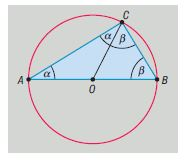
\includegraphics[width=0.4\linewidth]{Thalész.JPG}
			\caption{}
			\label{fig:thalesz}
		\end{figure}
		\begin{equation*}
			OA=OC=r\implies OAC \text{ háromszög egyenlő szárú} \implies OAC\angle=OCA\angle=\alpha
		\end{equation*}
		\begin{equation*}
		CA=OB=r\implies OBC \text{ háromszög egyenlő szárú}\implies OBC\angle=BCO\angle=\beta
		\end{equation*}
	\end{proof}
	\begin{theorem}[Thalész-tétel megfordítása]
		Ha egy háromszög derékszögű, akkor köré írható körének középpontja az átfogó felezőpontja.
	\end{theorem}
	\begin{theorem}[Magasságtétel]
		Derékszögű háromszögben az átfogóhoz tartozó magasság hossza mértani közepe azon két szakasz hosszának, amelyekre a magasság az átfogót osztja.
	\end{theorem}
	\begin{theorem}[Befogótétel]
		Derékszögű háromszög befogójának hossza mértani közepe az átfogó és a befogó
		átfogóra eső merőleges vetülete hosszának.
	\end{theorem}
	\begin{theorem}
		Derékszögű háromszög beírt körének sugara:
		\begin{equation*}
			r=\frac{a+b-c}{2}
		\end{equation*}
	\end{theorem}
\section{Hegyesszögek szögfüggvényeinek definíciója}
	Két derékszögű háromszög hasonló, ha 1 hegyesszögük megegyezik. Emiatt oldalainak arányát egyik hegyesszöge egyértelműen meghatározza. Erre a függvényszerű kapcsolatra vezetjük be a szögfüggvényeket.
	\begin{definition}
		Az $\alpha$ hegyesszöget tartalmazó tetszőleges derékszögű háromszögben:
		\begin{itemize}
			\item sin$\alpha$=$\frac{\alpha\text{-val szembeni befogó hossza}}{\text{Átfogó hossza}}$
			\item cos$\alpha$=$\frac{\alpha\text{ melletti befogó hossza}}{\text{Átfogó hossza}}$
			\item tg$\alpha$=$\frac{\alpha\text{-val szembeni befogó hossza}}{\alpha\text{ melletti befogó hossza}}$
			\item ctg$\alpha$=$\frac{\alpha\text{ melletti befogó hossza}}{\alpha\text{-val szembeni befogó hossza}}$
		\end{itemize}
		\begin{figure}[H]
			\centering
			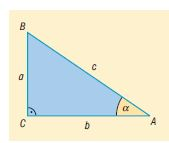
\includegraphics[width=0.4\linewidth]{Derékszög}
		\end{figure}
		\begin{equation*}
			\sin\alpha=\frac{a}{c},\ \cos\alpha=\frac{b}{c},\ \text{tg}\alpha=\frac{a}{b},\ \text{ctg}\alpha=\frac{b}{a}
		\end{equation*}
	\end{definition}
\section{Összefüggések a hegyesszögek szögfüggvényei között}
	\begin{align*}
		\text{tg}\alpha&=\frac{\sin\alpha}{\cos\alpha},\ \text{ctg}\alpha=\frac{\cos\alpha}{\sin\alpha},\ \text{tg}\alpha=\frac{1}{\text{ctg}\alpha}\\
		\sin\alpha&=\cos(90\degree-\alpha),\ \cos\alpha=\sin(90\degree-\alpha)\\
		\text{tg}\alpha&=\text{ctg}(90\degree-\alpha),\ \text{ctg}\alpha=\text{tg}(90\degree-\alpha)\\
		\sin^2\alpha+\cos^2\alpha&=1
	\end{align*}
	\begin{table}[H]
		\centering
		\begin{tabular}{|c||c|c|c|c|}
			\hline
			&sin&cos&tg&ctg\\\hline\hline
			30\degree&$\frac{1}{2}$&$\frac{\sqrt{3}}{2}$&$\frac{\sqrt{3}}{3}$&$\sqrt{3}$\\\hline
			45\degree&$\frac{\sqrt{2}}{2}$&$\frac{\sqrt{2}}{2}$&1&1\\\hline
			60\degree&$\frac{\sqrt{3}}{2}$&$\frac{1}{2}$&$\sqrt{3}$&$\frac{\sqrt{3}}{3}$\\\hline
		\end{tabular}
		\caption{Nevezetes szögek szögfüggvényei}
	\end{table}
\section{Szögfüggvények általánosítása}
	\begin{definition}
		A koordináta-rendszerben az $\underline{i}(1;0)$ bázisvektor origó körüli $\alpha$ szöggel való elforgatásával keletkező $\underline{e}$ egységvektor első koordinátája az $\alpha$ szög koszinusza, második koordinátája az $\alpha$ szög szinusza.
	\end{definition}
	\begin{definition}
		A $\frac{\sin\alpha}{\cos\alpha}$ hányadost, ha $\cos\alpha\ne0$, vagyis ha $\alpha\ne\frac{\pi}{2}+k\pi(k\in\mathbb{Z})$, az $\alpha$ szög tangensének nevezzük.
	\end{definition}
	A koordináta-rendszerben az $\underline{i}$ vektortól $\alpha$ szöggel elforgatott $\underline{e}$ egységvektor egyenese által az origó középpontú, egységsugarú kör $(1;0)$ pontjában húzott érintőből kimetszett pont 2. koordinátája az $\alpha$ szög tangense.
	\begin{definition}
		A $\frac{\cos\alpha}{\sin\alpha}$ hányadost, ha $\cos\alpha\ne0$, vagyis ha $\alpha\ne k\pi(k\in\mathbb{Z})$, az $\alpha$ szög kotangensének nevezzük.
	\end{definition}
	A koordináta-rendszerben az $\underline{i}$ vektortól $\alpha$ szöggel elforgatott $\underline{e}$ egységvektor egyenese által az origó középpontú, egységsugarú kör $(0;1)$ pontjában húzott érintőből kimetszett pont 1. koordinátája az $\alpha$ szög kotangense.
\section{Kapcsolat egy szög szögfüggvényei között}
	\begin{align*}
		\text{ctg}\alpha&=\frac{1}{\text{tg}\alpha}, \text{ ha }\alpha\ne k\frac{\pi}{2}\ (k\in\mathbb{Z})\\
		\text{tg}\alpha&=\frac{1}{\text{ctg}\alpha}, \text{ ha }\alpha\ne k\frac{\pi}{2}\ (k\in\mathbb{Z})\\
		\implies \text{tg}\alpha*\text{ctg}\alpha&=1\ (\alpha\ne k\frac{\pi}{2},\ k\in\mathbb{Z})\\
		\sin^2\alpha+\cos^2\alpha&=1\ \forall\alpha\in\mathbb{R}
	\end{align*}
\section{Alkalmazások}
	\begin{outline}
		\1 Pitagorasz-tétel
			\2 Koordinátageometria: két pont távolsága, vektor hossza
		\1 Forgásszögek szögfüggvényei:
			\2 Rezgőmozgás kitérés-idő, sebesség-idő, gyorsulás-idő függvénye
			\begin{align*}
				x(t)&=A*\sin(\omega t+\varphi_0)\\
				v(t)&=A\omega*\cos(\omega t+\varphi_0)\\
				a(t)&=-A\omega^2*\sin(\omega t+\varphi_0)\\
			\end{align*}
	\end{outline}
\section{Matematikatörténet}
	\begin{outline}
		\1 Pitagorasz (Kr. e. VI. század)
			\2 Tételét babilóniaiak is ismerték
			\2 Hozzá fűződik, mert rájött egy új bizonyítására
		\1 Leonhard Euler (XVIII. század)
			\2 Végtelen sorok
			\begin{align*}
				\sin(x)&=x-\frac{x^3}{3!}+\frac{x^5}{5!}-\dots=\sum_{n=0}^{\infty} \left(\frac{(-1)^n*x^{2n-1}}{(2n-1)!}\right)\\
				\cos(x)&=1-\frac{x^2}{2!}+\frac{x^4}{4!}-\dots=\sum_{n=0}^{\infty} \left(\frac{(-1)^n*x^{2n}}{(2n)!}\right)\\
			\end{align*}
			\2 Euler-képlet: $e^{ix}=\cos x+i\sin x$
	\end{outline}
\chapter{Háromszögek nevezetes vonalai, pontjai és körei}
\section{Oldalfelező merőlegesek, a háromszög köré írt kör középpontja}
	\begin{definition}
		A síkon egy szakasz felezőmerőlegese az az egyenes, amely a szakasz felezőpontjára
		illeszkedik és merőleges a szakaszra.
	\end{definition}
	\begin{theorem}
		A szakasz felezőmerőlegese a szakasz két végpontjától egyenlő távol lévő pontok halmaza.
	\end{theorem}
	\begin{theorem}
		A háromszög három oldalfelező merőlegese egy pontban metszi egymást. Ez a pont a háromszög
		köré írt kör középpontja.
	\end{theorem}
\section{Szögfelezők, háromszögbe, illetve háromszöghöz írt kör középpontja}
	\begin{definition}
		Egy konvex szög szögfelezője a szög csúcsából kiinduló, a szögtartományban haladó
		azon félegyenes, amely a szöget két egyenlő nagyságú szögre bontja.
	\end{definition}
	\begin{theorem}
		Egy konvex szögtartományban a száraktól egyenlő távolságra lévő pontok halmaza a szögfelező.
	\end{theorem}
	\begin{theorem}
		A háromszög három belső szögfelezője egy pontban metszi egymást. Ez a pont a háromszögbe
		írt kör középpontja.
	\end{theorem}
	\begin{theorem}
		A háromszög egy belső, és a másik két csúcshoz tartozó külső szögfelezője egy pontban
		metszi egymást, ez a pont a háromszög hozzáírt körének középpontja. A háromszögnek 3
		hozzáírt köre van.
	\end{theorem}
	\begin{theorem}
		A háromszög ugyanazon szögének külső és belső szögfelezője merőleges egymásra.
	\end{theorem}
\section{Magasságvonalak, a háromszög magasságpontja}
	\begin{definition}
		A háromszög magassága az egyik csúcsból a szemközti oldal egyenesére bocsátott merőleges szakasz. A háromszög magasságának egyenese a háromszög magasságvonala.
	\end{definition}
	\begin{theorem}
		A háromszög magasságvonalai egy pontban metszik egymást. Ez a pont a háromszög magasságpontja.
	\end{theorem}
	\begin{proof}
		\begin{figure}[H]
			\centering
			\includegraphics[width=0.6\linewidth]{Magasság}
		\end{figure}
		Húzzunk az ABC háromszög mindhárom csúcsán keresztül párhuzamos egyenest a szemközti oldallal, ez az A'B'C' háromszög.\\
		$\left(m_c\perp AB\right)\wedge\left(A'B'\perp AB\right)\implies m_c\perp A'B'$. $\left(AB\|A'B'\right)\wedge\left(BC\|B'C'\right)\\
		\implies$ ABCB' paralelogramma$\implies CB'=AB$. Hasonlóan ABA'C paralelogramma $\implies A'C=AB$, ezekből következik, hogy $B'C=CA'\implies C$ felezőpontja\\
		$A'B'$-nek$\implies m_c$ oldalfelező merőlegese $A'B'$-nek. 
		
		Hasonlóan belátható, hogy $m_a$ és $m_b$ is az $A'B'C'$ háromszög oldalfelező merőlegesei. Az oldalfelező merőlegesekre vonatkozó tétel alapján tudjuk, hogy ezek egy pontban metszik
		egymást, tehát beláttuk, hogy az $ABC$ háromszög magasságvonalai is egy pontban metszik
		egymást.
	\end{proof}
	A magasságpont hegyesszögű háromszög esetén a háromszög belsejében, derékszögű háromszögnél
	a derékszögű csúcsban, tompaszögű háromszögnél a háromszögön kívül helyezkedik el.
\section{Súlyvonalak, a háromszög súlypontja}
	\begin{definition}
		A háromszög csúcsát a szemközti oldal felezőpontjával összekötő szakasz a háromszög
		súlyvonala.
	\end{definition}
	\begin{theorem}
		A háromszög súlyvonalai egy pontban metszik egymást, ezt a pontot a háromszög súlypontjának
		nevezzük. A súlypont harmadolja a súlyvonalakat úgy, hogy a csúcs felé eső szakasz és az oldal felé eső szakasz aránya $2:1$.
	\end{theorem}
\section{Középvonalak}
	\begin{definition}
		A háromszög két oldalfelező pontját összekötő szakaszt a háromszög középvonalának
		nevezzük. Minden háromszögnek 3 középvonala van.
	\end{definition}
	\begin{theorem}
		A háromszög középvonala párhuzamos a felezőpontokat nem tartalmazó oldallal, és fele
		olyan hosszú.
	\end{theorem}
\pagebreak
\section{Euler-egyenes, Feuerbach-kör}
	\begin{theorem}[Euler-egyenes]
		A háromszög magasságpontja, súlypontja és a körülírt kör középpontja egy egyenesen van. A súlypont a másik kettő távolságát harmadolja és a körülírt kör középpontjához van közelebb.
	\end{theorem}
	\begin{figure}[H]
		\centering
		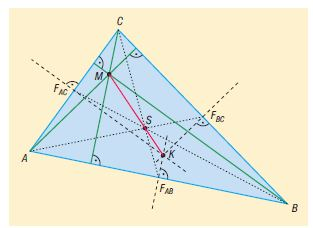
\includegraphics[width=0.5\linewidth]{Euler}
	\end{figure}
	\begin{theorem}[Feuerbach-kör]
		Egy háromszög oldalainak felezőpontjai, magasságainak talppontjai és a magasságpontot
		a csúcsokkal összekötő szakaszok felezőpontjai egy körön vannak. Feuerbach kör középpontja (O) felezi a magasságpontot (M) és a köré írható kör középpontját (K) összekötő szakaszt, sugara a háromszög köré írható kör sugarának a fele. Azaz a Feuerbach-kör a körülírható kör M pontra vonatkozó $\lambda=\frac{1}{2}$ arányú középpontos hasonlóság képe.
	\end{theorem}
	\begin{figure}[H]
		\centering
		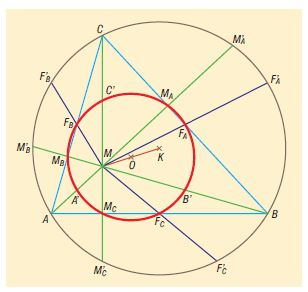
\includegraphics[width=0.5\linewidth]{Feuerbach}
	\end{figure}
	\begin{theorem}
		Egy háromszög Feuerbach-köre érinti a háromszög beírt körét, és hozzáírt köreit.
	\end{theorem}
\section{Alkalmazások}
	\begin{outline}
		\1 Súlyvonal, súlypont: ott alátámasztva egyensúlyban van
		\1 Területszámítás a körök sugarainak felhasználásával: $R=\frac{abc}{4T},\ r=\frac{T}{s}$, ahol $s=\frac{K}{2}$
	\end{outline}
\section{Matematikatörténet}
	\begin{outline}
		\1 Euklidesz (Kr. e. 300 körül)
			\2 Elemek című műve: geometriai axiómák, belőlük bizonyított tételek, szerkesztési módok
			\2 Szerepelnek olyan tételek is, melyek nem következnek az axiómákból
			\2 Pl.:  $ABC$ háromszög, $l$ egyenes $P$-n keresztül, $ABC$ egyik oldalán. Létezik $Q$ a háromszög másik oldalán, $l$ átmegy $Q$-n.
				\3 Pasch fedezte fel XIX. században
		\1 Hilbert (XIX. század)
			\2 20 axióma geometriára
		\1 Euler (XVIII. század) 
			\2 Háromszög nevezetes vonalait, pontjait is vizsgálta. Ő is ismerte a Feuerbach-kört.
		\1 Feuerbach (XIX. század)
			\2 Bizonyította, hogy a Feuerbach-kör érinti a beírt, és hozzáírt köröket
	\end{outline}
\chapter{Összefüggések általános háromszögben}
\section{Háromszögek csoportosítása}
	\begin{definition}
		Háromszög az a zárt szögvonal, amelyeknek 3 oldala és 3 csúcsa van.
	\end{definition}
	\begin{definition}
		Egy háromszög hegyesszögű, ha minden szöge hegyesszög.
	\end{definition}
	\begin{definition}
		Egy háromszög derékszögű, ha van egy 90\degree-os szöge.
	\end{definition}
	\begin{definition}
		Egy háromszög tompaszögű, ha van egy tompaszöge.
	\end{definition}
	\begin{definition}
		Egy háromszög szabályos, ha három oldala egyenlő hosszú.
	\end{definition}
	\begin{definition}
		Egy háromszög egyenlő szárú, ha van két egyenlő oldala.
	\end{definition}
	\begin{figure}[H]
		\centering
		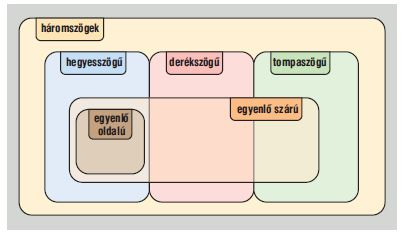
\includegraphics[width=0.6\linewidth]{Csoport}
	\end{figure}
\section{Összefüggések a háromszög oldalai között}
	\begin{theorem}[Háromszög-egyenlőtlenség]
		A háromszög bármely két oldalának összege nagyobb a harmadiknál:
		\begin{equation*}
			a+b>c,\ a+c>b,\ b+c>a
		\end{equation*}
	\end{theorem}
	\begin{theorem}
		Egy háromszögben bármely két oldal különbségének abszolút értéke kisebb a harmadiknál:
		\begin{equation*}
			|a-c|<b,\ |a-b|<c,\ |b-c|<a
		\end{equation*}
	\end{theorem}
	\begin{theorem}[Pitagorasz-tétel]
		Bármely derékszögű háromszögben a két befogó négyzetének összege egyenlő az átfogó négyzetével.
	\end{theorem}
\section{Összefüggések a háromszög szögei között}
	\begin{theorem}
		A háromszög belső szögeinek összege: 180\degree
	\end{theorem}
	\begin{theorem}
		A háromszög külső szögeinek összege: 360\degree
	\end{theorem}
	\begin{theorem}
		A háromszög egy külső szöge egyenlő a nem mellette fekvő két belső szög összegével.
	\end{theorem}
\section{Összefüggések a háromszög oldalai és szögei között}
	\begin{theorem}
		Egy háromszögben egyenlő hosszúságú oldalakkal szemben egyenlő nagyságú szögek vannak,
		és egyenlő nagyságú szögekkel szemben egyenlő hosszúságú oldalak vannak.
	\end{theorem}
	\begin{theorem}
		Bármely háromszögben két oldal közül a hosszabbikkal szemben nagyobb belső szög van, illetve két szög közül a nagyobbikkal szemben hosszabb oldal van.
	\end{theorem}
\pagebreak
	\begin{definition}
		Derékszögű háromszögben bevezetjük a szögfüggvények fogalmát a hasonló háromszögek
		tulajdonságait kihasználva:
		\begin{itemize}
			\item sin$\alpha$=$\frac{\alpha\text{-val szembeni befogó hossza}}{\text{Átfogó hossza}}$
			\item cos$\alpha$=$\frac{\alpha\text{ melletti befogó hossza}}{\text{Átfogó hossza}}$
			\item tg$\alpha$=$\frac{\alpha\text{-val szembeni befogó hossza}}{\alpha\text{ melletti befogó hossza}}$
			\item ctg$\alpha$=$\frac{\alpha\text{ melletti befogó hossza}}{\alpha\text{-val szembeni befogó hossza}}$
		\end{itemize}
		\begin{figure}[H]
			\centering
			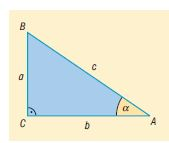
\includegraphics[width=0.4\linewidth]{Derékszög}
		\end{figure}
		\begin{equation*}
		\sin\alpha=\frac{a}{c},\ \cos\alpha=\frac{b}{c},\ \text{tg}\alpha=\frac{a}{b},\ \text{ctg}\alpha=\frac{b}{a}
		\end{equation*}
	\end{definition}
	\begin{theorem}[Szinusztétel]
		Egy háromszögben a három oldal áranya megegyezik a velük szemben lévő oldalak szinuszának arányával:
		\begin{equation*}
			a:b:c=\sin\alpha:\sin\beta:\sin\gamma
		\end{equation*}
	\end{theorem}
	\begin{outline}
		\1 Alkalmazása:
			\2 1 oldal, 2 szög -> bármely oldal
			\2 2 oldal, nem közbezárt szög:
				\3 Nagyobbik oldallal szembeni szög -> kisebbikkel szembeni szög
					\4 Háromszög egyértelműen meghatározott
				\3 Rövidebbel szembeni szög -> nagyobbikkal szembeni szög
					\4 Ha szinusz kisebb 1-nél: két megoldás. Háromszög nem egyértelműen meghatározott.
					\4 Ha szinusz egyenlő 1-el: egy megoldás 90\degree. A háromszög derékszögű
					\4 Ha szinusz nagyobb 1-nél: nincs ilyen háromszög
	\end{outline}
	\begin{theorem}[Koszinusztétel]
		Egy háromszög egy oldalának négyzete egyenlő a másik két oldal négyzetösszegéből kivonva a két oldal hosszának és a közbezárt szög koszinuszának kétszeres szorzatát:
		\begin{equation*}
			c^2=a^2+b^2-2ab\cos\gamma
		\end{equation*}
	\end{theorem}
	\begin{proof}
		Vezessük be a következő vektorokat:
		\begin{equation*}
			\overrightarrow{CB}=\underline{a},\ \overrightarrow{CA}=\underline{b},\ \overrightarrow{BA}=\underline{c}
		\end{equation*}
		Legyen: $|\underline{a}|=a,\ |\underline{b}|=b,\ |\underline{c}|=c$
		\begin{figure}[H]
			\centering
			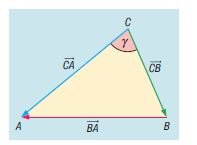
\includegraphics[width=0.5\linewidth]{Cos}
		\end{figure}
		Ekkor $\underline{c}=\vec{a}-\vec{b}$. Az egyenlet két oldalát négyzetre emelve:
		\begin{align*}
			\vec{c}^2&=(\vec{a}-\vec{b})^2\\
			\vec{c}^2&=\vec{a}^2-2\vec{a}\vec{b}+\vec{b}^2\\
			c^2&=a^2+b^2-2ab\cos\gamma
		\end{align*}
	\end{proof}
	Következmények:
	\begin{itemize}
		\item Ha a háromszög derékszögű, akkor $c^2=a^2+b^2$, ami a Pitagorasz-tétel.
		\item Ha a háromszög hegyesszögű, akkor bármely két oldalának négyzetösszege nagyobb a harmadik oldal négyzeténél.
		\item Ha a háromszög tompaszögű, akkor a két rövidebb oldal négyzetösszege kisebb a harmadik oldal négyzeténél.
	\end{itemize}
	\begin{outline}
		\1 Alkalmazás:
			\2 2 oldal, közbezárt szög -> szemközti oldal
			\2 3 oldal -> bármely szög
				\3 Legnagyobbat érdemes kiszámolni, mert egyértelmű megoldást ad
	\end{outline}
\section{Alkalmazások}
	\begin{outline}
		\1 Háromszög ismeretlen adatainak kiszámítása
		\1 Földmérésben, térképészetben, csillagászatban mért adatokból távolságok és szögek kiszámolása
		\1 Modern helymeghatározás: GPS
	\end{outline}
\section{Matematikatörténet}
	\begin{outline}
		\1 Abu Nasr (1000 körül)
			\2 Szinusztétel
		\1 Thalész (Kr. e. VI. század)
			\2 Belső szögek összege 180\degree
			\2 Egyenlő hosszú oldalakkal szemben egyenlő szögek
		\1 Euklidesz (Kr. e. 300 körül)
			\2 Elemek című műve: geometriai axiómák, belőlük bizonyított tételek, szerkesztési módok
			\2 Szerepelnek olyan tételek is, melyek nem következnek az axiómákból
			\2 Pl.:  $ABC$ háromszög, $l$ egyenes $P$-n keresztül, $ABC$ egyik oldalán. Létezik $Q$ a háromszög másik oldalán, $l$ átmegy $Q$-n.
				\3 Pasch fedezte fel XIX. században
		\1 Hilbert (XIX. század)
			\2 20 axióma geometriára
	\end{outline}
\chapter{Egybevágóság és hasonlóság}
\section{Transzformációk}
	\begin{definition}
		Geometriai transzformációk azok a függvények, amelyek egy ponthalmazt ponthalmazra képeznek le.
	\end{definition}
	\begin{definition}[Távolságtartó leképezés]
		Bármely két pont távolsága egyenlő képeik távolságával.
	\end{definition}
	\begin{definition}
		A geometriai transzformációk közül a távolságtartó transzformációkat egybevágósági
		transzformációknak nevezzük.
	\end{definition}
	Síkbeli egybevágósági transzformációk: tengelyes tükrözés, pontra vonatkozó (középpontos)
	tükrözés, pont körüli elforgatás, eltolás.
	\begin{definition}[Tengelyes tükrözés]
		Adott a sík egy $t$ egyenese, ez a tengelyes tükrözés tengelye. A $t$ tengelyre vonatkozó tengelyes tükrözés a sík tetszőleges $t$-re nem illeszkedő $P$ pontjához azt a $P'$ pontot rendeli, amelyre fennáll, hogy a $PP'$ szakasz felezőmerőlegese a t tengely. A $t$ egyenes képe önmaga.
	\end{definition}
	\begin{figure}[H]
		\centering
		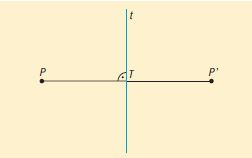
\includegraphics[width=0.3\linewidth]{Tengely}
	\end{figure}
	\begin{definition}[Középpontos tükrözés]
		Adott a sík egy $O$ pontja, a középpontos tükrözés középpontja. Az $O$ pontra vonatkozó középpontos tükrözés a sík egy tetszőleges $O$-tól különböző $P$ pontjához azt a $P'$ pontot rendeli, amelyre az $O$ pont a $PP'$ szakasz felezőpontja Az $O$ pont képe önmaga.
	\end{definition}
	\begin{figure}[H]
		\centering
		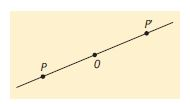
\includegraphics[width=0.3\linewidth]{KPont}
	\end{figure}
	\begin{definition}[Pont körüli forgatás]
		Adott a sík egy $O$ pontja és egy $\alpha$ irányított szög. Az $O$ pont körüli $\alpha$ szögű a sík egy tetszőleges $O$-tól különböző $P$ pontjához azt a $P'$ pontot rendeli, amelyre teljesül, hogy $POP'\angle$ irány és nagyság szerint megegyezik $\alpha$-val és $OP = OP'$. Az $O$ pont képe önmaga.
	\end{definition}
	\begin{figure}[H]
		\centering
		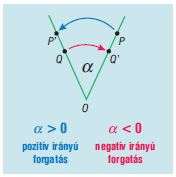
\includegraphics[width=0.3\linewidth]{Forg}
	\end{figure}
	\begin{definition}[Eltolás]
		Adott egy $\vec{v}$ vektor. A $\vec{v}$ vektorral való eltolás a sík tetszőleges $P$ pontjához azt a $P'$ pontot rendeli, amelyre $\overrightarrow{PP'}=\vec{v}$.
	\end{definition}
	\begin{figure}[H]
		\centering
		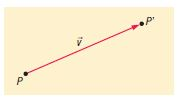
\includegraphics[width=0.3\linewidth]{Elt}
	\end{figure}
\section{Alakzatok egybevágósága}
	\begin{definition}
		Két alakzat egybevágó, ha van olyan egybevágósági transzformáció, amely az egyik alakzatot a másikba viszi. Jele: $A\cong B$.
	\end{definition}
	\begin{theorem}
		Két háromszög akkor, és csak akkor egybevágó, ha:
		\begin{itemize}
			\item Megfelelő oldalaik hossza páronként egyenlő
			\item 2-2 oldaluk hossza páronként egyenlő, és az ezek által közbezárt szögek nagysága egyenlő
			\item 2-2 oldaluk hossza páronként egyenlő és e 2-2 oldal közül a hosszabbikkal szemközti szögük nagysága egyenlő
			\item 1-1 oldaluk hossza páronként egyenlő és két-két szögük páronként egyenlő
		\end{itemize}
	\end{theorem}
	\begin{theorem}
		Két sokszög akkor és csak akkor egybevágó, ha a következő feltételek egyike teljesül:
		\begin{itemize}
			\item Megfelelő oldalaik hossza és a megfelelő átlóik hossza páronként egyenlő
			\item Megfelelő oldalaik hossza páronként egyenlő és megfelelő szögeik páronként egyenlők
		\end{itemize}
	\end{theorem}
\section{Hasonlósági transzformáció: középpontos hasonlóság}
	\begin{definition}[Középpontos hasonlósági transzformáció]
		Adott egy $O$ pont, a transzformáció középpontja, és egy $\lambda$ 0-tól különböző valós szám, a hasonlóság aránya. A transzformáció a sík tetszőleges $P$ pontjához azt a $P'$ pontot rendeli, amely az $OP$ egyenes azon pontja, amelyre $OP'=|\lambda|*OP$, és ha $\lambda>0$, akkor $P'\in\ray{OP}$, ha $\lambda<0$, akkor $P'\notin \ray{OP}$ 
	\end{definition}
	Ha $|\lambda|>1$, akkor középpontos nagyításról, ha $|\lambda|<1$, akkor kicsinyítésről beszélünk, ha $|\lambda|=1$, akkor a transzformáció egybevágóság.
	\begin{definition}
		Véges sok középpontos hasonlósági transzformáció és véges sok egybevágósági transzformáció
		egymás utáni végrehajtásával kapott transzformációkat hasonlósági transzformációnak nevezzük.
	\end{definition}
\section{Alakzatok hasonlósága}
	\begin{definition}
		Két alakzat hasonló, ha van olyan hasonlósági transzformáció, amely az egyik alakzatot a másikba viszi. Jele: $A\sim B$.
	\end{definition}
	\begin{theorem}
		Két háromszög akkor és csak akkor hasonló, ha:
		\begin{itemize}
			\item Megfelelő oldalaik hossza páronként egyenlő
			\item 2-2 oldalhosszuk aránya, és az ezek által közbezárt szögek nagysága egyenlő
			\item 2-2 oldalhosszuk aránya egyenlő, és e 2-2 oldal közül a hosszabbikkal szemközti szögük nagysága egyenlő
			\item 2-2 szögük páronként egyenlő
		\end{itemize}
	\end{theorem}
	\begin{theorem}
		Két sokszög akkor és csak akkor hasonló, ha megfelelő oldalhosszaik aránya és megfelelő szögeik nagysága páronként egyenlő nagyságú.
	\end{theorem}
\section{Transzformációk főbb tulajdonságai}
	\begin{figure}[H]
		\centering
		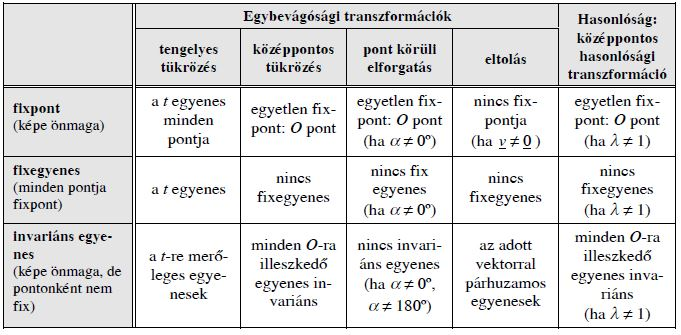
\includegraphics[width=\linewidth]{Hasonl}
	\end{figure}
\section{Hasonlóság alkalmazása háromszögekre vonatkozó tételekben}
	\begin{theorem}
		A háromszög középvonala párhuzamos a felezőpontokat nem tartalmazó oldalakkal, és fele olyan hosszú, mint a nem felezett oldal.
	\end{theorem}
	\begin{theorem}
		A háromszög súlyvonalai egy pontban metszik egymást. Ez a pont mindhárom súlyvonalnak a csúcstól távolabbi harmadolópontja.
	\end{theorem}
	\begin{theorem}[Szögfelezőtétel]
		Egy háromszög belső szögfelezője a szemközti oldalt a szomszédos oldalak
		arányában osztja.
	\end{theorem}
	\begin{proof}
		Az $ABC$ háromszög $A$ csúcsából induló belső szögfelező $BC$ oldalt az $S$ pontban
		metszi. A $BA$ szakaszt hosszabbítsuk meg $A$-n túl és legyen $AD = b$. Ekkor $AD = AC = b$, ebből következik, hogy az $ACD$ háromszög egyenlő szárú, a $C$-nél és a $D$-nél levő belső szögek egyenlők, az $A$-nál levő külső szög $\alpha$.
		\begin{figure}[H]
			\centering
			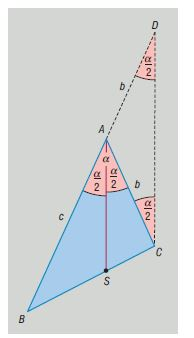
\includegraphics[width=0.3\linewidth]{SZFT}
		\end{figure}
		
		$CAD\angle=180\degree-\alpha\implies ACD\angle=ADC\angle=\frac{\alpha}{2}$. $BAS\angle=ADC\angle=\frac{\alpha}{2}\implies AS\|CD$. $CBA\angle$-ra alkalmazva a párhuzamos szelők tételét:
		\begin{equation*}
			\frac{CS}{SB}=\frac{DA}{AB}=\frac{AC}{AB}
		\end{equation*}
	\end{proof}
	\begin{theorem}[Magasságtétel]
		Derékszögű háromszögben az átfogóhoz tartozó magasság hossza mértani közepe azon két szakasz hosszának, amelyekre a magasság az átfogót osztja.
	\end{theorem}
	\begin{theorem}[Befogótétel]
		Derékszögű háromszög befogójának hossza mértani közepe az átfogó és a befogó átfogóra eső merőleges vetülete hosszának.
	\end{theorem}
\section{Alkalmazások}
	\begin{outline}
		\1 Hegyesszögek szögfüggvényének értelmezése: derékszögű háromszögek hasonlósága
		\1 Szakasz egyenlő részekre osztása: párhuzamos szelők tétele
	\end{outline}
\section{Matematikatörténet}
	\begin{outline}
		\1 Euklidesz (Kr. e. 300 körül)
			\2 Elemek című műve: geometriai axiómák, belőlük bizonyított tételek, szerkesztési módok
			\2 Szerepelnek olyan tételek is, melyek nem következnek az axiómákból
			\2 Pl.:  $ABC$ háromszög, $l$ egyenes $P$-n keresztül, $ABC$ egyik oldalán. Létezik $Q$ a háromszög másik oldalán, $l$ átmegy $Q$-n.
				\3 Pasch fedezte fel XIX. században
		\1 Hilbert (XIX. század)
			\2 20 axióma geometriára 
	\end{outline}
\chapter{Kör és részei}
\section{Kör és részei}
	\begin{definition}
		Azoknak a pontoknak a halmaza a síkon amelyeknek a sík egy adott $O$ pontjától adott
		$r$ távolságra vannak $O$ középpontú, $r$ sugarú körnek nevezzük.
	\end{definition}
	\begin{definition}
		Azoknak a pontoknak a halmaza a síkon amelyeknek a sík egy adott $O$ pontjától adott
		$r$ távolságnál nem nagyobb/kisebb távolságra vannak $O$ középpontú, $r$ sugarú zárt/nyílt körlapnak nevezzük.
	\end{definition}
	\begin{definition}
		A körvonal két különböző pontját összekötő szakaszt húrnak nevezzük.
	\end{definition}
	\begin{definition}
		húr egyenesét szelőnek, a középponton áthaladó húrt átmérőnek nevezzük. Az átmérő
		a kör leghosszabb húrja, hossza: $2r$.
	\end{definition}
	\begin{theorem}
		A kör:
		\begin{itemize}
			\item középpontján áthaladó tetszőleges egyenesre nézve tengelyesen szimmetrikus
			\item középpontjára nézve középpontosan szimmetrikus
			\item középpontja körüli forgatásra forgásszimmetrikus
		\end{itemize}
	\end{theorem}
	\begin{definition}
		A körlapnak két sugár közé eső darabja a körcikk.
	\end{definition}
	\begin{definition}
		Egy szelő által a körlapból lemetszett rész a körszelet.
	\end{definition}
	\begin{definition}
		Két kör koncentrikus, ha középpontjaik egybeesnek.
	\end{definition}
	\begin{definition}
		Két koncentrikus körvonal közé eső rész a körgyűrű.
	\end{definition}
	\begin{definition}
		Ha egy szög csúcsa a kör középpontja akkor a szöget középponti szögnek nevezzük.
	\end{definition}
	\begin{theorem}
		Egy adott körben két középponti szöghöz tartozó ívek hosszának aránya, valamint a körcikkek
		területének aránya megegyezik a középponti szögek arányával.
		\begin{equation*}
			\frac{\alpha}{\beta}=\frac{i_\alpha}{i_\beta}=\frac{T_\alpha}{T_\beta}
		\end{equation*}
		\begin{figure}[H]
			\centering
			\includegraphics[width=0.3\linewidth]{Kör1}
		\end{figure}
	\end{theorem}
	\begin{theorem}
		Egy körben $\alpha$ középponti szögű körcikkhez tartozó ív hossza:
		\begin{equation*}
			i_\alpha=2r\pi*\frac{\alpha\degree}{360\degree}=r*\wideparen{\alpha}
		\end{equation*}
		A terület:
		\begin{equation*}
			T_\alpha=r^2\pi*\frac{\alpha\degree}{360\degree}=\frac{r^2*\wideparen{\alpha}}{2}=\frac{r*i_\alpha}{2}
		\end{equation*}
	\end{theorem}
	\begin{theorem}
		$R$ és $r$ határolta körgyűrű területe:
		\begin{equation*}
			T=R^2\pi-r^2\pi
		\end{equation*}
	\end{theorem}
	\begin{theorem}
		Körszelet területe:
		\begin{equation*}
			T=\frac{r^2*\wideparen{\alpha}}{2}-\frac{r^2\sin\alpha}{2}=\frac{r^2}{2}\left(\wideparen{\alpha}-\sin\alpha\right)
		\end{equation*}
	\end{theorem}
\section{Középponti és kerületi szögek}
	\begin{definition}
		Ha egy szög csúcsa egy adott körvonal egy pontja, szárai a kör két húrja, akkor a szöget kerületi szögnek nevezzük.
	\end{definition}
	\begin{definition}
		Ha egy szög csúcsa egy adott körvonal egy pontja, egyik szára a kör húrja, másik szára a körvonal adott pontbeli érintője, akkor a szöget érintőszárú kerületi szögnek nevezzük.
	\end{definition}
	\begin{theorem}[Középponti és kerületi szögek tétele]
		Adott körben adott ívhez tartozó bármely kerületi szög nagysága fele az ugyanazon ívhez tartozó középponti szög nagyságának.
	\end{theorem}
	\begin{proof}
		4 eset van:
		\begin{outline}[enumerate]
			\1 Középponti és kerületi szög szára egy egyenesbe esik.
				\begin{figure}[H]
					\centering
					\includegraphics[width=0.4\linewidth]{1sz}
				\end{figure}
				\2 $BOC$ egyenlő szárú, azaz: $OB=OC=r\implies OCB\angle=CBO\angle=\alpha$.
				\2 $\beta$ $OBC$ külső szöge, egyenlő két nem mellette fekvő belső szög összegével: $\beta=2\alpha\implies\alpha=\frac{\beta}{2}$.
			\1 A középponti szög csúcsa a kerületi szög belsejébe esik
				\begin{figure}[H]
					\centering
					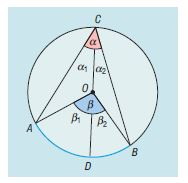
\includegraphics[width=0.4\linewidth]{2sz}
				\end{figure}
				\2 $BD$, $AD$ ívekhez tartozó szögek elhelyezkedése az 1. esetnek megfelelő, ezért: $\beta_1=2\alpha_1$, $\beta_2=2\alpha_2$.
				\2 $\implies \beta=\beta_1+\beta_2=2(\alpha_1+\alpha_2)\implies\alpha=\frac{\beta}{2}$
			\1 A középponti szög csúcsa a kerületi szög szögtartományán kívül esik
				\begin{figure}[H]
					\centering
					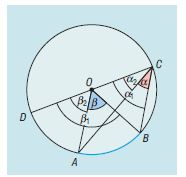
\includegraphics[width=0.4\linewidth]{3sz}
				\end{figure}
				\2 $\alpha=\alpha_1-\alpha_2,\ \beta=\beta_1-\beta_2$. Első eset miatt: $\alpha_1=\frac{\beta_1}{2},\ \alpha_2=\frac{\beta_2}{2}$
				\2 $\implies \alpha=\frac{\beta}{2}$
			\1 Érintőszárú a kerületi szög
				\begin{figure}[H]
					\centering
					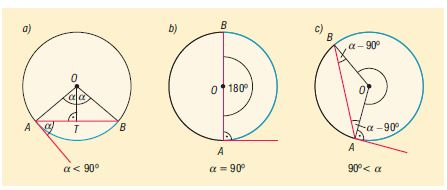
\includegraphics[width=0.8\linewidth]{4sz}
				\end{figure}
				\2 $\alpha<90\degree$
					\3 $BAO\angle=ABO\angle=90\degree-\alpha\implies AOB\angle=2\alpha=\beta$
					\3 $\implies \alpha=\frac{\beta}{2}$
				\2 $\alpha=90\degree\implies\beta=180\degree\implies \alpha=\frac{\beta}{2}$
				\2 $\alpha>90\degree$
					\3  $BAO\angle=ABO\angle=90\degree-\alpha\implies AOB\angle= 180\degree- 2(\alpha-90\degree)=360\degree-2\alpha$
					\3 $\implies\beta=2\alpha\implies\alpha=\frac{\beta}{2}$ 
		\end{outline}
	\end{proof}
	\begin{theorem}[Kerületi szögek tétele]
		Egyenlő sugarú körökben az azonos hosszúságú ívekhez tartozó kerületi szögek egyenlő nagyságúak.
	\end{theorem}
	\begin{theorem}[Thalész-tétele]
		Azon pontok halmaza síkon, amelyekből a sík egy AB szakasza derékszögben látszik, az AB átmérőjű körvonal, kivéve az A és a B pontokat.
	\end{theorem}
	\begin{definition}
		Tekintsünk egy $AB$ szakaszt és egy $P$ pontot. Legyen $APB\angle=\alpha$. Ekkor azt mondhatjuk, hogy a $P$ pontból az $AB$ szakasz $\alpha$ szög alatt látszik. Az $\alpha$ szöget látószögnek nevezzük.
	\end{definition}
	\begin{definition}
		Azon pontok halmaza amelyekből a sík egy $AB$ szakasza adott $\alpha\  (0\degree<\alpha<180\degree)$ szög alatt látszik, két, az $AB$ egyenesre szimmetrikusan elhelyezhető körív, melynek neve az $AB$ szakasz $\alpha$ szögű látóköríve. A szakasz két végpontja nem tartozik a ponthalmazba.
	\end{definition}
	\begin{figure}[H]
		\centering
		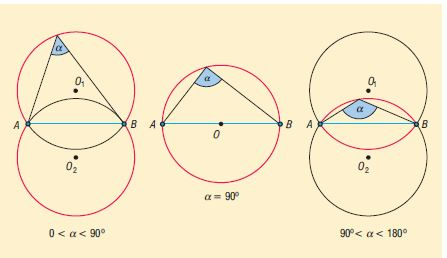
\includegraphics[width=0.7\linewidth]{Lato}
	\end{figure}
\section{Húrnégyszög}
	\begin{definition}
		Azokat a négyszögeket, amelyeknek van köré írható körük, húrnégyszögeknek nevezzük.
	\end{definition}
	\begin{theorem}[Húrnégyszög-tétel]
		Egy négyszög akkor és csak akkor húrnégyszög, ha szemközti szögeinek összege 180\degree.
	\end{theorem}
	\begin{theorem}
		Biztosan húrnégyszög a szimmetrikus trapéz (húrtrapéz), a téglalap, és a négyzet.
	\end{theorem}
	\begin{theorem}
		A paralelogramma akkor és csak akkor húrnégyszög, ha téglalap.
	\end{theorem}
	\begin{theorem}
		A húrnégyszög területe:
		\begin{equation*}
			T=\sqrt{(s-a)(s-b)(s-c)(s-d)}
		\end{equation*}
	\end{theorem}
\section{Érintőnégyszög}
	\begin{definition}
		Azokat a négyszögeket, amelyeknek van beírt körük, érintőnégyszögeknek nevezzük.
	\end{definition}
	\begin{theorem}[Érintőnégyszög-tétel]
		Egy konvex négyszög akkor és csak akkor érintőnégyszög, ha szemközti oldalainak összege egyenlő.
	\end{theorem}
	\begin{theorem}
		Biztosan érintőnégyszög a deltoid, a rombusz, és a négyzet
	\end{theorem}
	\begin{theorem}
		A paralelogramma akkor és csak akkor érintőnégyszög, ha rombusz.
	\end{theorem}
	\begin{theorem}
		Érintőnégyszög területe:
		\begin{equation*}
			T=\frac{K*r}{2}=s*r
		\end{equation*}
	\end{theorem}
\section{Alkalmazások}
	\begin{outline}
		\1 Körhöz húzott érintő és szelőszakaszok tétele: szakasz aranymetszésnek megfelelő felosztása
		\begin{figure}[H]
			\centering
			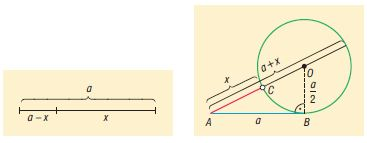
\includegraphics[width=.7\linewidth]{Arany}
		\end{figure}
		\1 Körrel kapcsolatos ismeretek: körmozgás, forgómozgás
	\end{outline}
\section{Matematikatörténet}
	\begin{outline}
		\1 Euklidesz (Kr. e. 300 körül)
			\2 Elemek című műve: geometriai axiómák, belőlük bizonyított tételek, szerkesztési módok
			\2 Szerepelnek olyan tételek is, melyek nem következnek az axiómákból
			\2 Pl.:  $ABC$ háromszög, $l$ egyenes $P$-n keresztül, $ABC$ egyik oldalán. Létezik $Q$ a háromszög másik oldalán, $l$ átmegy $Q$-n.
				\3 Pasch fedezte fel XIX. században
		\1 Hilbert (XIX. század)
			\2 20 axióma geometriára 
		\1 Hérón (Kr. e. I. század)
			\2 Hérón-képlet
		\1 Leonardo da Vinci (XV-XVI. század)
			\2 Számos festményében használta az aranymetszést
	\end{outline}
\chapter{Vektorok}
\section{Vektor}
	A vektor alapfogalom, nem definiáljuk, azonban szemléletesen lehet irányított szakasznak nevezni. Jele: $\overrightarrow{AB}=\vec{v}$, $A:$ kezdőpont $B:$ végpont
	\begin{definition}
		A vektor abszolút értéke a vektort meghatározó irányított szakasz hossza. Jele: $|\overrightarrow{AB}|$.
	\end{definition}
	\begin{definition}
		Az a vektor amelynek abszolút értéke 0, nullvektor. Jele: $\vec{0}$. Iránya tetszőleges.
	\end{definition}
	\begin{definition}
		Két vektor egyirányú, ha a két vektor párhuzamos, és azonos irányba mutat.
	\end{definition}
	\begin{definition}
		Két vektor ellentétes irányú, ha a két vektor párhuzamos, és ellentétes irányba mutat.
	\end{definition}
	\begin{definition}
		Két vektor egyenlő, ha egyirányúak és abszolút értékük egyenlő.
	\end{definition}
	\begin{definition}
		Két vektor egymás ellentettje, ha ellentétes irányúak és abszolút értékük egyenlő.
	\end{definition}
\section{Vektorműveletek}
	\begin{definition}
		Az $\vec{a}$ és $\vec{b}$ vektorok összege annak az eltolásnak a vektora, amellyel helyettesíthető az először $\vec{a}$ vektorral, majd a $\vec{b}$ vektorral történő eltolás. Jele: $\vec{a}+\vec{b}$.
	\end{definition}
	\begin{figure}[H]
		\centering
		\includegraphics[width=0.8\linewidth]{Összeg}
	\end{figure}
	\begin{outline}
		\1 Tulajdonságok
			\2 $\vec{a}+(-\vec{a})=\vec{0}$
			\2 Kommutatív: $\vec{a}+\vec{b}=\vec{b}+\vec{a}$
			\2 Asszociatív: $(\vec{a}+\vec{b})+\vec{c}=\vec{a}+(\vec{b}+\vec{c})$
	\end{outline}
	\begin{definition}
		Az $\vec{a}-\vec{b}$ különbségvektor az a vektor, amelyhez a $\vec{b}$ vektort adva az $\vec{a}$ vektort kapjuk. Jele: $\vec{a}-\vec{b}$
	\end{definition}
	\begin{figure}[H]
		\centering
		\includegraphics[width=0.4\linewidth]{Kül}
	\end{figure}
	$\vec{a}-\vec{b}$, és $\vec{b}-\vec{a}$ egymás ellentettjei.
	\begin{definition}
		Egy $\vec{a}$ vektor tetszőleges $\lambda$ valós számmal (skalár) vett szorzata olyan vektor, amely abszolút értéke $|\lambda|*|\vec{a}|$ és $\lambda>0$ esetén $\vec{a}$-val egyirányú, egyébként ellentétes irányú
	\end{definition}
	\begin{outline}
		\1 Tulajdonságok
			\2 Disztributív: 
			\begin{align*}
				\alpha*\vec{a}+\beta*\vec{a}&=(\alpha+\beta)*\vec{a}\\
				\alpha*\vec{a}+\alpha*\vec{b}&=\alpha*(\vec{a}+\vec{b})
			\end{align*}
			\2 Asszociatív: 
			\begin{equation*}
				\alpha*(\beta*\vec{a})=(\alpha*\beta)*\vec{a}
			\end{equation*}
	\end{outline}
\section{Vektorok felbontása}
	\begin{definition}
		Tetszőleges $\vec{a},\vec{b}$ vektorokkal és $\alpha,\beta$ valós számokkal képzett $\vec{v}=\alpha*\vec{a}+\beta*\vec{b}$ vektort az $\vec{a},\vec{b}$ vektorok lineáris kombinációjának nevezzük.
	\end{definition}
	\begin{theorem}
		Ha $\vec{a};\vec{b}\ne\vec{0}$ és $\vec{a}\|\vec{b}$, akkor pontosan egy olyan $\alpha\in\mathbb{R}$ létezik, hogy $\vec{b}=\alpha*\vec{a}$.
	\end{theorem}
	\begin{theorem}
		Ha $\vec{a};\vec{b}\ne\vec{0},\ \vec{a}\|\vec{b}$, akkor a velük egy síkban lévő minden $\vec{c}$ vektor egyértelműen előáll $\vec{a}$ és $\vec{b}$ vektorok lineáris kombinációjaként.
	\end{theorem}
	\begin{definition}
		A lineáris kombinációban szereplő $\vec{a}$ és $\vec{b}$ vektorokat bázisvektoroknak nevezzük.
	\end{definition}
\section{Vektorok koordinátái}
	\begin{definition}
		A síkbeli derékszögű $(x;y)$ koordináta-rendszer bázisvektorai az origóból az $(1;0)$ pontba mutató $\vec{i}$, és a $(0;1)$ pontba mutató $\vec{j}$ egységvektorok.
	\end{definition}
	\begin{definition}
		A derékszögű koordináta-rendszerben az $A(a_1,a_2)$ pont helyvektora az origóból az $A$ pontba mutató vektor
	\end{definition}
	\begin{definition}
		A derékszögű koordináta-rendszerben egy vektor koordinátáinak nevezzük az origó kezdőpontú, vele egyenlő helyvektor végpontjának koordinátáit. Jele: $\vec{a}(a_1,a_2)$
	\end{definition}
	\begin{theorem}
		A koordinátasík összes $\vec{v}$ vektora egyértelműen előáll $\vec{i}$ és $\vec{j}$ vektorok lineáris kombinációjaként.
	\end{theorem}
	\begin{theorem}
		Vektor koordinátáinak kiszámítása kezdő- és végpontjának segítségével:
		\begin{equation*}
			A(a_1,a_2),\ B(b_1,b_2)\implies \overrightarrow{AB}(b_1-a_1,b_2-a_2)
		\end{equation*}
	\end{theorem}
	\begin{theorem}
		Ha a $\vec{v}$ vektor koordinátái $\vec{v}(v_1,v_2)$, akkor a vektor hossza: $|\vec{v}|=\sqrt{v_1^2+v_2^2}$.
	\end{theorem}
	\subsection{Vektorműveletek koordinátákkal}
	Legyenek $\vec{a}(a_1,a_2)$ és $\vec{b}(b_1,b_2)$ vektorok.
	\begin{theorem}[Összeg]
		\begin{equation*}
			\vec{a}+\vec{b}(a_1+b_1,a_2+b_2)
		\end{equation*}
	\end{theorem}
	\begin{theorem}[Különbség]
		\begin{equation*}
		\vec{a}-\vec{b}(a_1-b_1,a_2-b_2)
		\end{equation*}
	\end{theorem}
	\begin{theorem}[Szorzás skalárral]
		\begin{equation*}
			\lambda\vec{a}(\lambda a_1,\lambda a_2)
		\end{equation*}
	\end{theorem}
	\begin{theorem}[Ellentett]
		\begin{equation*}
			-\vec{a}(-a_1,-a_2)
		\end{equation*}
	\end{theorem}
	\begin{theorem}
		Ha egy vektort 90\degree-kal elforgatunk, koordinátái felcserélődnek és az egyik előjelet vált:
		\begin{itemize}
			\item +90\degree: $\vec{a'}(-a_2,a_1)$
			\item -90\degree: $\vec{a''}(a_2,-a_1)$
		\end{itemize}
	\end{theorem}
\section{Skaláris szorzat}
	\begin{definition}
		Egyállású vektorok szöge 0\degree, ha egyirányúak, egyébként 180\degree. Nem egyállású vektorok esetén a vektorok hajlásszögén a közös pontból kiinduló vektorok félegyenesei által bezárt konvex szöget értjük.
	\end{definition}
	\begin{definition}
		Két vektor skaláris szorzata a két vektor abszolút értékének és hajlásszögük koszinuszának szorzata: $\vec{a}\centerdot\vec{b}=|\vec{a}|\centerdot|\vec{b}|*\cos\alpha$.
	\end{definition}
	\begin{outline}
		\1 Tulajdonságok
			\2 Kommutatív: $\vec{a}\centerdot\vec{b}=\vec{b}\centerdot\vec{a}$
			\2 Disztributív:
			\begin{align*}
				\lambda*(\vec{a}\centerdot\vec{b})&=(\lambda*\vec{a})\centerdot\vec{b}=\vec{a}\centerdot(\lambda*\vec{b})\\
				(\vec{a}+\vec{b})\centerdot\vec{c}&=\vec{a}\centerdot\vec{c}+\vec{b}\centerdot\vec{c}
			\end{align*}
	\end{outline}
	\begin{theorem}
		Két vektor skaláris szorzata akkor és csak akkor 0, ha a két vektor merőleges egymásra:
		\begin{equation*}
			\vec{a}\centerdot\vec{b}=0\Leftrightarrow\vec{a}\perp\vec{b}
		\end{equation*}
	\end{theorem}
	\begin{theorem}
		Két vektor skaláris szorzata koordinátákkal:
		\begin{equation*}
			\vec{a}\centerdot\vec{b}=a_1b_1+a_2b_2
		\end{equation*}
	\end{theorem}
	\begin{proof}
		\begin{align*}
			\vec{a}&=a_1\vec{i}+a_2\vec{j}\\
			\vec{b}&=b_1\vec{i}+b_2\vec{j}\\
			\vec{a}*\vec{b}&=(a_1\vec{i}+a_2\vec{j})\centerdot(b_1\vec{i}+b_2\vec{j})=a_1b_1\vec{i}^2+a_1b_2\vec{i}\centerdot\vec{j}+a_2b_1\vec{j}\centerdot\vec{i}+a_2b_2\vec{j}^2=\\
			&=a_1b_1+a_2b_2
		\end{align*}
	\end{proof}
\section{Vektoriális szorzat}
	\begin{definition}
		Két $(\vec{a};\vec{b})$ vektor vektoriális szorzata a térben egy olyan vektor, amely hossza megegyezik a két vektor hosszának, és hajlásszögük szinuszának szorzatával, iránya pedig olyan, hogy $\vec{a},\ \vec{b},\ \vec{a}\times\vec{b}$ jobbrendszert alkot. Jele:
		\begin{equation*}
			|\vec{a}\times\vec{b}|=|\vec{a}|*|\vec{b}|*\sin\alpha
		\end{equation*}
	\end{definition}
	\begin{outline}
		\1 Tulajdonságok
			\2 Nem kommutatív: $\vec{a}\times\vec{b}=-(\vec{b}\times\vec{a})$
			\2 Nem asszociatív: $\vec{a}\times(\vec{b}\times\vec{c})\ne (\vec{a}\times\vec{b})\times\vec{c}$
			\2 Disztributív:
			\begin{align*}
				\lambda*(\vec{a}\times\vec{b})&=(\lambda*\vec{a})\times\vec{b}=\vec{a}\times(\lambda*\vec{b})\\
				(\vec{a}+\vec{b})\times\vec{c}&=\vec{a}\times\vec{c}+\vec{b}\times\vec{c}
			\end{align*}
	\end{outline}
	\begin{theorem}
		Két vektor vektoriális szorzata akkor és csak akkor nulla, ha egyállásúak:
		\begin{equation*}
			\vec{a}\times\vec{b}=0\Leftrightarrow\vec{a}\|\vec{b}
		\end{equation*}
	\end{theorem}
	\begin{theorem}
		Két vektor vektoriális szorzata megegyezik a következő mátrix determinánsával:
		\begin{equation*}
			\vec{a}\times\vec{b}=\det
			\begin{pmatrix}
				\vec{i}&\vec{j}&\vec{k}\\
				a_1&a_2&a_3\\
				b_1&b_2&b_3
			\end{pmatrix}
		\end{equation*}
	\end{theorem}
	\begin{theorem}
		Két vektor vektoriális szorzata koordinátáikkal kifejezve:
		\begin{equation*}
			\vec{a}\times\vec{b}=\vec{i}(a_2b_3-a_3b_2)-\vec{j}(a_1b_3-a_3b_1)+\vec{k}(a_1b_2-a_2b_1)
		\end{equation*}
	\end{theorem}
\section{Alkalmazások}
	\begin{outline}
		\1 Szögfüggvények tetszőleges forgásszögre definiálása egységvektorokkal
		\1 Skaláris szorzat: koszinusztétel bizonyítása
		\1 Vektoriális szorzat: Mágneses térben mozgó töltésre ható erő: $F_L=q*\vec{v}\times\vec{B}$. $q$ - töltés, $\vec{v}$ - sebességvektor, $\vec{B}$ - mágneses térerősségvektor
		\1 Koordináta-geometria: egyenes normálvektora/irányvektora segítségével egyenlet felírása
	\end{outline}
\section{Matematikatörténet}
	\begin{outline}
		\1 Descartes (1600-as évek)
			\2 Derékszögű koordináta-rendszer
		\1 Hamilton (1800-as évek)
			\2 Használta először vektor elnevezést
	\end{outline}
\chapter{Szakaszok és egyenesek}
\section{Szakaszok a koordinátasíkon}
	\begin{theorem}
		A síkbeli derékszögű koordinátarendszerben az $A(a_1,a_2)$ és $B(b_1,b_2)$ végpontokkal meghatározott szakasz hossza az $\overrightarrow{AB}$ hossza: $|\overrightarrow{AB}|=\sqrt{(b_1-a_1)^2+(b_2-a_2)^2}$, ami egyben $A$ és $B$ pontok távolsága.
	\end{theorem}
	\begin{theorem}
		Szakasz felezőpontjának koordinátái: $F\left(\frac{a_1+b_1}{2};\frac{a_2+b_2}{2}\right)$.
	\end{theorem}
	\begin{theorem}
		Szakasz harmadolópontjainak koordinátái:
		\begin{align*}
			H_1&\left(\frac{2a_1+b_1}{3};\frac{2a_2+b_2}{3}\right)\\
			H_2&\left(\frac{a_1+2b_1}{3};\frac{a_2+2b_2}{3}\right)
		\end{align*}
		\begin{figure}[H]
			\centering
			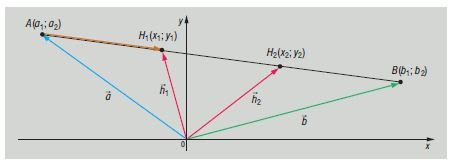
\includegraphics[width=0.8\linewidth]{Harmad}
		\end{figure}
	\end{theorem}
	\begin{theorem}
		Az $AB$ szakaszt $p:q$ arányban osztó pont koordinátái: $R\left(\frac{qa_1+pb_1}{p+q};\frac{qa_2+pb_2}{p+g}\right)$
	\end{theorem}
\section{Egyenest meghatározó adatok}
	Egy egyenest egyértelműen meghatároz 2 pontja, vagy 1 pontja, és 1, az állását jellemző adata. Ilyen adat például az irányvektora, normálvektora, irányszöge, iránytangense.
	\begin{definition}
		Az egyenes irányvektora az egyenessel párhuzamos, nullvektortól különböző vektor. Jele: $\vec{v}(v_1;v_2)$.
	\end{definition}
	\begin{definition}
		Az egyenes normálvektora az egyenesre merőleges, nullvektortól különböző vektor. Jele: $\vec{n}(A;B)$.
	\end{definition}
	\begin{definition}
		Az egyenes irányszöge az a $-\frac{\pi}{2}<\alpha\le\frac{\pi}{2}$ szög, amelyet az egyenes az $x$ tengely pozitív irányával bezár.
	\end{definition}
	\begin{definition}
		Az egyenes irányszögének tangensét (ha létezik) az egyenes iránytangensének nevezzük. Jele: $m=\text{tg}\alpha$. Az $\alpha=90\degree$-os irányszögű egyenesnek nincs iránytangense.
	\end{definition}
	\begin{outline}
		\1 Összefüggések
			\2 $\vec{v}(v_1;v_2)$ irányvektor $\implies \vec{n}(-v_2;v_1)\vee\vec{n}(v_2;-v_1)$ normálvektor, $m=\frac{v_2}{v_1}=\text{tg}\alpha\ (v_1\ne0)$
			\2 $\vec{n}(A;B)$ normálvektor $\implies\vec{v}{-B;A}\vee\vec{v}(B;-A)$ irányvektor, $m=-\frac{A}{B}=\text{tg}\alpha\ (B\ne0)$
			\2 Iránytangens $m\implies$ irányszög: $\alpha=\text{arctg}\ m$, irányvektor: $\vec{v}(1;m)$, normálvektor: $\vec{n}(-m;1)\vee\vec{n}(m;-1)$
			\2 Irányszög $\alpha\implies$ iránytangens: $m=\text{tg}\alpha\implies$ irányvektor: $\vec{v}(1;\text{tg}\alpha)$, normálvektor: $\vec{n}(-\text{tg}\alpha;1)\vee\vec{n}(\text{tg}\alpha;-1)$. Ha $\alpha=90\degree$, akkor $m$ nem létezik, $\vec{v}(0;1)$, és $\vec{n}(1;0)$.
			\2 Egyenes két különböző pontja $A(a_1;a_2)$ és $B(b_1;b_2)$, akkor:
				\3 Irányvektor: $\overrightarrow{AB}=\vec{v}(b_1-a_1;b_2-a_2)$
				\3 Normálvektor: $\vec{n}(a_2-b_2;b_1-a_1)\vee\vec{n}(b_2-a_2;a_1-b_1)$
				\3 Iránytangens: $m=\frac{b_2-a_2}{b_1-a_1}$
				\3 Irányszög: $\alpha=\text{arctg}\ m$
	\end{outline}
\section{Egyenes egyenletei}
	\begin{definition}
		Egy alakzat egyenletén, a síkbeli $xy$ koordináta-rendszerben, olyan egyenletet értünk,
		melyet az alakzat pontjainak koordinátái kielégítenek, de más síkbeli pontok nem.
	\end{definition}
	\begin{theorem}
		Ha egy egyenesnek adott a $P_0(x_0;y_0)$ pontja, és egy $\vec{n}(A;B)$ normálvektora, akkor az egyenes normálvektoros egyenlete: $Ax+By=Ax_0+By_0$.
	\end{theorem}
	\begin{proof}
		Egy $P(x;y)$ pont akkor és csak akkor van rajta az $e$ egyenesen, ha a $\overrightarrow{P_0P}$ vektor merőleges az egyenes $\vec{n}(A;B)$ normálvektorára. Jelölje $P_0$ pont helyvektorát $\vec{r_0}$, a $P$ pont helyvektorát $\vec{r}$, akkor $\overrightarrow{P_0P}=\vec{r}-\vec{r_0}$, koordinátákkal: $\overrightarrow{P_0P}=(x-x_0;y-y_0)$. $\overrightarrow{P_0P}$ akkor és csak akkor merőleges az egyenes normálvektorára, ha $\overrightarrow{P_0P}\centerdot\vec{n}$=0, azaz: $(x-x_0)*A+(y-y_0)*B=0$, átrendezve:
		\begin{equation*}
			Ax+By=Ax_0+By_0
		\end{equation*}
	\end{proof}
	\begin{theorem}
		Ha egy egyenesnek adott a $P_0(x_0;y_0)$ pontja és egy $\vec{v}(v_1;v_2)$ irányvektora, akkor az egyenes irányvektoros egyenlete: $v_2x-v_1y=v_2x_0-v_1y_0$
	\end{theorem}
	\begin{theorem}
		Ha adott az $y$ tengellyel nem párhuzamos egyenes egy $P_0(x_0;y_0)$ pontja és $m$ iránytangense, akkor iránytényezős egyenlete: $y-y_0=m*(x-x_0)$
	\end{theorem}
	\begin{theorem}
		Az $y$ tengellyel párhuzamos, $P_0(x_0;y_0)$ ponton átmenő egyenes egyenlete: $x=x_0$
	\end{theorem}
	\begin{definition}
		Két egyenes metszéspontja egy olyan pont, amely illeszkedik mindkét egyenesre
	\end{definition}
	\begin{definition}
		Két egyenes hajlásszöge irányvektoraik, vagy normálvektoraik szöge.
	\end{definition}
\section{Két egyenes merőlegessége és párhuzamossága}
	Legyen két egyenes $e$ és $f$, irányvektoraik $\vec{v}_e$ és $\vec{v}_f$, normálvektoraik $\vec{n}_e$ és $\vec{n}_f$, irányszögeik $\alpha_e$ és $\alpha_f$, iránytangenseik $m_e$ és $m_f$, ha léteznek.
	\begin{outline}
		\1 $e\|f\Leftrightarrow$
			\2[] $\vec{v_e}\|\vec{v_f},\text{ azaz }\exists\lambda\in\mathbb{R}\setminus\{0\}\ \vec{v_e}=\lambda*\vec{v_f}$
			\2[] $\vec{n_e}\|\vec{n_f},$ azaz $\exists\lambda\in\mathbb{R}\setminus\{0\}\ \vec{n_e}=\lambda*\vec{v_f}$
			\2[] $\alpha_e=\alpha_f$
			\2[] $m_e=m_f$
		\1 $e\perp f\Leftrightarrow$
			\2[] $\vec{v_e}\perp \vec{v_f},$ azaz $\vec{v_e}\centerdot\vec{v_f}=0$
			\2[] $\vec{n_e}\perp \vec{n_f},$ azaz $\vec{n_e}\centerdot\vec{n_f}=0$
			\2[] $\vec{n_e}=\lambda*\vec{v_f}\ (\lambda\ne0)$
			\2[] $\vec{v_e}=\lambda*\vec{n_f}\ (\lambda\ne0)$
			\2[] $m_e*m_f=-1$
	\end{outline}
\section{Elsőfokú egyenlőtlenségek}
	\begin{definition}
		Elsőfokú egyismeretlenes egyenlőtlenség: $ax+b>0 (a\ne0)$
	\end{definition}
	\begin{equation*}
		\begin{cases*}
			a>0,& akkor $x>-\frac{b}{a}$\\
			a<0,& akkor $x<-\frac{b}{a}$
		\end{cases*}
	\end{equation*}
	Ha megengedett az egyenlőtlenség, akkor megengedett a megoldásban is.
	\begin{definition}
		Elsőfokú kétismeretlenes egyenlőtlenség: $ax+by+c>0 (a\ne0)$
	\end{definition}
	\begin{equation*}
		\begin{cases*}
			b>0,& akkor $y>-\frac{a}{b}x-\frac{c}{b}$\\
			b<0,& akkor $y<-\frac{a}{b}x-\frac{c}{b}$\\
			b=0,& akkor $ax+c>0$ egyismeretlenes egyenlőtlenség
		\end{cases*}
	\end{equation*}
\section{Alkalmazások}
	\begin{outline}
		\1 Adott tulajdonságú ponthalmazok keresése
		\1 Elemi geometriai problémák egyszerűbb megoldása. Pl.: a háromszög magasságvonalai egy pontban metszik egymást.
	\end{outline}
\section{Matematikatörténet}
	\begin{outline}
		\1 Descartes (XVII. század)
			\2 Geometria című könyve: első koordináta-geometriai mű
		\1 Cavalieri (XVII. század)
			\2 Polárkoordináták: $r,\alpha$
	\end{outline}
\chapter{Kör és parabola}
\section{Kör és egyenlete}
	\begin{definition}
		A kör azon pontok halmaza a síkon, amelyek egy adott ponttól adott távolságra vannak.
		Az adott pontot a kör középpontjának, az adott távolságot a kör sugarának nevezzük.
	\end{definition}
	\begin{definition}
		Ha egy mindkét irányban végtelen egyenes körkúpfelületet, egy a tengelyére merőleges síkkal elmetszünk, akkor kört kapunk.
	\end{definition}
	\begin{theorem}
		A $C(u;v)$ középpontú $r$ sugarú kör egyenlete $(x-u)^2+(y-v)^2=r^2$
	\end{theorem}
	A kör egyenlete kétismeretlenes másodfokú egyenlet, mivel átalakítható: $x^2+y^2-2ux-2vy+u^2+v^2-r^2=0$, azaz
	\begin{equation*}
		x^2+y^2+Ax+By+C=0
	\end{equation*}
	alakra hozható, ahol $A;B;C\in\mathbb{R}\wedge A^2+B^2-4C>0$. Ekkor a kör középpontjának koordinátáira:
	\begin{align*}
		A&=-2u\implies u=-\frac{A}{2}\\
		B&=-2v\implies v=-\frac{B}{2}
	\end{align*}
	Illetve:
	\begin{align*}
		u^2+v^2-r^2=C&\implies r^2=u^2+v^2-C\implies r^2=\frac{A^2+B^2-4C}{4}\implies \\&\implies r=\frac{\sqrt{A^2+B^2-4C}}{2}
	\end{align*}
\section{Parabola és egyenletei}
	\begin{definition}
		A parabola azon pontok halmaza a síkon, amelyek a sík egy $v$ egyenesétől és az egyenesre
		nem illeszkedő $F$ ponttól egyenlő távolságra vannak. Az egyenes a parabola direktrixe (vezéregyenese), a pont a parabola fókuszpontja.
	\end{definition}
	A direktrix és a fókuszpont távolsága a parabola paramétere ($p>0$). A fókuszpontra illeszkedő, a direktrixre merőleges egyenes a parabola szimmetriatengelye, vagy tengelye (t). A parabola tengelyen lévő pontja a parabola tengelypontja (T). A tengelypont felezi a fókuszpont és a direktrix távolságát.
	\begin{definition}
		Ha egy mindkét irányban végtelen egyenes körkúpfelületet, egy olyan síkkal elmetszünk, amely a kúp pontosan egy alkotójával párhuzamos, parabolát kapunk.
	\end{definition}
	\begin{figure}[H]
		\centering
		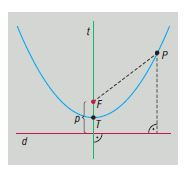
\includegraphics[width=0.4\linewidth]{Par}
	\end{figure}
	\begin{theorem}
		Az $F\left(0;\frac{p}{2}\right)$ fókuszpontú $y=-\frac{p}{2}$ direktrixű parabola egyenlete: $y=\frac{1}{2p}x^2$.
	\end{theorem}
	\begin{proof}
		\begin{figure}[H]
			\centering
			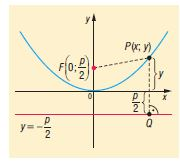
\includegraphics[width=0.4\linewidth]{ParBiz}
		\end{figure}
		A $P(x;y)$ pont és a direktrix távolsága a $PQ$ távolság, ahol $Q$ P merőleges vetülete a direktrixen, ezért $Q\left(x;-\frac{p}{2}\right)$.
		\begin{equation*}
			\begin{rcases*}
				PQ=\sqrt{(x-x)^2+\left(y+\frac{p}{2}\right)^2}=\sqrt{\left(y+\frac{p}{2}\right)^2}\\
				PF=\sqrt{(x-0)^2+\left(y-\frac{p}{2}\right)^2}=\sqrt{x^2+\left(y-\frac{p}{2}\right)^2}
			\end{rcases*}
			PQ=PF
		\end{equation*}
		\begin{align*}
			\sqrt{\left(y+\frac{p}{2}\right)^2}&=\sqrt{x^2+\left(y-\frac{p}{2}\right)^2}\tag{Mivel mindkét oldal nemnegatív, a négyzetre emelés ekvivalens átalakítás}\\
			y^2+py+\frac{p^2}{4}&=x^2+y^2-py+\frac{p^2}{4}\\
			y&=\frac{1}{2p}x^2
		\end{align*}
	\end{proof}
	\begin{theorem}
		$p$ paraméterű $T(u;v)$ tengelypontú parabolák egyenletei, és jellemzőik:
		\begin{figure}[H]
			\centering
			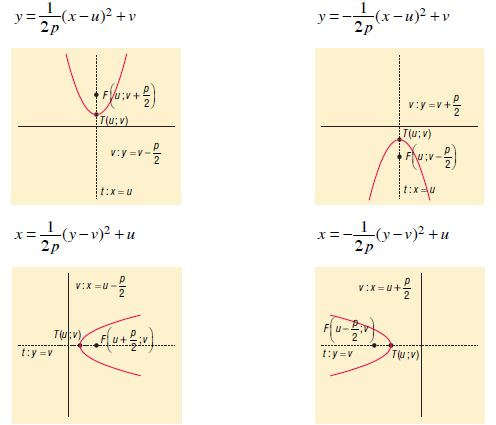
\includegraphics[width=0.8\linewidth]{ParEgy}
		\end{figure}
	\end{theorem}
	Minden másodfokú függvény grafikonja az y tengellyel párhuzamos tengelyű parabola, és minden y tengellyel párhuzamos tengelyű parabola valamelyik másodfokú függvény grafikonja.
\section{Kör és egyenes kölcsönös helyzete}
	Egy síkban egy körnek és egy egyenesnek háromféle helyzete lehet: nincs közös pontjuk, egy közös pontjuk van (az egyenes érinti a kört), két közös pontjuk van (az egyenes metszi a kört).
	\begin{figure}[H]
		\centering
		\includegraphics[width=0.8\linewidth]{KörEgy}
	\end{figure}
	\begin{outline}
		\1 Közös pontok meghatározása: egyenleteikből álló egyenletrendszerből
			\2 Egyenes egyenletből egyik ismeretlen kifejezése
			\2 Kör egyenletébe helyettesítés -> másodfokú egyismeretlenes egyenlet
			\2 Diszkrimináns adja meg közös pontok számát
	\end{outline}
\section{Parabola és egyenes kölcsönös helyzete}
	Közös pontok száma lehet 2, 1, 0.
	\begin{figure}[H]
		\centering
		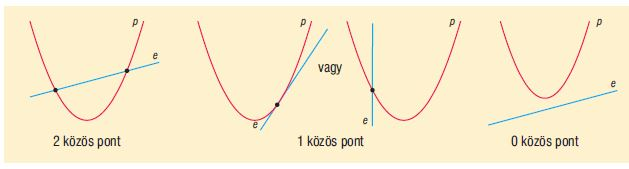
\includegraphics[width=\linewidth]{ParEgye}
	\end{figure}
	\begin{definition}
		A parabola érintője olyan egyenes, melynek egy közös pontja van a parabolával és
		nem párhuzamos a parabola tengelyével.
	\end{definition}
	\begin{outline}
		\1 Érintő meghatározása
			\2 Egyenes egyenletét $m$ meredekséggel felírva
				\3 $m$ ne tengellyel párhuzamos egyenesre utaljon
			\2 Egyenletrendszernek egy megoldása van
			\2 Parabola egyenletéből egyenes egyenletébe helyettesítés
				\3 Másodfokú egyenlet diszkriminánsa 0
		\1 Deriválás
			\2 Az $y$ tengellyel párhuzamos: másodfokú függvény deriváltja egyenes meredeksége
			\2 Általános eset: implicit deriválás, $y'$-ra rendezés adja az egyenes meredekségét, ha nem párhuzamos az $y$ tengellyel
	\end{outline}
\section{Másodfokú egyenlőtlenségek}
	\begin{definition}
		Egyenlőtlenség algebrai kifejezések a $<,>,\le,\ge$ jelek valamelyikével való összekapcsolása. Ha a kifejezések másodfokúak, másodfokú egyenlőtlenségről beszélünk.
	\end{definition}
	\begin{outline}
		\1 Megoldási módszerek hasonlóak az egyenlethez
			\2 Mérlegelv: Negatív értékkel való szorzás/osztásnál irány fordul
			\2 Reciprok: Ha mindkét oldal negatív irány fordul
			\2 Grafikus megoldás:
				\3 Másodfokú kifejezések grafikonja parabola
				\3 0-ra rendezés, $a>0$
				\3 Bal oldali kifejezés ábrázolása
				\3 Zérushelyek megállapítása
				\3 2 zérushely
				\begin{figure}[H]
					\centering
					\begin{tabular}{cc}
						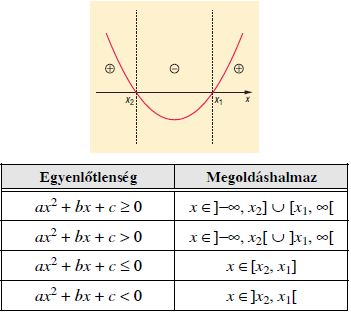
\includegraphics[width=0.5\linewidth]{2}&
						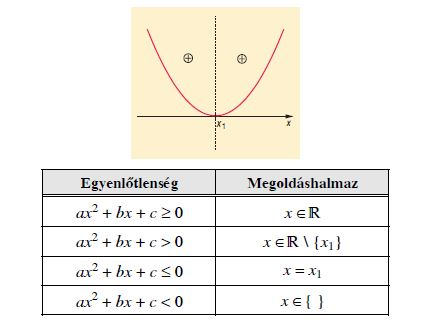
\includegraphics[width=0.5\linewidth]{1}\\
						\multicolumn{2}{c}{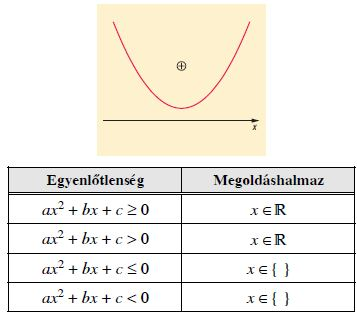
\includegraphics[width=0.5\linewidth]{0}}
					\end{tabular}
				\end{figure}
	\end{outline}
\section{Alkalmazások}
	\begin{outline}
		\1 Geometriai feladatok megoldása algebrai úton
			\2 Szélsőérték-feladatok
			\2 Adott tulajdonságú ponthalmaz keresése
	\end{outline}
\section{Matematikatörténet}
	\begin{outline}
		\1 Descartes (XVII. század)
			\2 Geometria című könyve: első koordináta-geometriai mű
		\1 Galileo (XVI-XVII. század)
			\2 Lövedék pályája parabola, ha csak gravitáció hat rá
	\end{outline}
\chapter{Térgeometria}
\section{Térelemek}
	Pont, egyenes, sík alapfogalmak, nem definiáljuk őket.
	\begin{definition}
		Két térelem illeszkedő, ha egyik részhalmaza a másiknak
	\end{definition}
	\begin{definition}
		Két egyenes párhuzamos, ha egy síkban vannak és nem metszik egymást.
	\end{definition}
	\begin{definition}
		Egyenes és sík, illetve 2 sík párhuzamos, ha nincs közös pontjuk.
	\end{definition}
	\begin{definition}
		Egy síkban két, azonos pontból kiinduló félegyenest és az általuk meghatározott bármelyik síkrészt szögnek nevezzük. A közös kezdőpont a szög csúcspontja, a két félegyenes a szög szárai, a síkrész a szögtartomány.
	\end{definition}
	\begin{definition}
		Illeszkedő vagy párhuzamos térelemek szöge 0\degree
	\end{definition}
	\begin{definition}
		Két metsző egyenes 4 szöget alkot, ezek közül 2-2 egyenlő. Ha a két egyenes nem merőleges egymásra, akkor a két egyenes hajlásszöge a kétfajta szög közül a kisebbik. Ha a két egyenes merőleges egymásra, akkor a hajlásszögük derékszög.
	\end{definition}
	\begin{definition}
		Két egyenes kitérő, ha nincsenek egy síkban.
	\end{definition}
	\begin{definition}
		Két kitérő egyenes hajlásszöge egyenlő a tér egy tetszőleges pontján átmenő és az adott egyenesekkel párhuzamos egyenesek hajlásszögével.
	\end{definition}
	\begin{theorem}
		Egy, a síkot metsző egyenes merőleges a síkra, ha merőleges a sík minden egyenesére.
	\end{theorem}
	\begin{definition}
		Ha az $e$ egyenes nem merőleges a síkra, akkor az egyenes merőleges vetülete a síkon
		szintén egyenes $(e')$. Ebben az esetben az egyenes és a sík hajlásszögén az egyenes és a vetülete hajlásszögét értjük.
	\end{definition}
	\begin{definition}
		Ha két sík nem párhuzamos egymással, akkor metszésvonaluk egy pontjában mindkét síkban merőlegest állítunk a metszésvonalra. A két sík hajlásszöge e két egyenes hajlásszögével egyenlő.
	\end{definition}
	\begin{definition}
		Két illeszkedő, vagy metsző térelem távolsága 0.
	\end{definition}
	\begin{definition}
		Két pont távolsága a pontokat összekötő szakasz hossza.
	\end{definition}
	\begin{definition}
		Pont és egyenes távolsága a pontból az egyenesre bocsátott merőleges szakasz hossza.
	\end{definition}
	\begin{definition}
		Pont és sík távolsága a pontból a síkra bocsátott merőleges szakasz hossza.
	\end{definition}
	\begin{definition}
		Párhuzamos egyenesek távolsága: bármelyik egyenes egy tetszőleges pontjának távolsága
		a másik egyenestől.
	\end{definition}
	\begin{definition}
		Két kitérő egyenes távolsága az őket összekötő, mindkettőre merőleges szakasz hossza. Normáltranszverzális az az egyenes, amely mindkét kitérő egyenesre merőleges
	\end{definition}
	\begin{definition}
		Egyenes és vele párhuzamos sík távolsága az egyenes egy tetszőleges pontjának
		a síktól való távolságával egyenlő.
	\end{definition}
	\begin{definition}
		Két párhuzamos sík távolsága az egyik sík egy tetszőleges pontjának a másik síktól vett
		távolsága.
	\end{definition}
\section{Térbeli alakzatok}
	\begin{definition}
		A térnek véges felületekkel határolt részét testnek nevezzük.
	\end{definition}
	\begin{definition}
		A sokszöglapokkal határolt testek a poliéderek.
	\end{definition}
	\begin{definition}
		A szabályos testek olyan poliéderek, amelynek lapjai egybevágó szabályos sokszögek,
		valamennyi lapszögük és élszögük egyenlő.
	\end{definition}
	\begin{figure}[H]
		\centering
		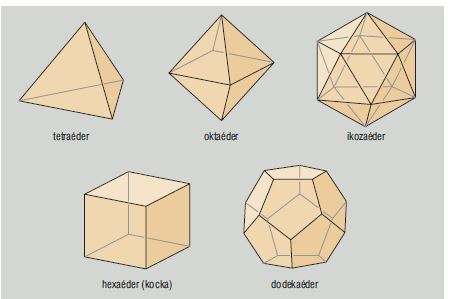
\includegraphics[width=0.9\linewidth]{SzabPoli}
	\end{figure}
	\begin{definition}[Hengerszerű testek]
		Egy síkidom kerületén levő pontokon keresztül párhuzamosokat húzunk egy, a síkidom síkjával nem párhuzamos egyenessel. Az így kapott palástfelületet az eredeti síkidom síkjával és egy vele párhuzamos síkkal elmetszünk. Ha a test alaplapja sokszög, akkor hasábnak, ha kör, hengernek nevezzük. Ha a párhuzamos egyenesek merőlegesek az alaplap síkjára, akkor a testet egyenes hengerszerű testnek, különben ferde hengerszerű testnek nevezzük.
	\end{definition}
	\begin{definition}[Kúpszerű testek]
		Egy síkidom kerületén levő pontokon keresztül egyeneseket húzunk egy, a síkidom síkjára nem illeszkedő ponton keresztül. Ha a test alaplapja sokszög, akkor gúlának, ha kör, kúpnak nevezzük. Ha a kúp minden alkotója (az egyenesek az adott pont és a síkidom közti szakasza) egyenlő hosszú, akkor egyenes kúpszerű testnek, különben ferde kúpszerű testnek nevezzük.
	\end{definition}
	\begin{definition}[Csonkakúpszerű testek]
		Ha egy kúpszerű testet az alaplapjával párhuzamos síkkal elmetszünk, akkor a két párhuzamos sík közti testet csonkakúpszerű testnek nevezzük. Ha a test alaplapja sokszög, akkor csonkagúlának, ha kör, csonkakúpnak nevezzük.
	\end{definition}
	\begin{definition}[Gömbfelület]
		Egy adott ponttól egyenlő távolságra levő pontok halmaza a térben. Gömböt kapunk, ha egy kört valamelyik átmérője mentén megforgatunk.
	\end{definition}
\section{Testek felszíne}
	A felszín jele: $A$. Poliéderek felszíne a poliédert határoló véges számú sokszöglap területének az összege. Egyébként:
	\begin{itemize}
		\item Ha a test felülete síkba kiteríthető, akkor ennek a kiterített felületnek a területe adja a test felszínét (pl. henger, kúp).
		\item Ha csak egy olyan pozitív valós szám van, amely a test által tartalmazott poliéderek felszínénél nem kisebb, és a testet tartalmazó poliéderek felszínénél nem nagyobb, akkor az a test felszíne.
	\end{itemize}
	\begin{theorem}[Forgástest]
		Ha az $f(x)$ függvény az $[a;b]$ intervallumon folytonos és $f(x)\ge0$, akkor az $f(x)$ függvény grafikonjának az $x$ tengely körüli megforgatásával keletkezett forgástest palástjának felszíne:
		\begin{equation*}
			A=2\pi\int_{a}^{b}f(x)*\sqrt{1+\left(f'(x)\right)^2}
		\end{equation*}
		A teljes forgástest felszíne megegyezik a palást felszínének, és a fedő- illetve alaplap területének összegével.
	\end{theorem}
	\begin{theorem}
		Hasonló testek felszínének aránya megegyezik a hasonlóság arányának négyzetével.
	\end{theorem}
\section{Testek térfogata}
	A térfogat jele: $V$. Poliéder térfogata poliéderre jellemző pozitív szám, amely axiómái a következők:
	\begin{itemize}
		\item Egységkocka térfogata 1
		\item Egybevágó poliéderek térfogata egyenlő
		\item Egy részpoliéderekre szétvágott poliéder térfogata egyenlő a részek térfogatának összegével
	\end{itemize}
	Poliéderektől különböző testeknél ha egyetlen olyan pozitív valós szám van, amely a test által tartalmazott poliéderek térfogatánál nem kisebb, és a testet tartalmazó poliéderek térfogatánál nem nagyobb, akkor ezt a számot a test térfogatának nevezzük.
	\begin{theorem}[Forgástest]
		Ha az $f(x)$ függvény az $[a;b]$ intervallumon folytonos és $f(x)\ge0$, akkor az $f(x)$ függvény grafikonjának az $x$ tengely körüli megforgatásával keletkezett forgástest térfogata:
		\begin{equation*}
			V=\pi\int_{a}^{b}f^2(x)dx
		\end{equation*}
	\end{theorem}
	\begin{theorem}
		Az $r$ sugarú gömb térfogata: $V=\frac{4}{3}r^3\pi$
	\end{theorem}
	\begin{proof}
		A gömb egy félkör átmérő körüli megforgatása, ezért térfogata, mivel az $r$ sugarú kör egyenletéből $y^2=\sqrt{r^2-x^2}$:
		\begin{align*}
		V&=\pi\int_{-r}^{r}\left(r^2-x^2\right)dx=\pi*\left[r^2x-\frac{x^3}{3}\right]^r_{-r}=\pi*
		\left(r^3-\frac{r^3}{3}-\left(-r^3+\frac{-r^3}{3}\right)\right)=\\
		&=\pi*\left(2r^3-\frac{2r^3}{3}\right)=\pi*\frac{4r^3}{3}
		\end{align*}
	\end{proof}
	\begin{theorem}
		Hasonló testek térfogatának aránya megegyezik a hasonlóság arányának köbével.
	\end{theorem}
\section{Testek felszíne és térfogata}
	\begin{figure}[H]
		\centering
		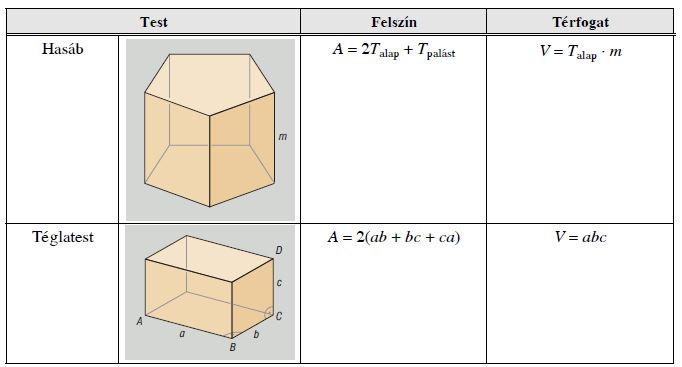
\includegraphics[width=.8\linewidth]{Test1}
	\end{figure}
	\begin{figure}[H]
		\centering
		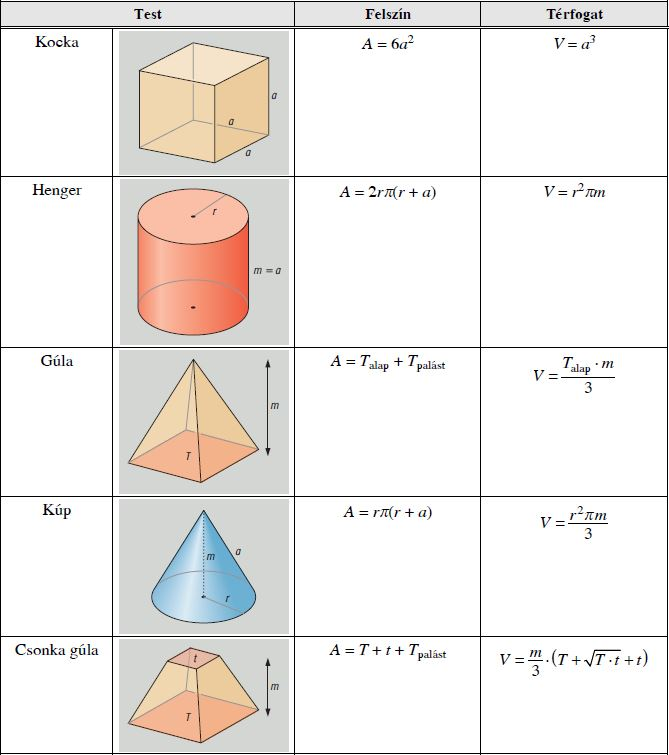
\includegraphics[width=.8\linewidth]{Test2}
		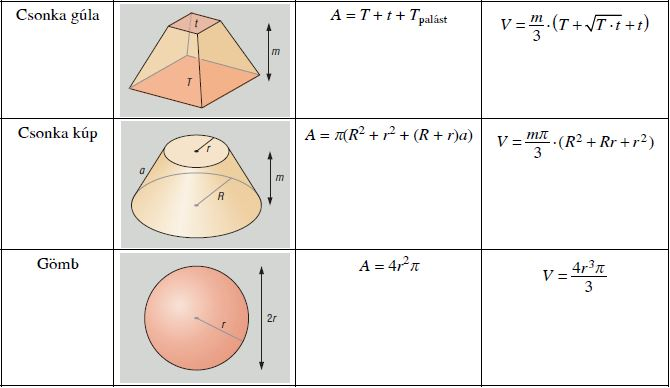
\includegraphics[width=.8\linewidth]{Test3}
	\end{figure}
	\begin{theorem}
		Egy $r$ sugarú, $a$ alkotójú kúp felszíne $A=r\pi(r+a)$
	\end{theorem}
\section{Alkalmazások}
	\begin{outline}
		\1 Geometriai valószínűség számítása
		\1 Térképészet, földmérés: távolságmérés, szögmérés
		\1 Építészmérnöki munka: távolságmérés, szögmérés, felszín, térfogatszámítás
	\end{outline}
\section{Matematikatörténet}
	\begin{outline}
		\1 Császár Ákos (XX. század)
			\2 Poliéder, bármely két csúcspontja szomszédos
				\3 7 csúcs, 14 háromszöglap, 21 él
		\1 Szilassi Lajos (XX. század)
			\2 Test, 7 lapja van, bármely 2 szomszédos
	\end{outline}
\chapter{Terület}
\section{Területszámítás}
	\begin{definition}
		A terület minden síkidomhoz rendelt pozitív valós szám, amelynek axiómái:
		\begin{itemize}
			\item Egységnyi oldalhosszúságú négyzet területe egységnyi
			\item Egybevágó síkidomok területe egyenlő
			\item Ha egy síkidomot véges számú síkidomra darabolunk, akkor az egyes részek területének összege egyenlő az eredeti sokszög területével
		\end{itemize}
	\end{definition}
\section{Síkidomok területe}
	\begin{theorem}
		Téglalap területe két szomszédos oldalának szorzatával egyenlő: $T=a*b$
	\end{theorem}
	\begin{theorem}
		Paralelogramma területe: $T=a*m_a$
	\end{theorem}
	\begin{theorem}
		Háromszög területe: 
		\begin{equation*}
		T=\frac{a*m_a}{2}=\frac{a*b*\sin\gamma}{2}=r*s=\frac{a*b*c}{4R}=\sqrt{s(s-a)(s-b)(s-c)}
		\end{equation*}
		Ahol $r$ beírt kör sugara, $R$ körülírt kör sugara, $s$ a félkerület.
	\end{theorem}
	\begin{theorem}
		A trapéz területe az alapok számtani közepének és a trapéz magasságának szorzata:
		\begin{equation*}
			T=\frac{a+c}{2}*M
		\end{equation*}
	\end{theorem}
	\begin{theorem}
		Bármely sokszög véges számú háromszögre darabolható, területe megegyezik ezeknek a háromszögeknek a területösszegével.
	\end{theorem}
	\begin{theorem}
		Négyszög területe az átlói hossza és az átlók által bezárt szög szinuszának a szorzatának a fele:
		\begin{equation*}
			T=\frac{e*f*\sin\varphi}{2}
		\end{equation*}
	\end{theorem}
	\begin{theorem}
		Deltoid területe átlói szorzatának a fele.
	\end{theorem}
	\begin{theorem}
		Szabályos n-szög területe:
		\begin{equation*}
			T=n*\frac{a*r}{2}=n*\frac{R^2*\sin\frac{360\degree}{n}}{2}
		\end{equation*}
		Ahol $r$ a beírt kör sugara, $R$ a körülírt kör sugara.
	\end{theorem}
	\begin{theorem}
		$r$ sugarú kör területe: $r^2\pi$.
	\end{theorem}
\section{Határozott integrál}
	\begin{definition}
		Görbe alatti terület egy $[a;b]$ intervallumon folytonos, korlátos, pozitív értékű $f$ függvény görbéjének az intervallumhoz tartozó íve, az $x=a$, az $x=b$ egyenesek és az $x$ tengely által határolt terület.
	\end{definition}
	\begin{figure}[H]
		\centering
		\includegraphics[width=.3\linewidth]{GörT}
	\end{figure}
	\begin{definition}
		Ha az $[a;b]$ intervallumot az $a=x_0,x_1,\dots,x_n=b$ pontokkal $n$ részre osztjuk, akkor ezt az intervallum egy felosztásának nevezzük.
	\end{definition}
	\begin{outline}
		\1 Felosztás intervalluma: $[x_{i-1};x_i]$. 
			\2 $m_i=\inf f(x),$ ha $x\in[x_{i-1};x_i]$
			\2 $M_i=\sup f(x),$ ha $x\in[x_{i-1};x_i]$
			\2 Intervallum fölé téglalapok, másik oldaluk $m_i$, $M_i$
			\begin{figure}[H]
				\centering
				\includegraphics[width=.3\linewidth]{Tégl}
			\end{figure}
			\2 Felosztás minden intervallumához
			\2 Kisebb/nagyobb téglalapok -> sokszög
			\2 Beírt/körülírt sokszög
			\2 Beírt sokszög területe: alsó közelítő összeg:
			\begin{equation*}
				s_n=\sum_{i=1}^{n} m_i*(x_i-x_{i-1})
			\end{equation*}
			\2 Körülírt sokszög területe: felső közelítő összeg:
			\begin{equation*}
				S_n=\sum_{i=1}^n M_i*(x_i-x_{i-1})
			\end{equation*}
			\2 Felosztás finomítása: további osztópontok
	\end{outline}
	\begin{definition}
		Az $[a;b]$ intervallumon korlátos $f$ függvény integrálható, ha bármely minden határon túl finomodó felosztássorozatnak közös határértéke van, azaz $\lim\limits_{n\to\infty} s_n=\lim\limits_{n\to\infty}S_n$. Ez a közös határérték az $f$ függvény $[a;b]$ intervallumon vett határozott integrálja. Jelölés:
		\begin{equation*}
			\int_{a}^{b}f(x)dx
		\end{equation*}
	\end{definition}
	\begin{theorem}
		Ha $f$ integrálható, akkor:
		\begin{enumerate}
			\item $\int_{b}^{a}f(x)dx=-\int_{a}^{b}f(x)dx$
			\item $\int_{a}^{a}f(x)dx=0$
			\item $\int_{a}^{b}k*f(x)dx=k\int_{a}^{b}f(x)dx$
			\item $\int_{a}^{b}(f(x)\pm g(x))dx=-\int_{a}^{b}f(x)dx\pm\int_{a}^{b}g(x)dx$
			\item $\int_{a}^{b}f(x)dx+\int_{b}^{c}f(x)dx=\int_{a}^{c}f(x)dx$
			\item $\min f(x)*(b-a)\le\int_{a}^{b}f(x)dx\le\max f(x)*(b-a)$
			\item $f(x)\ge g(x)$ $[a;b]$-n $\implies\int_{a}^{b}f(x)dx\ge\int_{a}^{b}g(x)dx$
		\end{enumerate}
	\end{theorem}
	\begin{theorem}[Középértéktétel]
		Ha $f$ folytonos $[a;b]$-n, akkor
		\begin{equation*}
			\exists c\in[a;b]\ f(c)=\frac{1}{b-a}\int_{a}^{b}f(x)dx
		\end{equation*}
	\end{theorem}
	\begin{theorem}
		Ha $f$ folytonos $[a;b]$-n, akkor $F(x)=\int_{a}^{x}f(t)dt$ is folytonos $[a;b]$-n, differenciálható $(a;b)$-n és deriváltja $f(x)$:
		\begin{equation*}
			F'(x)=\frac{d}{dx}\int_{a}^{x}f(t)dt=f(x)
		\end{equation*}
	\end{theorem}
	\begin{proof}
		Alkalmazzuk a derivált definícióját $F(x)$-re:
		\begin{align*}
			F'(x)&=\frac{F(x+h)-F(x)}{h}=\frac{\int_{a}^{x+h}f(t)dt-\int_{a}^{x}f(t)dt}{h}=\frac{\int_{x}^{x+h}f(t)dt}{h}=\frac{1}{h}*\int_{x}^{x+h}f(t)dt=\tag{Középértéktétel miatt}\\
			&=f(c)
		\end{align*}
		Mivel $h\to0$, és $c\in[x;x+h]$, $c\to x$. Mivel $f$ folytonos:
		\begin{equation*}
			\lim\limits_{h\to0}f(c)=f(x)
		\end{equation*}
		Az eddigiekből következik, hogy:
		\begin{equation*}
		\frac{dF}{dx}=f(x)
		\end{equation*}
	\end{proof}
	\begin{theorem}[Newton-Leibniz tétel]
		Ha $f$ folytonos $[a;b]$ minden pontjában, és $F$ $f$ primitív függvénye $[a;b]$-n, akkor:
		\begin{equation*}
			\int_{a}^{b}f(x)dx=F(b)-F(a)
		\end{equation*}
	\end{theorem}
\section{Görbe alatti terület}
	\begin{theorem}
		Ha az $[a;b]$-n folytonos $f$ függvény nem vált előjelet, akkor $x=a,\ x=b,$ az $x$ tengely, és a függvény grafikonja által közrezárt síkidom területe: $T=\left|\int_{a}^{b}f(x)dx\right|$
	\end{theorem}
	\begin{theorem}
		Két függvény által közrezárt síkidom területe:
		\begin{equation*}
			T=\int_{a}^{b}(f(x)-g(x))dx\tag{ha $f(x)>g(x)$}
		\end{equation*}
	\end{theorem}
\section{Alkalmazások}
	\begin{outline}
		\1 Pitagorasz tétel bizonyítása terület-összerakással
		\1 Geometriai valószínűség kiszámítása
		\1 Síkidomokkal, síkba kiteríthető felületekkel határolt testek felszínének meghatározása
	\end{outline}
\section{Matematikatörténet}
	\begin{outline}
		\1 Newton, Leibniz (XVII-XVIII. század)
			\2 Egymástól függetlenül felfedezték a differenciál- és integrálszámítást
			\2 Jelölések többnyire Leibniztől származnak
	 	\1 Riemann (XIX. század)
	 		\2 Riemann-integrál kifejlesztése
 		\1 Lebesgue (XIX-XX. század)
 			\2 Lebesgue-integrál kifejlesztése
 			\2 Riemann-integrál általánosítása
 			\2 $D(x)=\begin{cases}
	 			0, & \text{ ha } x\in\mathbb{Q}\\
	 			1, & \text{ ha } x\in\mathbb{Q}^*
 			\end{cases}$
		 	\2 $\int_{[0;1]} D(x)d\mu=1$
		 		\3 $\mu$ - Lebesgue-mérték
	\end{outline}
\chapter{Valószínűségszámítás 1.}
\section{Kombinációk}
	A kombinatorika, a valószínűség-számítás és a matematikai statisztika a véletlen tömegjelenségek
	törvényszerűségével foglalkozik. A kombinatorika tárgyát képezik a sorba rendezési és a részhalmaz
	kiválasztási problémák, a kombinatorika rendszerint dolgok megszámlálásával foglalkozik.
	\begin{definition}
		Van $n$ egymástól különböző elemünk. Ha ezekből $k\le n$ db-ot kiválasztunk úgy, hogy az elemek sorrendjére nem vagyunk tekintettel, akkor $n$ elem $k$-ad osztályú ismétlés nélküli kombinációját kapjuk.
	\end{definition}
	\begin{theorem}
		$n$ elem $k$-ad osztályú ismétlés nélküli kombinációinak száma:
		\begin{equation*}
			\binom{n}{k}=\frac{n!}{k!*(n-k)!}
		\end{equation*}
	\end{theorem}
	\begin{definition}
		Ha $n$ különböző elemből kell $k$ elemet kiválasztani úgy, hogy a kiválasztás sorrendje nem számít és a már kiválasztott elemeket újra kiválaszthatjuk, akkor az $n$ elem $k$-ad osztályú ismétléses kombinációját kapjuk.
	\end{definition}
	\begin{theorem}
		$n$ elem $k$-ad osztályú ismétléses kombinációinak száma: $\binom{n+k-1}{k}$
	\end{theorem}
\section{Binomiális tétel}
	\begin{theorem}[Binomiális tétel]
		\begin{equation*}
			(a+b)^n=\sum_{k=0}^{n}\binom{n}{k}*a^{n-k}*b^n
		\end{equation*}
	\end{theorem}
	Az $\binom{n}{k}$ együtthatók neve binomiális együttható.
	\begin{outline}
		\1 Tulajdonságok
			\2 $\binom{n}{0}=\binom{n}{n}=1$
			\2 $\binom{n}{k}=\binom{n}{n-k}$
	\end{outline}
	\begin{theorem}
		\begin{equation*}
			2^n=\sum_{k=0}^{n}\binom{n}{k}
		\end{equation*}
	\end{theorem}
	\subsection{Pascal háromszög}
	A háromszögben a sorok számozása nullával kezdődik, a páratlan és a páros sorokban a számok el
	vannak csúsztatva egymáshoz képest. A nulladik sorban csak egy darab 1-es van. A következő sorokban az új számot úgy kapjuk meg, ha összeadjuk a felette balra és felette jobbra található két számot. Ha az összeg egyik tagja hiányzik, akkor nullának kell tekinteni. Az $n$-edik sor $k$-adik eleme:
	\begin{theorem}
		\begin{equation*}
			\binom{n}{k}=\binom{n-1}{k-1}+\binom{n-1}{k}
		\end{equation*}
	\end{theorem}
	\begin{proof}
		\begin{align*}
			&\binom{n-1}{k-1}+\binom{n-1}{k}=\frac{(n-1)!}{(k-1)!*(n-1-(k-1))!}+
			\frac{(n-1)!}{k!*(n-1-k)!}=\\
			&=\frac{(n-1)!}{(k-1)!*(n-k)!}+\frac{(n-1)!}{k!*(n-k-1)!}=
			\frac{k*(n-1)!+(n-k)*(n-1)!}{k!*(n-k)!}=\\
			&=\frac{(n-1)!(k+n-k)}{k!(n-k)!}=\frac{(n-1)!*n}{k!(n-k)!}=\frac{n!}{k!(n-k)!}=\binom{n}{k}
		\end{align*}
	\end{proof}
	\begin{figure}[H]
		\centering
		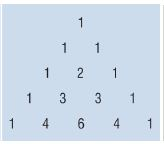
\includegraphics[width=.3\linewidth]{Pascal}
	\end{figure}
\section{Események}
	\begin{definition}
		Véletlen jelenségnek nevezzük azokat a jelenségeket, amelyeket a leírható körülmények
		nem határoznak meg egyértelműen, például: kockadobás
	\end{definition}
	\begin{definition}
		Kísérletnek nevezzük a véletlen jelenség megfigyelését.
	\end{definition}
	\begin{definition}
		Elemi esemény a kísérlet során bekövetkező lehetséges kimenetelek.
	\end{definition}
	\begin{definition}
		Eseménytér az elemi események halmaza
	\end{definition}
	\begin{definition}
		Az eseménytér részhalmazát eseménynek nevezzük.
	\end{definition}
	\begin{definition}
		Az eseménytérhez tartozó azon esemény, amely biztosan bekövetkezik, a biztos esemény,
		amely semmiképpen sem következhet be, a lehetetlen esemény. Biztos esemény jele: $H$, lehetetlen esemény jele: $\emptyset$.
	\end{definition}
\section{Műveletek eseményekkel}
	\begin{definition}
		$A$ esemény komplementere az az esemény, amely akkor következik be, amikor $A$ nem következik be. Jele: $\overline{A}$
	\end{definition}
	\begin{definition}
		$A$ és $B$ események összege az az esemény, amely akkor következik be, amikor $A$ vagy $B$ bekövetkezik. Jele: $A+B$.
	\end{definition}
	\begin{definition}
		$A$ és $B$ események szorzata az az esemény, amely akkor következik be, amikor $A$ és $B$ bekövetkezik. Jele: $A*B$.
	\end{definition}
	\begin{definition}
		$A$ és $B$ események egymást kizárják, ha egyszerre nem következhetnek be.
	\end{definition}
\section{A valószínűség-számítás alapjai}
	\begin{definition}
		Ha $n$-szer elvégzünk egy kísérletet, és $A$ esemény $k$-szor következik be, akkor az $A$ esemény relatív gyakorisága a $\frac{k}{n}$ hányados.
	\end{definition}
	\begin{definition}
		Ha sokszor elvégzünk egy kísérletet, akkor megfigyelhetjük, hogy egy $A$ esemény
		relatív gyakorisága egy szám körül ingadozik. Ezt a számot nevezzük az $A$ esemény valószínűségének. Jele: $P(A)$.
	\end{definition}
	\begin{definition}
		A valószínűség kiszámításának klasszikus modelljét akkor alkalmazhatjuk, ha egy kísérletnek véges sok kimenetele van és ezek valószínűsége egyenlő Ekkor az $A$ esemény valószínűsége:
		\begin{equation*}
			P(A)=\frac{\text{kedvező elemi események száma}}{\text{összes elemi esemény száma}}
		\end{equation*}
	\end{definition}
	\begin{outline}
		\1 Axiómák
			\2 $0\le P(A)\le1$
			\2 Biztos esemény valószínűsége 1, lehetetlen eseményé 0.
			\2 Ha $A$ és $B$ egymást kizáró események, akkor $P(A+B)=P(A)+P(B)$
			\2 $P(A+B)=P(A)+P(B)-P(A*B)$
			\2 $P(A)+P(\overline{A})=1$
	\end{outline}
	\begin{definition}
		Az $A$ esemény $B$-re vonatkozó feltételes valószínűsége: \\
		\begin{equation*}
			P(A|B)=\frac{P(A*B)}{P(B)}
		\end{equation*}
	\end{definition}
	\begin{theorem}[Bayes-tétel]
		\begin{equation*}
			P(A|B)=\frac{P(B|A)*P(A)}{P(B)}
		\end{equation*}	
	\end{theorem}
	\begin{definition}
		$A$ és $B$ események függetlenek, ha $P(A|B)=P(A)$. Ekkor $P(A*B)=P(A)*P(B)$.
	\end{definition}
	\begin{definition}
		Ha egy esemény előfordulását geometriai alakzat mértékével jellemezzük, és az esemény bekövetkezésének valószínűségét ezek hányadosával fejezzük ki, akkor geometriai valószínűségről beszélünk.
	\end{definition}
\section{Diszkrét eloszlások}
	\begin{definition}
		A valószínűségi változó az eseménytéren értelmezett valós értékű függvény. Jele: $\xi$.
	\end{definition}
	\begin{definition}
		Ha a valószínűségi változó lehetséges értékeinek száma véges vagy megszámlálhatóan végtelen, akkor diszkrét valószínűségi változóról beszélünk.
	\end{definition}
	\begin{definition}
		A visszatevés nélküli mintavétel eloszlását hipergeometrikus eloszlásnak nevezzük.
	\end{definition}
	\begin{theorem}
		Hipergeometrikus eloszlásnál van $N$ db elemünk, amelyből $M$ db elem rendelkezik egy adott $A$ tulajdonsággal, $N-M$ db pedig nem. Visszatevés nélkül kiválasztunk $n$ db-ot. Annak a valószínűsége, hogy $k$ db rendelkezik $A$ tulajdonsággal:
		\begin{equation*}
			P(\xi=k)=\frac{\binom{M}{k}*\binom{N-M}{n-k}}{\binom{N}{n}},\text{ ahol }k\le n
		\end{equation*}
	\end{theorem}
	\begin{theorem}
		Hipergeometrikus eloszlásnál $A$ tulajdonságú elemek várható értéke:
		\begin{equation*}
			M(\xi)=n*\frac{M}{N}
		\end{equation*}
	\end{theorem}
\section{Alkalmazások}
	\begin{outline}
		\1 Kiválasztási problémák: 
			\2 Hányféleképpen lehet kitölteni egy lottószelvényt?
			\2 Egy $n$ elemű halmaznak hány $k$ elemű részhalmaza van?
		\1 Klasszikus valószínűségi modell
			\2 Szerencsejátékoknál nyerési esély megállapítása
			\2 Mekkora a valószínűsége, hogy az 5-ös, 6-os lottón telitalálatos szelvényünk lesz?
	\end{outline}
\pagebreak
\section{Matematikatörténet}
	\begin{outline}
		\1 Pascal (XVII. század)
			\2 Binomiális együtthatók tanulmányozása, módszer kiszámításukra
			\2 Pascal-háromszög
		\1 Bernoulli (XVII. század)
			\2 Kombinatorikai ismeretek alkalmazása valószínűség kiszámítására
			\2 Jelentősen hozzájárult a valószínűségelmélet kifejlesztéséhez
	\end{outline}
\chapter{Valószínűségszámítás 2.}
\section{Permutációk}
	\begin{definition}
		Egy adott $n$ elemű halmaz elemeinek ismétlés nélküli permutációján az $n$ különböző elem sorba rendezését értjük.
	\end{definition}
	\begin{theorem}
		Egy $n$ elemű halmaz ismétlés nélküli permutációinak száma:
		\begin{equation*}
			\prod_{i=0}^{n-1}n-i=n!
		\end{equation*}
	\end{theorem}
	\begin{definition}
		Ha az $n$ elem között van $k_1,k_2,\dots,k_m$ egymással megegyező, akkor az elemek sorba rendezését ismétléses permutációnak nevezzük.
	\end{definition}
	\begin{theorem}
		Ha az $n$ elem között $k_1,k_2,\dots,k_m$ egymással megegyező van, és $\sum_{i=1}^{m}k_i=n$, akkor az ismétléses permutációk száma:
		\begin{equation*}
			\frac{n!}{\prod_{i=1}^{m}(k_i!)}
		\end{equation*}
	\end{theorem}
\section{Variációk}
	\begin{definition}
		Van $n$ db egymástól különböző elemünk. Ha ezekből $k\le n$ db-ot kiválasztunk úgy, hogy az elemek sorrendje számít, akkor $n$ elem $k$-ad osztályú ismétlés nélküli variációját kapjuk.
	\end{definition}
	\begin{theorem}
		$n$ elem $k$-ad osztályú ismétlés nélküli variációinak száma: $\frac{n!}{(n-k)!}$
	\end{theorem}
	\begin{definition}
		Van $n$ db egymástól különböző elemünk. Ha ezekből $k\le n$ db-ot kiválasztunk úgy, hogy az elemek sorrendje számít, és egy elemet többször is kiválaszthatunk, akkor $n$ elem $k$-ad osztályú ismétléses variációját kapjuk.
	\end{definition}
	\begin{theorem}
		$n$ elem $k$-ad osztályú ismétléses variációinak száma: $n^k$
	\end{theorem}
\section{A valószínűség-számítás alapjai}
	\begin{definition}
		Ha $n$-szer elvégzünk egy kísérletet, és $A$ esemény $k$-szor következik be, akkor az $A$ esemény relatív gyakorisága a $\frac{k}{n}$ hányados.
	\end{definition}
	\begin{definition}
		Ha sokszor elvégzünk egy kísérletet, akkor megfigyelhetjük, hogy egy $A$ esemény
		relatív gyakorisága egy szám körül ingadozik. Ezt a számot nevezzük az $A$ esemény valószínűségének. Jele: $P(A)$.
	\end{definition}
	\begin{definition}
		A valószínűség kiszámításának klasszikus modelljét akkor alkalmazhatjuk, ha egy kísérletnek véges sok kimenetele van és ezek valószínűsége egyenlő Ekkor az $A$ esemény valószínűsége:
		\begin{equation*}
		P(A)=\frac{\text{kedvező elemi események száma}}{\text{összes elemi esemény száma}}
		\end{equation*}
	\end{definition}
	\begin{outline}
		\1 Axiómák
		\2 $0\le P(A)\le1$
		\2 Biztos esemény valószínűsége 1, lehetetlen eseményé 0.
		\2 Ha $A$ és $B$ egymást kizáró események, akkor $P(A+B)=P(A)+P(B)$
		\2 $P(A+B)=P(A)+P(B)-P(A*B)$
		\2 $P(A)+P(\overline{A})=1$
	\end{outline}
	\begin{definition}
		Az $A$ esemény $B$-re vonatkozó feltételes valószínűsége: \\
		\begin{equation*}
		P(A|B)=\frac{P(A*B)}{P(B)}
		\end{equation*}
	\end{definition}
	\begin{theorem}[Bayes-tétel]
		\begin{equation*}
		P(A|B)=\frac{P(B|A)*P(A)}{P(B)}
		\end{equation*}	
	\end{theorem}
	\begin{definition}
		$A$ és $B$ események függetlenek, ha $P(A|B)=P(A)$. Ekkor $P(A*B)=P(A)*P(B)$.
	\end{definition}
	\begin{definition}
		Ha egy esemény előfordulását geometriai alakzat mértékével jellemezzük, és az esemény bekövetkezésének valószínűségét ezek hányadosával fejezzük ki, akkor geometriai valószínűségről beszélünk.
	\end{definition}
\section{Diszkrét eloszlások}
	\begin{definition}
		A valószínűségi változó az eseménytéren értelmezett valós értékű függvény. Jele: $\xi$.
	\end{definition}
	\begin{definition}
		Ha a valószínűségi változó lehetséges értékeinek száma véges vagy megszámlálhatóan végtelen, akkor diszkrét valószínűségi változóról beszélünk.
	\end{definition}
	\begin{definition}
		Binomiális eloszlás olyan kísérletnél fordul elő, amelynek 2 kimenetele lehetséges: az $A$ esemény $p$ valószínűséggel bekövetkezik, vagy $1-p$ valószínűséggel nem következik be.
	\end{definition}
	\begin{theorem}
		Binomiális eloszlásnál, ha a kísérletet $n$-szer ismételjük, akkor annak a valószínűsége, hogy az $A$ esemény $k\le n$-szer következik be:
		\begin{equation*}
			P(\xi=k)=\binom{n}{k}*p^k*(1-p)^{n-k}
		\end{equation*}
	\end{theorem}
	\begin{theorem}
		A binomiális eloszlás várható értéke: $n*p$
	\end{theorem}
	\begin{theorem}
		A binomiális eloszlás varianciája: $n*p(1-p)$
	\end{theorem}
	\begin{proof}
		$\sigma^2(\xi)=E(\xi^2)-E(\xi)^2$. Legyen $q=1-p$:
		\begin{align*}
			E(x^2)&=\sum_{k=0}^n k^2\binom{n}{k}p^kq^{n-k}=
			\sum_{k=0}^{n}k^2*\frac{n!}{k!(n-k)!}*p^kq^{n-k}=\\
			&=\sum_{k=0}^{n}k*n*\frac{(n-1)!}{(k-1)!*(n-1-(k-1))!}*p^kq^{n-k}=\sum_{k=0}^n k*n\binom{n-1}{k-1}p^kq^{n-k}=\\
			&=n*p\sum_{k=1}^nk\binom{n-1}{k-1}p^{k-1}q^{n-1-(k-1)}
		\end{align*}
		Mivel, ha $k=0$, akkor a szummán belüli kifejezés 0. Legyen $j=k-1,$ $m=n-1,$ ekkor:
		\begin{align*}
			E(x^2)&=n*p\sum_{j=0}^{m}(j+1)\binom{m}{j}p^jq^{m-j}=\\
			&=n*p\left(\sum_{j=0}^{m} \left(j\binom{m}{j}*p^jq^{m-j}\right)+ \sum_{j=0}^{m}\left(\binom{m}{j}p^jq^{m-j}\right)\right)=\\
			&=n*p\left(\sum_{j=1}^{m} \left(j\frac{m!}{j!(m-j)!}*p^jq^{m-j}\right)+ \sum_{j=0}^{m}\left(\binom{m}{j}p^jq^{m-j}\right)\right)=\\
			&=n*p\left(\sum_{j=1}^{m} \left(m\frac{(m-1)!}{(j-1)!(m-1-(j-1))!}*p^jq^{m-j}\right)+ \sum_{j=0}^{m}\left(\binom{m}{j}p^jq^{m-j}\right)\right)=\\
			&=n*p\left(\sum_{j=1}^{m} \left(m\binom{m-1}{j-1}*p^jq^{m-j}\right)+ \sum_{j=0}^{m}\left(\binom{m}{j}p^jq^{m-j}\right)\right)=\\
			&=n*p\left(m*p*\sum_{j=1}^{m}\left(\binom{m-1}{j-1}*p^{j-1}q^{m-1-(j-1)}\right)+ \sum_{j=0}^{m}\left(\binom{m}{j}p^jq^{m-j}\right)\right)
		\end{align*}
		Legyen $l=j-1,$ $k=m-1$:
		\begin{align*}
			E(x^2)&=n*p\left(m*p*\sum_{l=0}^{k}\left(\binom{k}{l}*p^{l}q^{k-l}\right)+ \sum_{j=0}^{m}\left(\binom{m}{j}p^jq^{m-j}\right)\right)=\\
			&=n*p\left(m*p*(p+q)^k+(p+q)^m\right)=n*p(m*p+1)=\\
			&=n*p((n-1)p+1)=n*p*(np-p+1)=n^2p^2-np^2+np
		\end{align*}
		Mivel tudjuk, hogy $E(x)=np\implies E^2(x)=n^2p^2$, ezért:
		\begin{align*}
			\sigma^2(x)&=E(x^2)-E^2(x)=n^2p^2-np^2+np-n^2p^2=np-np^2=np(1-p)
		\end{align*}
	\end{proof}
\section{Geometriai valószínűség}
	Adott egy pontok alkotta geometriai alakzat. Elemi eseménynek ekkor az adott ponthalmazból az
	egyik pont kiválasztása, azaz ekkor az elemi eseménynek pontokat feleltetünk meg. Egy esemény
	azt jelenti, hogy a kiválasztott pont beletartozik egy bizonyos kijelölt részponthalmazba, résztartományba, vagyis az események ponthalmazok, tartományok. Ekkor az eseménytér egy geometriai
	alakzat, az esemény ezen pontok egy bizonyos tulajdonsággal rendelkező részhalmaza, az elemi
	esemény a geometriai alakzat egy pontja.
	\begin{definition}
		Ha az esemény bekövetkezésének valószínűsége arányos a részhalmaz mértékszámával,
		akkor geometriai valószínűségéről beszélünk. Ekkor $A$ esemény valószínűsége:
		\begin{equation*}
			P(A)=\frac{\text{$A$ eseménynek megfelelő részalakzat mértéke}}{a kísérlettel kapcsolatos teljes alakzat mértéke}=\frac{m}{M}
		\end{equation*}
		A mérték lehet hosszúság, terület, térfogat.
	\end{definition}
	Példák:
	\begin{itemize}
		\item Egy adott méretű darts táblán egy bizonyos részbe való találat valószínűsége
		\item Két ember találkozásának valószínűsége egy bizonyos órában, ha egyikük sem vár 15 percnél
		többet
		\item Meteor szárazföldre való becsapódásának valószínűsége
	\end{itemize}
\section{Alkalmazások}
	\begin{outline}
		\1 Sorba rendezési problémák:
			\2 Hányféleképpen lehet kitölteni egy lottószelvényt?
		\1 Binomiális eloszlás
			\2 Mekkora a valószínűsége, hogy a totón telitalálatos szelvényünk lesz?
			\2 A gyártósorokon elkészült termékek közül a selejtek számának közelítő meghatározása várható érték segítségével.
	\end{outline}
\section{Matematikatörténet}
	\begin{outline}
		\1 Bernoulli (XVII. század)
			\2 Kombinatorikai ismeretek alkalmazása valószínűség kiszámítására
			\2 Jelentősen hozzájárult a valószínűségelmélet kifejlesztéséhez
		\1 Buffon (XVIII. század)
			\2 Tűprobléma: geometriai valószínűség fogalmának bevezetése
			\2 Egy $l$ hosszú tűt ledobunk $d$ távolságban lévő párhuzamos vonalakra
				\3 Mi a valószínűsége, hogy metszeni fog egy vonalat?
				\3 Ha $l\le d$, akkor: $\frac{2l}{\pi d}$
				\3 Ha $l>d$, akkor, hogy legalább egy vonalat metsz: $\frac{2}{\pi}*\left(x-\sqrt{x^2-1}+\arccos\frac{1}{x}\right)$, ahol $x=\frac{l}{d}>1$.
		\1 Shannon (XX. század)
			\2 Információelmélet megalapozója
				\3 Valószínűségszámítás legfiatalabb ága
	\end{outline}
\chapter{Bizonyítási módszerek}
\section{Bizonyítások a matematikában}
	A matematika különböző ágai hasonlóan épülnek fel. Meghatározunk alapfogalmakat, majd ezek	segítségével további fogalmakat definiálunk. Kimondunk axiómákat, amelyek igazságát elfogadjuk. Az axiómákból elindulva a matematikai logika eszközeivel, helyes következtetéseken keresztül további tételeket bizonyítunk be. A bizonyítás eljárási mód egy állítás helyességének indoklására a matematikai logika műveleteinek felhasználásával. A matematikai tételek általában implikációk vagy ekvivalenciák.
	
	Az implikációk bizonyítása során a feltételből helyes matematikai következtetésekkel el kell jutni
	a következményhez. Bizonyítás közben a definíciókat, axiómákat, és a már bizonyított tételeket
	felhasználhatjuk. Így belátjuk, hogy a feltétel valóban elégséges feltétele a következménynek.
	Ekvivalenciák bizonyítása során két implikációt bizonyítunk be.
\section{Direkt bizonyítás}
	\begin{definition}
		A direkt bizonyítás során igaz állításokból kiindulva matematikailag helyes következtetésekkel eljutunk a bizonyítandó állításhoz.
	\end{definition}
	\begin{theorem}
		Ha $a,b\in\mathbb{N}$, akkor
		\begin{equation*}
			7|a-2b\implies 7|10a+b
		\end{equation*}
	\end{theorem}
	\begin{proof}
		\begin{align*}
			7|a-2b&\implies a-2b=7k\ (k\in\mathbb{Z})\implies 10a-20b=70k\implies\\
			&\implies 10a-20b+b=70k+b\implies 10a+b=70k+21b
		\end{align*}
		Mivel $70k$, és $21b$ osztható 7-tel, $7|a-2b\implies 7|10a+b$
	\end{proof}
\section{Indirekt bizonyítás}
	\begin{definition}
		Az indirekt bizonyítás olyan eljárás, melynek során feltesszük, hogy a bizonyítandó állítás nem igaz, és ebből kiindulva helyes következtetésekkel lehetetlen következményekhez jutunk el. Így a kiinduló feltevés volt téves, vagyis a bizonyítandó állítás valójában igaz.
	\end{definition}
	\begin{theorem}
		$\sqrt{2}$ irracionális szám.
	\end{theorem}
	\begin{proof}
		A bizonyítás indirekt módon történik. Tegyük fel, hogy 
		\begin{equation}\label{eq:24.1}
		\sqrt{2}=\frac{a}{b}\qquad a\wedge b\in\mathbb{Z}\wedge b\ne0\wedge(a;b)=1
		\end{equation}
		Ebből következik, hogy:
		\begin{equation}
		2=\frac{a^2}{b^2}\implies a^2=2b^2
		\end{equation}
		Az egyenlet jobb oldalán szereplő szám prímtényezős felbontásában a 2 páros kitevőn szerepel, míg a bal oldalon levő szám prímtényezős felbontásában a 2 kitevője páratlan.
		
		Ez azonban lehetetlen, hiszen a számelmélet alaptétele szerint egy pozitív egész számnak
		nincs két lényegesen különböző felbontása. 
		
		Emiatt \eqref{eq:24.1} hamis, vagyis $\sqrt{2}$ irracionális.
	\end{proof}
\section{Teljes indukció}
	\begin{definition}
		A teljes indukció olyan állítások bizonyítására alkalmas, melyek $n$ pozitív egész számtól függenek. Jelöljük az állítást $P$-vel, illetve jelölje $P(n)$, hogy $P$ igaz $n$-re. A teljes indukciós eljárás során először bebizonyítjuk az állítást a kezdeti értékre, majd bizonyítjuk, hogy $P(k)\implies P(k+1)$. Ezzel az állítást minden $n$ pozitív egész számra belátjuk.
	\end{definition}
	\begin{theorem}
		Az első $n$ pozitív egész szám négyzetének összege: $\frac{n(n+1)(2n+1)}{6}$.
	\end{theorem}
	\begin{proof}
		A bizonyítás teljes indukcióval történik. Ha $n=1$, akkor $1^2=1=\frac{1*2*3}{6}=1$. Tegyük fel, hogy $n=k$-ra igaz az állítás, azaz: $\sum_{i=1}^{k} i^2=\frac{k(k+1)(2k+1)}{6}$. Be kéne látni, hogy $\sum_{i=1}^{k+1} i^2=\frac{(k+1)(k+2)(2k+3)}{6}$.
		\begin{align*}
			\sum_{i=1}^{k+1} i^2&=\frac{k(k+1)(2k+1)}{6}+(k+1)^2=(k+1)*\frac{k(2k+1)+6(k+1)}{6}=\\
			&=(k+1)*\frac{2k^2+k+6k+6}{6}=\frac{(k+1)(k+2)(2k+3)}{6}
		\end{align*}
		Vagyis az állítás teljesül $\forall n\in\mathbb{N}^+$.
	\end{proof}
\section{Skatulya-elv}
	\begin{theorem}
		Ha $n$ db skatulyába $k*n$ db-nál több elemet kell szétosztani, akkor a skatulyák valamelyikébe legalább $k+1$ elem kerül $(n,k\in\mathbb{Z})$.
	\end{theorem}
	\begin{theorem}
		$n+1$ db pozitív egész szám között biztosan van 2 olyan, amelyek különbsége osztható n-el.
	\end{theorem}
	\begin{proof}
		Legyen $n$ db skatulya az $n$-el való osztási maradékok. Mivel $n+1$ db szám van, biztosan lesz olyan skatulya, ahova 2 szám kerül. Ennek a 2 számnak a különbsége osztható $n$-el.
	\end{proof}
\section{Alkalmazások}
	\begin{outline}
		\1 Teljes indukció:
			\2 Rekurzívan definiált sorozatoknál n-edik tag általános képletének bizonyítása
		\1 Direkt bizonyítás:
			\2 Implikációk bizonyítása
	\end{outline}
\section{Matematikatörténet}
	\begin{outline}
		\1 Maurolicio (XVI. század)	
			\2 Első teljes indukció: első $n$ páratlan szám összege
		\1 Dirichlet (XIX. század)
			\2 Skatulyaelv bizonyítása
		\1 Vi\`ete ugrás (1988. IMO 6. feladat)
			\2  Indirekt bizonyítás
			\2 Legyen $a,b\in\mathbb{N}^+$, $(ab+1)|\left(a^2+b^2\right)$. Bizonyítsuk, hogy $\frac{a^2+b^2}{ab+1}$ teljes négyzet.
			\2 Indirekt bizonyítás
			\2 Legyen $k\in\mathbb{Z}^+$ úgy, hogy nem teljes négyzet. Tegyük fel, hogy: $\exists (a,\ b)\ k=\frac{a^2+b^2}{ab+1}$.
			\2 Legyenek $(A,\ B)\in\mathbb{Z}^+$, amikre: $k=\frac{A^2+B^2}{AB+1}$ úgy, hogy $A+B$ minimális. Az általánosság megszorítása nélkül feltehetjük, hogy $A\ge B$.
			\2 $A$ helyére $x$-et írva:
				\begin{align*}
					k&=\frac{x^2+B^2}{xB+1}\\
					kxB+k&=x^2+B^2\\
					x^2-(kB)x+(B^2-k)&=0
				\end{align*}
			\2 Tudjuk, hogy az egyik gyök: $x_1=A$. A másik gyökre igaz, hogy:
				\begin{equation*}
					x_2=kB-A\wedge x_2=\frac{B^2-k}{A}
				\end{equation*}
			\2 Első kifejezés miatt: $x_2\in\mathbb{Z}$. A másodikból: $x_2\ne0$, mert $k$ nem teljes négyzet
			\2 $\frac{x_2^2+B^2}{x_2B+1}=k>0\implies x_2>0$, mert a számláló, és a tört értéke pozitív, így a nevezőnek is pozitívnak kell lennie: $x_2B+1>0\implies x_2B>-1$. Mivel $B$ pozitív egész, $x_2$ nem lehet negatív.
			\2[] \begin{align*}
				A&\ge B\tag{Mivel mindkét oldal pozitív}\\
				A^2&\ge B^2\\
				A^2-k&\ge B^2-k\tag{Mivel $A>0$}\\
				A-\frac{k}{A}&\ge \frac{B^2-k}{A}\\
				\frac{B^2-k}{A}&\le A-\frac{k}{A}<A\\
				x_2&<A\\
				x_2+B&<A+B
			\end{align*}
			\2 Ez azonban ellentmond $(A,\ B)$ minimalitásának
	\end{outline}
\end{document}